% !TeX root = thesis.tex
% !BIB program = biber
% !TEX program = xelatex

%!TEX root = ../thesis.tex

% This information is used in titlepage, colophon, preface and hyperref setup (pdf metainfo), and other options.

%\def\thesistypeabbr{B.Eng.}
%\def\thesistype    {Bachelor of Engineering}
%\def\thesistypeabbr{B.Sc.Eng.}
%\def\thesistype    {Bachelor of Science in Engineering}
%\def\thesistypeabbr{M.Sc.}
%\def\thesistype    {Master of Science in Engineering}
\def\thesistypeabbr{Ph.D.}
\def\thesistype    {Doctor of Philosophy}

\def\thesisdepshort{DTU Compute}
\def\thesisdep     {Department of Applied Mathematics and Computer Science}

\def\thesisauthor  {Jakob Drachmann Havtorn}
\def\thesistitle   {Uncertainty Estimation for Machine Learning Systems}
\def\thesissubtitle{Self-assessment on Medical Conversations}
\def\thesislocation{Copenhagen}
\def\thesisyear    {2023}
\def\thesismonth   {August}
\def\thesisday     {31}

\def\papersize     {b5paper} % Final papersize (b5paper/a4paper), recommended papersize for DTU Compute is b5paper
\def\showtrims     {false}   % Print on larger paper than \papersize and show trim marks (true/false)?
\def\showframe     {false}   % Show frame of writeable area, marginparsep and marginpar (true/false)?

\def\showtodos     {true}    % Show todos (true/false)?
\def\confidential  {false}   % Confidential thesis (true/false)?


%!TEX root = ../thesis.tex

% Package that captures and warns against deprecated LaTeX patterns and syntax.
% Included first to capture from document top.
\RequirePackage[l2tabu,orthodox]{nag}

% Paper size switch command (used in \documentclass which is in main file, in order to identify it as such)
\newcommand{\papersizeswitch}[3]{\ifnum\strcmp{\papersize}{#1}=0#2\else#3\fi}
\papersizeswitch{a4paper}{\def\classfontsize{10pt}}{\def\classfontsize{10pt}}


\documentclass[\classfontsize,\papersize,twoside,showtrims,extrafontsizes]{memoir}  % identifies main document in Overleaf

%!TEX root = ../thesis.tex

\RequireXeTeX

\showtrimsoff
\papersizeswitch{b5paper}{
    % Stock and paper layout
    \pagebv
    \setlrmarginsandblock{24mm}{20mm}{*}
    \setulmarginsandblock{30mm}{30mm}{*}
    \setheadfoot{8mm}{10mm}
    \setlength{\headsep}{7mm}
    \setlength{\marginparwidth}{18mm}
    \setlength{\marginparsep}{2mm}
}{
    \papersizeswitch{a4paper}{
        \pageaiv
        \setlength{\trimtop}{0pt}
        \setlength{\trimedge}{\stockwidth}
        \addtolength{\trimedge}{-\paperwidth}
        \settypeblocksize{634pt}{448.13pt}{*}
        \setulmargins{2cm}{*}{*}
        \setlrmargins{*}{*}{*}
        \setmarginnotes{17pt}{51pt}{\onelineskip}
        \setheadfoot{\onelineskip}{2\onelineskip}
        \setheaderspaces{*}{2\onelineskip}{*}
    }{
    }
}
\ifnum\strcmp{\showtrims}{true}=0
    % For printing B5 on A4 with trimmarks
    \showtrimson
    \papersizeswitch{b5paper}{\stockaiv}{\stockaiii}
    \setlength{\trimtop}{\stockheight}
    \addtolength{\trimtop}{-\paperheight}
    \setlength{\trimtop}{0.5\trimtop}
    \setlength{\trimedge}{\stockwidth}
    \addtolength{\trimedge}{-\paperwidth}
    \setlength{\trimedge}{0.5\trimedge}
    
    % bigger todos if trim marks
    \setmarginnotes{10pt}{95pt}{\onelineskip}

    \trimLmarks
    
    % put jobname in left top trim mark
    \renewcommand*{\tmarktl}{%
      \begin{picture}(0,0)
        \unitlength 1mm
        \thinlines
        \put(-2,0){\line(-1,0){18}}
        \put(0,2){\line(0,1){18}}
        \put(3,15){\normalfont\ttfamily\fontsize{8bp}{10bp}\selectfont\jobname\ \
          \today\ \ 
          \printtime\ \ 
          Page \thepage}
      \end{picture}}

    % Remove middle trim marks for cleaner layout
    \renewcommand*{\tmarktm}{}
    \renewcommand*{\tmarkml}{}
    \renewcommand*{\tmarkmr}{}
    \renewcommand*{\tmarkbm}{}
\fi

\checkandfixthelayout                 % Check if errors in paper format!
\sideparmargin{outer}                 % Put sidemargins in outer position

% Large environments
\usepackage{microtype}
\usepackage{mathtools}
\usepackage{listings}                 % Source code printer for LaTeX
\usepackage{tikz}
\usepackage{ragged2e}

% Links
\usepackage[hyphens]{url}             % Allow hyphens in URL's
\usepackage[unicode=false,psdextra]{hyperref}                 % References package

% Graphics and colors
\usepackage{graphicx}                 % Including graphics and using colours
\usepackage{xcolor}                   % Defined more color names
\usepackage{eso-pic}                  % Watermark and other bag
\usepackage{preamble/dtucolors}
\graphicspath{{graphics/}}
\usepackage{caption}
\usepackage[labelformat=simple]{subcaption}
\usepackage[figuresleft]{rotating}


% Language
% \usepackage{polyglossia}    % multilingual typesetting and appropriate hyphenation
% \setdefaultlanguage{english}
\usepackage[english]{babel}
\usepackage{csquotes}       % language sensitive quotation facilities

% Bibliography (references)
% https://tex.stackexchange.com/questions/89842/how-to-print-only-year-no-day-month-with-biblatex            
\usepackage[backend=biber,
            natbib=true, 
            style=numeric,
            abbreviate=false,
            dateabbrev=false,
            maxbibnames=14,
            urldate=short,
            backref=true,
            alldates=year]{biblatex}
\renewcommand*{\bibfont}{\normalfont\footnotesize}  % make bibliography font smaller


\DefineBibliographyStrings{english}{%
  backrefpage = {cited on page},  % originally "cited on page"
  backrefpages = {cited on pages},  % originally "cited on pages"
}

% \newcommand{\printpublication}[1]{\AtNextCite{\defcounter{maxnames}{99}}\fullcite{#1}}  % create new command \printpublication that lists all authors
\preto\fullcite{\AtNextCite{\defcounter{maxnames}{99}}}  % make \fullcite list all authors

\DefineBibliographyExtras{english}{%
  \protected\def\mkbibdatelong#1#2#3{%
    \iffieldundef{#3}
      {}
      {\thefield{#3}%
       \iffieldundef{#2}{}{\nobreakspace}}%
    \iffieldundef{#2}
      {}
      {\mkbibmonth{\thefield{#2}}%
       \iffieldundef{#1}{}{\space}}%
    \iffieldbibstring{#1}{\bibstring{\thefield{#1}}}{\stripzeros{\thefield{#1}}}}%
}


% Highlight own author name
\usepackage{xstring}
\usepackage{etoolbox}
\newboolean{bold}
\newcommand{\makeauthorsbold}[1]{%
  \DeclareNameFormat{author}{%
  \setboolean{bold}{false}%
    \renewcommand{\do}[1]{\expandafter\ifstrequal\expandafter{\namepartfamily}{####1}{\setboolean{bold}{true}}{}}%
    \docsvlist{#1}%
    \ifthenelse{\value{listcount}=1}
    {%
      {\expandafter\ifthenelse{\boolean{bold}}{\mkbibbold{\namepartfamily\addcomma\addspace \namepartgiveni}}{\namepartfamily\addcomma\addspace \namepartgiveni}}%
    }{\ifnumless{\value{listcount}}{\value{liststop}}
      {\expandafter\ifthenelse{\boolean{bold}}{\mkbibbold{\addcomma\addspace \namepartfamily\addcomma\addspace \namepartgiveni}}{\addcomma\addspace \namepartfamily\addcomma\addspace \namepartgiveni}}%
      {\expandafter\ifthenelse{\boolean{bold}}{\mkbibbold{\addcomma\addspace \namepartfamily\addcomma\addspace \namepartgiveni\addcomma\isdot}}{\addcomma\addspace \namepartfamily\addcomma\addspace \namepartgiveni\addcomma\isdot}}%
      }
    \ifthenelse{\value{listcount}<\value{liststop}}
    {\addcomma\space}{}
  }
}
\makeauthorsbold{Havtorn}


% Floating objets, captions and references
% \usepackage{flafter}  % floats is positioned after or where it is defined! 
\setfloatlocations{figure}{tbhp}   % Set floats for all figures
\setfloatlocations{table}{tbhp}    % Set floats for all tables
\setFloatBlockFor{section}         % Typeset floats before each section
\usepackage[noabbrev,nameinlink,capitalise]{cleveref}  % Clever references. Options: "fig. !1!" --> "!Figure 1!"
\hangcaption
\captionnamefont{\bfseries}
\subcaptionlabelfont{\bfseries}
\newsubfloat{figure}
\newsubfloat{table}
%\letcountercounter{figure}{table}         % Consecutive table and figure numbering
%\letcountercounter{lstlisting}{table}     % Consecutive table and listings numbering
\captiontitlefinal{.}
% strip things from equation references, making them "(1)" instead of "Equation~1"
% from http://tex.stackexchange.com/questions/122174/how-to-strip-eq-from-cleveref
\crefformat{equation}{(#2#1#3)}
\crefrangeformat{equation}{(#3#1#4) to~(#5#2#6)}
\crefmultiformat{equation}{(#2#1#3)}%
{ and~(#2#1#3)}{, (#2#1#3)}{ and~(#2#1#3)}


% Lowercase and uppercase versions of \nameref 
% (from https://tex.stackexchange.com/questions/445404/capitalization-variants-of-nameref)
% - fucnameref: First letter in first word is uppercased
% - ucnameref: All words are uppercased
% - lcnameref: All words are lowercased
\makeatletter
\AtBeginDocument{%
  \newcommand\My@Macro[1]{#1}%
  \newcommand\My@Thirdoffive[5]{\My@Macro{#3}}%
  \renewcommand*\@namerefstar[1]{%
    \HyRef@StarSetRef{#1}\My@Thirdoffive
  }%
  \renewcommand*\T@nameref[1]{%
    \begingroup
    \let\label\@gobble
    \NR@setref{#1}\My@Thirdoffive{#1}%
    \endgroup
  }%
  \DeclareRobustCommand\fucnameref{%
    \@ifstar\fucnameref@star\fucnameref@nostar
  }%
  \newcommand\callemakefirstuc[1]{%
    \MakeLowercase{\emakefirstuc{#1}}%
  }%
  \newcommand\fucnameref@star[1]{%
    \begingroup
    \let\My@Macro=\callemakefirstuc
    \nameref*{#1}%
    \endgroup
  }%
  \newcommand\fucnameref@nostar[1]{%
    \begingroup
    \let\My@Macro=\callemakefirstuc
    \nameref{#1}%
    \endgroup
  }%
  \DeclareRobustCommand\ucnameref{%
    \@ifstar\ucnameref@star\ucnameref@nostar
  }%
  \newcommand\ucnameref@star[1]{%
    \begingroup
    \MFUhyphentrue
    \let\My@Macro=\ecapitalisefmtwords
    \nameref*{#1}%
    \endgroup
  }%
  \newcommand\ucnameref@nostar[1]{%
    \begingroup
    \MFUhyphentrue
    \let\My@Macro=\ecapitalisefmtwords
    \nameref{#1}%
    \endgroup
  }%
  \DeclareRobustCommand\lcnameref{%
    \@ifstar\lcnameref@star\lcnameref@nostar
  }%
  \newcommand\lcnameref@star[1]{%
    \begingroup
    \let\My@Macro=\MakeLowercase
    \nameref*{#1}%
    \endgroup
  }%
  \newcommand\lcnameref@nostar[1]{%
    \begingroup
    \let\My@Macro=\MakeLowercase
    \nameref{#1}%
    \endgroup
  }%
}%
\makeatother


% Table of contents (TOC)
\setcounter{tocdepth}{1}                    % Depth of table of content
\setcounter{secnumdepth}{2}                 % Depth of section numbering
\setcounter{maxsecnumdepth}{3}              % Max depth of section numbering
\renewcommand{\cftdot}{}                    % Remove dots in ToC

\RequirePackage{tocloft}
\PassOptionsToPackage{titles}{tocloft}

% \MakeUppercase breaks hyperlinks
% https://tex.stackexchange.com/questions/605022/how-can-i-use-makeuppercase-in-patchcmd-without-breaking-hyperlinks
% https://groups.google.com/g/comp.text.tex/c/eiLmTiZjKcM
\def\tocnumbersize{\footnotesize}

\renewcommand{\cftpartpresnum}{\scshape}
\renewcommand{\cftpartfont}{\normalsize\color{dtured}\scshape\MakeLowercase}              % \part font in ToC
\renewcommand{\cftpartpagefont}{\tocnumbersize}                                           % \part font in ToC

\renewcommand{\cftchapterpresnum}{\tocnumbersize}%
\renewcommand{\cftchapterfont}{\normalsize\scshape}                                       % \chapter font in ToC
\renewcommand{\cftchapterpagefont}{\tocnumbersize}                                        % \chapter font in ToC

\renewcommand{\cftsectionpresnum}{\tocnumbersize}%
\renewcommand{\cftsectionfont}{\small}                                                    % \section font in ToC
\renewcommand{\cftsectionpagefont}{\tocnumbersize}                                        % \section font in ToC

\renewcommand{\cftsubsectionpresnum}{\tocnumbersize}%
\renewcommand{\cftsubsectionfont}{\small}                                                 % \subsection font in ToC
\renewcommand{\cftsubsectionpagefont}{\tocnumbersize}                                     % \subsection font in ToC

\renewcommand{\cftsubsubsectionpresnum}{\tocnumbersize}%
\renewcommand{\cftsubsubsectionfont}{\small}                                              % \subsubsection font in ToC
\renewcommand{\cftsubsubsectionpagefont}{\tocnumbersize}                                  % \subsubsection font in ToC

\setlength{\cftbeforepartskip}{1em}%
\setlength{\cftbeforechapterskip}{.3em}%
% \setlength{\cftbib}{\cftbeforepartskip}%


% \renewcommand*{\parttitlefont}{\normalfont\large\MakeUppercase}  % font for part title
% \renewcommand*{\partnamefont}{\normalfont\scshape} % font for part name
% \renewcommand*{\partnumfont}{\normalfont\scshape\MakeLowercase}  % font for part number



% Todos
\usepackage{totcount}                                                               % For total counting of counters
\def\todoshowing{}
\ifnum\strcmp{\showtodos}{false}=0
    \def\todoshowing{disable}
\fi
\usepackage[colorinlistoftodos,\todoshowing]{todonotes}                             % Todonotes package for nice todos
\newtotcounter{todocounter}                                                         % Creates counter in todo
\let\oldtodo\todo
\newcommand*{\newtodo}[2][]{\stepcounter{todocounter}\oldtodo[#1]{\thesection~(\thetodocounter)~#2}}
\let\todo\newtodo
\let\oldmissingfigure\missingfigure
\newcommand*{\newmissingfigure}[2][]{\stepcounter{todocounter}\oldmissingfigure[#1]{\thesection~(\thetodocounter)~#2}}
\let\missingfigure\newmissingfigure
\makeatletter
\newcommand*{\mylistoftodos}{% Only show list if there are todos
\if@todonotes@disabled
\else
    \ifnum\totvalue{todocounter}>0
        \markboth{\@todonotes@todolistname}{\@todonotes@todolistname}
        \phantomsection\todototoc
        \listoftodos
    \else
    \fi
\fi
}
\makeatother
\newcommand{\lesstodo}[2][]{\todo[color=green!40,#1]{#2}}
\newcommand{\moretodo}[2][]{\todo[color=red!40,#1]{#2}}


% Chapterstyle
\makeatletter
\makechapterstyle{mychapterstyle}{
    % \chapnamefont
    % \chaptitlefont
    % \printchaptername
    % \printchapternum
    % \printchapternonum
    % \chapternamenum

    \chapterstyle{default}

    \setlength\beforechapskip{0mm}

    \def\format{\normalfont}  % \def\format{\normalfont\sffamily}
    \renewcommand*{\chapnamefont}{\format\fontshape{sc}\selectfont}  % font for chapter text
    % \renewcommand*{\chapnumfont}{\format\fontsize{30}{30}\fontshape{sc}\selectfont}  % font for chapter number
    \renewcommand*{\chapnumfont}{\format\fontsize{18}{18}\fontfamily{eulervm}\selectfont}  % font for chapter number
    \renewcommand*{\chaptitlefont}{\format\fontsize{16}{16}\fontshape{sc}\selectfont}  % font for chapter title

    \renewcommand*{\printchaptername}{\chapnamefont\MakeUppercase{\@chapapp}}  % Uppercase all characters in name
    \patchcommand{\printchaptername}{\begingroup\color{dtured}}{\endgroup}
    \renewcommand*{\chapternamenum}{\space}
    \patchcommand{\printchapternum}{\begingroup\color{dtured}}{\endgroup}
    % \renewcommand*{\printchapternonum}{%
    %     \vphantom{\printchaptername\chapternamenum\chapnumfont 1}
    %     \afterchapternum
    % }

    \setlength\midchapskip{1ex}

    % \renewcommand*{\printchaptertitle}[1]{\raggedleft \chaptitlefont ##1}
    \renewcommand*{\printchaptertitle}[1]{\raggedright \chaptitlefont ##1}
    \renewcommand*{\afterchaptertitle}{\vskip0.5\onelineskip \hrule \vskip1.3\onelineskip}
}
\makeatother
\chapterstyle{mychapterstyle}


% Part style
% \renewcommand*{\thepart}{\arabic{part}}  % redefine the format of the part counter
\renewcommand*{\parttitlefont}{\normalfont\LARGE\scshape}  % font for part title
\renewcommand*{\partnamefont}{\normalfont\large\scshape} % font for part name
\renewcommand*{\partnumfont}{\normalfont\large\scshape}  % font for part number
% Part name and number
\renewcommand*{\printpartname}{{\color{dtured}\partnamefont PART}}  % Command for printing the part name
\renewcommand*{\printpartnum}{{\color{dtured}\partnumfont\thepart}} % Command for printing the part number
% Define skips (used to add horizontal rule)
\renewcommand{\midpartskip}{\par\parbox{0.25\textwidth}{\hrulefill}\par}
\renewcommand{\beforepartskip}{\vspace*{\fill}}
\renewcommand{\afterpartskip}{\vspace*{\fill}}
% For table of contents
\renewcommand*{\cftpartname}{Part}
\renewcommand*{\cftpartpresnum}{\space}
\renewcommand*{\cftpartaftersnum}{.}
\renewcommand*{\cftpartaftersnumb}{\space}


% Header and footer
\def\hffont{\scshape\small}
\makepagestyle{myruled}
\makeheadrule{myruled}{\textwidth}{\normalrulethickness}
\makeevenhead{myruled}{\hffont\thepage}{}{\hffont\leftmark}
\makeoddhead{myruled}{\hffont\rightmark}{}{\hffont\thepage}
\makeevenfoot{myruled}{}{}{}
\makeoddfoot{myruled}{}{}{}
\makepsmarks{myruled}{
    \nouppercaseheads
    \createmark{chapter}{both}{shownumber}{}{\space}
    \createmark{section}{right}{shownumber}{}{\space}
    \createplainmark{toc}{both}{\contentsname}
    \createplainmark{lof}{both}{\listfigurename}
    \createplainmark{lot}{both}{\listtablename}
    \createplainmark{bib}{both}{\bibname}
    \createplainmark{index}{both}{\indexname}
    \createplainmark{glossary}{both}{\glossaryname}
}
\pagestyle{myruled}
\copypagestyle{cleared}{myruled}      % When \cleardoublepage, use myruled instead of empty
\makeevenhead{cleared}{\hffont\thepage}{}{} % Remove leftmark on cleared pages

\makeevenfoot{plain}{}{}{}            % No page number on plain even pages (chapter begin)
\makeoddfoot{plain}{}{}{}             % No page number on plain odd pages (chapter begin)

% \*section, \*paragraph font styles
\setsecheadstyle              {\Large\scshape\raggedright} %{\LARGE\sffamily\raggedright}
\setsubsecheadstyle           {\large\scshape\raggedright} %{\Large\sffamily\raggedright}
\setsubsubsecheadstyle        {\normalsize\scshape\raggedright} %{\large\sffamily\raggedright}
% \setparaheadstyle             {\normalsize\sffamily\itseries\raggedright}
% \setsubparaheadstyle          {\normalsize\sffamily\raggedright}


% Hypersetup
\hypersetup{
    pdfauthor={\thesisauthor{}},
    pdftitle={\thesistitle{}},
    pdfsubject={\thesissubtitle{}},
    pdfdisplaydoctitle,
    bookmarksnumbered=true,
    bookmarksopen,
    breaklinks,
    linktoc=all,
    plainpages=false,
    unicode=true,
    colorlinks=false,
    citebordercolor=dtured,           % color of links to bibliography
    filebordercolor=dtured,           % color of file links
    linkbordercolor=dtured,           % color of internal links (change box color with linkbordercolor)
    urlbordercolor=s13,               % color of external links
    hidelinks,                        % Do not show boxes or colored links.
}
% Hack to make right pdfbookmark link. The normal behavior links just below the chapter title. This hack put the link just above the chapter like any other normal use of \chapter.
% Another solution can be found in http://tex.stackexchange.com/questions/59359/certain-hyperlinks-memoirhyperref-placed-too-low
\makeatletter
\renewcommand{\@memb@bchap}{%
  \ifnobibintoc\else
    \phantomsection
    \addcontentsline{toc}{chapter}{\bibname}%
  \fi
  \chapter*{\bibname}%
  \bibmark
  \prebibhook
}
\let\oldtableofcontents\tableofcontents
\newcommand{\newtableofcontents}{
    \@ifstar{\oldtableofcontents*}{
        \phantomsection\addcontentsline{toc}{chapter}{\contentsname}\oldtableofcontents*}}
\let\tableofcontents\newtableofcontents
\makeatother

% Confidential
\newcommand{\confidentialbox}[1]{
    \put(0,0){\parbox[b][\paperheight]{\paperwidth}{
        \begin{vplace}
            \centering
            \scalebox{1.3}{
                \begin{tikzpicture}
                    \node[very thick,draw=red!#1,color=red!#1,
                          rounded corners=2pt,inner sep=8pt,rotate=-20]
                          {\sffamily \HUGE \MakeUppercase{Confidential}};
                \end{tikzpicture}
            }
        \end{vplace}
    }}
}

% Prefrontmatter
\newcommand{\prefrontmatter}{
    \pagenumbering{alph}
    \ifnum\strcmp{\confidential}{true}=0
        \AddToShipoutPictureBG{\confidentialbox{10}}   % 10% classified box in background on each page
        \AddToShipoutPictureFG*{\confidentialbox{100}} % 100% classified box in foreground on first page
    \fi
}

% DTU frieze
\newcommand{\frieze}[2]{%
    \AddToShipoutPicture*{
        \put(#1,#2){
            \parbox[b][\paperheight]{\paperwidth}{%
                \includegraphics[trim=130mm 0 0 0,width=0.9\textwidth]{DTU-frise-SH-15}
                \vspace*{2.5cm}
            }
        }
    }
}

% This is a double sided book. If there is a last empty page lets use it for some fun e.g. the frieze.
% NB: For a fully functional hack the \clearpage used in \include does some odd things with the sequence numbering. Thefore use \input instead of \include at the end of the book. If bibliography is used at last everything should be ok.
\makeatletter
% Adjust so gatherings is allowd for single sheets too! (hacking functions in memoir.dtx)
\patchcmd{\leavespergathering}{\ifnum\@memcnta<\tw@}{\ifnum\@memcnta<\@ne}{
    \leavespergathering{1}
    % Insert the frieze
    \patchcmd{\@memensuresigpages}{\repeat}{\repeat\frieze{0}{0}}{}{}
}{}
\makeatother


% %% Sharelatex fix for microtype warnings
% \makeatletter
% \def\MT@is@composite#1#2\relax{%
%   \ifx\\#2\\\else
%     \expandafter\def\expandafter\MT@char\expandafter{\csname\expandafter
%                     \string\csname\MT@encoding\endcsname
%                     \MT@detokenize@n{#1}-\MT@detokenize@n{#2}\endcsname}%
%     % 3 lines added:
%     \ifx\UnicodeEncodingName\@undefined\else
%       \expandafter\expandafter\expandafter\MT@is@uni@comp\MT@char\iffontchar\else\fi\relax
%     \fi
%     \expandafter\expandafter\expandafter\MT@is@letter\MT@char\relax\relax
%     \ifnum\MT@char@ < \z@
%       \ifMT@xunicode
%         \edef\MT@char{\MT@exp@two@c\MT@strip@prefix\meaning\MT@char>\relax}%
%           \expandafter\MT@exp@two@c\expandafter\MT@is@charx\expandafter
%             \MT@char\MT@charxstring\relax\relax\relax\relax\relax
%       \fi
%     \fi
%   \fi
% }
% % new:
% \def\MT@is@uni@comp#1\iffontchar#2\else#3\fi\relax{%
%   \ifx\\#2\\\else\edef\MT@char{\iffontchar#2\fi}\fi
% }
% \makeatother\makeatother

%!TEX root = ../thesis.tex

% Math symbols
% \usepackage{amsmath}
% \usepackage{amssymb}

% Text fonts (http://www.macfreek.nl/memory/Fonts_in_LaTeX)
% Install fonts from /usr/local/texlive/<version>/texmf-dist/fonts/opentype/public
% \usepackage[utf8]{inputenc}
\usepackage{fontspec}
% \usepackage[T1]{fontenc}
% \usepackage{lmodern}
\usepackage{slantsc}
% \RequirePackage{fix-cm}
\usepackage{bold-extra}
\usepackage{csquotes}       % language sensitive quotation facilities


% Method that works with TeXLive 2023
% \usepackage[math-style=upright]{unicode-math}
% \setmainfont{texgyrepagella-regular.otf}[Scale=1.0, Ligatures={Common,Rare,TeX}]  % Or Palatino Linotype, etc.
% \setmathfont{texgyrepagella-math.otf}[Scale=MatchLowercase]
% \setmathfont{euler.otf}[range={up/{Latin,latin,Greek,Greek}, bfup/{Latin,latin,Greek,Greek}, cal, bfcal, frak, bffrak}, Scale=MatchLowercase, script-features={}, sscript-features={}]


% Method that works with TeXLive 2023 and is simpler and has fewer missing characters
\usepackage{newpxtext, eulerpx}


% Method that should be best practice for TeXLive
% These packages were recommended but seem to cause trouble with the euler-math and unicode-math packages.
% \usepackage{newpxtext,newpxmath}
% \setmainfont{texgyrepagella-regular.otf}[Scale=1.0, Ligatures={Common,Rare,TeX}]  % Or Palatino Linotype, etc.
% \usepackage{euler-math}


% Method that works with TeXLive 2022 (but is missing some special characters e.g. ê, ç)
% \usepackage{amssymb}
% \usepackage{upgreek}
% \usepackage{mathpazo}
% \usepackage[OT1,euler-digits]{eulervm}
% \renewcommand{\mathbf}{\mathbold}  % euler requires \mathbold for bold math





% % Remove: "Font shape `T1/eulervm/m/n' undefined (Font) using `T1/cmr/m/n' instead."
% \usepackage{substitutefont}
% \substitutefont{TS1}{eulervm}{cmr}

%
% [
%   Extension=.otf,
%   UprightFont=*-regular,
%   ItalicFont=*-italic,
%   BoldFont=*-bold,
%   BoldItalicFont=*-bolditalic,
%   BoldSmallCapsFont=*-boldsmallcaps,
%   Numbers=OldStyle,
% ]

% \setmainfont{QTPalatine}

% \DeclareCharacterInheritance
%    { encoding = {TU,EU1,EU2},
%      family   = {QTPalatine} }
%    { A = {\`A,\'A,\^A,\~A,\"A,\r A},
%      a = {\`a,\'a,\^a,\~a,\"a,\r a},
%      C = {\c C},
%      c = {\c c},
%      D = {\DH},
%      d = {\dj},
%      E = {\`E,\'E,\^E,\"E},
%      e = {\`e,\'e,\^e,\"e},
%      I = {\`I,\'I,\^I,\"I},
%      i = {\`i,\'i,\^i,\"i,\i},
%      L = {\L},
%      l = {\l},
%      N = {\~N},
%      n = {\~n},
%      O = {\O,\`O,\'O,\^O,\~O,\"O},
%      o = {\o,\`o,\'o,\^o,\~o,\"o},
%      S = {\v S},
%      s = {\v s},
%      U = {\`U,\'U,\^U,\"U},
%      u = {\`u,\'u,\^u,\"u},
%      Y = {\'Y,\"Y},
%      y = {\'y,\"y},
%      Z = {\v Z},
%      z = {\v z}
%    }


% % Sans-serif font
% \setsansfont[
%     Ligatures=TeX,
%     Extension=.otf,
%     UprightFont=*-regular,
%     BoldFont=*-bold,
%     ItalicFont=*-italic,
%     BoldItalicFont=*-bolditalic,
%     % SlantedFont=,
%     % BoldSlantedFont=,
%     % SmallCapsFont=
%     Scale=0.8      % Adjustmens when using math in sections
% ]{texgyreadventor}


% Monospaced
% \setmonofont[Scale=MatchLowercase]{Linux Biolinum O}

%\setsansfont[Ligatures=TeX]{Neo Sans Intel}    % Neo Sans Intel – Like DTU font but more symbols
%\setsansfont[
%    Ligatures=TeX,
%    Scale=0.8
%]{NeoSans}           % NeoSans – DTU font (missing `+' symbols and other)
% \setsansfont[Ligatures=TeX]{CMU Sans Serif}    % Computer Modern Unicode font
%\setsansfont[Ligatures=TeX]{Latin Modern Sans} % Latin Modern Sans serif font

% Use this for more convienent sans serif font in math mode.
%\setmathsf{Latin Modern Sans}

\input{preamble/etc}
%!TEX root = ../Thesis.tex

% Parenthesis
\providecommand{\pa}[1]{{\left(#1\right)}}
  \renewcommand{\pa}[1]{{\left(#1\right)}}
\providecommand{\bra}[1]{{\left[#1\right]}}
  \renewcommand{\bra}[1]{{\left[#1\right]}}
\providecommand{\cbra}[1]{{\left\{#1\right\}}}
  \renewcommand{\cbra}[1]{{\left\{#1\right\}}}
\providecommand{\vbra}[1]{{\left\langle#1\right\rangle}}
  \renewcommand{\vbra}[1]{{\left\langle#1\right\rangle}}

% Matrices for displayed expressions
\providecommand{\mat}[1]{{\begin{matrix}#1\end{matrix}}}
  \renewcommand{\mat}[1]{{\begin{matrix}#1\end{matrix}}}
\providecommand{\pmat}[1]{{\begin{pmatrix}#1\end{pmatrix}}}
  \renewcommand{\pmat}[1]{{\begin{pmatrix}#1\end{pmatrix}}}
\providecommand{\bmat}[1]{{\begin{bmatrix}#1\end{bmatrix}}}
  \renewcommand{\bmat}[1]{{\begin{bmatrix}#1\end{bmatrix}}}

% Variations of \frac and \sfrac
\providecommand{\pfrac}[2]{{\left(\frac{#1}{#2}\right)}}
  \renewcommand{\pfrac}[2]{{\left(\frac{#1}{#2}\right)}}
\providecommand{\bfrac}[2]{{\left[\frac{#1}{#2}\right]}}
  \renewcommand{\bfrac}[2]{{\left[\frac{#1}{#2}\right]}}
\providecommand{\psfrac}[2]{{\left(\sfrac{#1}{#2}\right)}}
  \renewcommand{\psfrac}[2]{{\left(\sfrac{#1}{#2}\right)}}
\providecommand{\bsfrac}[2]{{\left[\sfrac{#1}{#2}\right]}}
  \renewcommand{\bsfrac}[2]{{\left[\sfrac{#1}{#2}\right]}}

% for small matrices to be used in in-line expressions
\providecommand{\sm}[1]{{\left\{#1\right\}}}
  \renewcommand{\sm}[1]{{\left\{#1\right\}}}
\providecommand{\psm}[1]{{\pa{\sm{#1}}}}
  \renewcommand{\psm}[1]{{\pa{\sm{#1}}}}
\providecommand{\bsm}[1]{{\bra{\sm{#1}}}}
  \renewcommand{\bsm}[1]{{\bra{\sm{#1}}}}

% Norm
\providecommand{\norm}[1]{{\left\lVert#1\right\rVert}}
  \renewcommand{\norm}[1]{{\left\lVert#1\right\rVert}}
% Size
\providecommand{\size}[1]{{\left\lvert#1\right\rvert}}
  \renewcommand{\size}[1]{{\left\lvert#1\right\rvert}}
% Trace
\providecommand{\Tr}[1]{{\text{Tr}\left[#1\right]}}
  \renewcommand{\Tr}[1]{{\text{Tr}\left[#1\right]}}
% Tranpose
\providecommand{\transpose}{{^\mathrm{T}}}
  \renewcommand{\transpose}{{^\mathrm{T}}}

% Derivatives
\providecommand{\od}[3][]{{\frac{\text{d}^{#1}#2}{\text{d}^{#1}#3}}}
  \renewcommand{\od}[3][]{{\frac{\text{d}^{#1}#2}{\text{d}^{#1}#3}}}
\providecommand{\pd}[3][]{{\frac{\partial^{#1}#2}{\partial^{#1}#3}}}
  \renewcommand{\pd}[3][]{{\frac{\partial^{#1}#2}{\partial^{#1}#3}}}

% Bold upright letters
\providecommand{\a}{{\mathbf{a}}}
  \renewcommand{\a}{{\mathbf{a}}}
\providecommand{\b}{{\mathbf{b}}}
  \renewcommand{\b}{{\mathbf{b}}}
\providecommand{\c}{{\mathbf{c}}}
  \renewcommand{\c}{{\mathbf{c}}}
\providecommand{\d}{{\mathbf{d}}}
  \renewcommand{\d}{{\mathbf{d}}}
\providecommand{\e}{{\mathbf{e}}}
  \renewcommand{\e}{{\mathbf{e}}}
\providecommand{\f}{{\mathbf{f}}}
  \renewcommand{\f}{{\mathbf{f}}}
\providecommand{\g}{{\mathbf{g}}}
  \renewcommand{\g}{{\mathbf{g}}}
\providecommand{\h}{{\mathbf{h}}}
  \renewcommand{\h}{{\mathbf{h}}}
\providecommand{\i}{{\mathbf{i}}}
  \renewcommand{\i}{{\mathbf{i}}}
\providecommand{\j}{{\mathbf{j}}}
  \renewcommand{\j}{{\mathbf{j}}}
\providecommand{\k}{{\mathbf{k}}}
  \renewcommand{\k}{{\mathbf{k}}}
\providecommand{\l}{{\mathbf{l}}}
  \renewcommand{\l}{{\mathbf{l}}}
\providecommand{\m}{{\mathbf{m}}}
  \renewcommand{\m}{{\mathbf{m}}}
\providecommand{\n}{{\mathbf{n}}}
  \renewcommand{\n}{{\mathbf{n}}}
\providecommand{\o}{{\mathbf{o}}}
  \renewcommand{\o}{{\mathbf{o}}}
\providecommand{\p}{{\mathbf{p}}}
  \renewcommand{\p}{{\mathbf{p}}}
\providecommand{\q}{{\mathbf{q}}}
  \renewcommand{\q}{{\mathbf{q}}}
\providecommand{\r}{{\mathbf{r}}}
  \renewcommand{\r}{{\mathbf{r}}}
\providecommand{\s}{{\mathbf{s}}}
  \renewcommand{\s}{{\mathbf{s}}}
\providecommand{\t}{{\mathbf{t}}}
  \renewcommand{\t}{{\mathbf{t}}}
\providecommand{\u}{{\mathbf{u}}}
  \renewcommand{\u}{{\mathbf{u}}}
\providecommand{\v}{{\mathbf{v}}}
  \renewcommand{\v}{{\mathbf{v}}}
\providecommand{\w}{{\mathbf{w}}}
  \renewcommand{\w}{{\mathbf{w}}}
\providecommand{\x}{{\mathbf{x}}}
  \renewcommand{\x}{{\mathbf{x}}}
\providecommand{\y}{{\mathbf{y}}}
  \renewcommand{\y}{{\mathbf{y}}}
\providecommand{\z}{{\mathbf{z}}}
  \renewcommand{\z}{{\mathbf{z}}}
\providecommand{\A}{{\mathbf{A}}}
  \renewcommand{\A}{{\mathbf{A}}}
\providecommand{\B}{{\mathbf{B}}}
  \renewcommand{\B}{{\mathbf{B}}}
\providecommand{\C}{{\mathbf{C}}}
  \renewcommand{\C}{{\mathbf{C}}}
\providecommand{\D}{{\mathbf{D}}}
  \renewcommand{\D}{{\mathbf{D}}}
\providecommand{\E}{{\mathbf{E}}}
  \renewcommand{\E}{{\mathbf{E}}}
\providecommand{\F}{{\mathbf{F}}}
  \renewcommand{\F}{{\mathbf{F}}}
\providecommand{\G}{{\mathbf{G}}}
  \renewcommand{\G}{{\mathbf{G}}}
\providecommand{\H}{{\mathbf{H}}}
  \renewcommand{\H}{{\mathbf{H}}}
\providecommand{\I}{{\mathbf{I}}}
  \renewcommand{\I}{{\mathbf{I}}}
\providecommand{\J}{{\mathbf{J}}}
  \renewcommand{\J}{{\mathbf{J}}}
\providecommand{\K}{{\mathbf{K}}}
  \renewcommand{\K}{{\mathbf{K}}}
\providecommand{\L}{{\mathbf{L}}}
  \renewcommand{\L}{{\mathbf{L}}}
\providecommand{\M}{{\mathbf{M}}}
  \renewcommand{\M}{{\mathbf{M}}}
\providecommand{\N}{{\mathbf{N}}}
  \renewcommand{\N}{{\mathbf{N}}}
\providecommand{\O}{{\mathbf{O}}}
  \renewcommand{\O}{{\mathbf{O}}}
\providecommand{\P}{{\mathbf{P}}}
  \renewcommand{\P}{{\mathbf{P}}}
\providecommand{\Q}{{\mathbf{Q}}}
  \renewcommand{\Q}{{\mathbf{Q}}}
\providecommand{\R}{{\mathbf{R}}}
  \renewcommand{\R}{{\mathbf{R}}}
\providecommand{\S}{{\mathbf{S}}}
  \renewcommand{\S}{{\mathbf{S}}}
\providecommand{\T}{{\mathbf{T}}}
  \renewcommand{\T}{{\mathbf{T}}}
\providecommand{\U}{{\mathbf{U}}}
  \renewcommand{\U}{{\mathbf{U}}}
\providecommand{\V}{{\mathbf{V}}}
  \renewcommand{\V}{{\mathbf{V}}}
\providecommand{\W}{{\mathbf{W}}}
  \renewcommand{\W}{{\mathbf{W}}}
\providecommand{\X}{{\mathbf{X}}}
  \renewcommand{\X}{{\mathbf{X}}}
\providecommand{\Y}{{\mathbf{Y}}}
  \renewcommand{\Y}{{\mathbf{Y}}}
\providecommand{\Z}{{\mathbf{Z}}}
  \renewcommand{\Z}{{\mathbf{Z}}}
% Bold upright numbers
\providecommand{\0}{{\mathbf{0}}}
  \renewcommand{\0}{{\mathbf{0}}}
\providecommand{\1}{{\mathbf{1}}}
  \renewcommand{\1}{{\mathbf{1}}}
\providecommand{\2}{{\mathbf{2}}}
  \renewcommand{\2}{{\mathbf{2}}}
\providecommand{\3}{{\mathbf{3}}}
  \renewcommand{\3}{{\mathbf{3}}}
\providecommand{\4}{{\mathbf{4}}}
  \renewcommand{\4}{{\mathbf{4}}}
\providecommand{\5}{{\mathbf{5}}}
  \renewcommand{\5}{{\mathbf{5}}}
\providecommand{\6}{{\mathbf{6}}}
  \renewcommand{\6}{{\mathbf{6}}}
\providecommand{\7}{{\mathbf{7}}}
  \renewcommand{\7}{{\mathbf{7}}}
\providecommand{\8}{{\mathbf{8}}}
  \renewcommand{\8}{{\mathbf{8}}}
\providecommand{\9}{{\mathbf{9}}}
  \renewcommand{\9}{{\mathbf{9}}}
% Bold upright greek symbols
\providecommand{\alphab}{{\boldsymbol{\upalpha}}}
  \renewcommand{\alphab}{{\boldsymbol{\upalpha}}}
\providecommand{\thetab}{{\boldsymbol{\uptheta}}}
  \renewcommand{\thetab}{{\boldsymbol{\uptheta}}}
\providecommand{\taub}{{\boldsymbol{\uptau}}}
  \renewcommand{\taub}{{\boldsymbol{\uptau}}}
\providecommand{\betab}{{\boldsymbol{\upbeta}}}
  \renewcommand{\betab}{{\boldsymbol{\upbeta}}}
\providecommand{\varthetab}{{\boldsymbol{\upvartheta}}}
  \renewcommand{\varthetab}{{\boldsymbol{\upvartheta}}}
\providecommand{\pib}{{\boldsymbol{\uppi}}}
  \renewcommand{\pib}{{\boldsymbol{\uppi}}}
\providecommand{\upsilonb}{{\boldsymbol{\upupsilon}}}
  \renewcommand{\upsilonb}{{\boldsymbol{\upupsilon}}}
\providecommand{\gammab}{{\boldsymbol{\upgamma}}}
  \renewcommand{\gammab}{{\boldsymbol{\upgamma}}}
\providecommand{\gammab}{{\boldsymbol{\upgamma}}}
  \renewcommand{\gammab}{{\boldsymbol{\upgamma}}}
\providecommand{\varpib}{{\boldsymbol{\upvarpi}}}
  \renewcommand{\varpib}{{\boldsymbol{\upvarpi}}}
\providecommand{\phib}{{\boldsymbol{\upphi}}}
  \renewcommand{\phib}{{\boldsymbol{\upphi}}}
\providecommand{\deltab}{{\boldsymbol{\updelta}}}
  \renewcommand{\deltab}{{\boldsymbol{\updelta}}}
\providecommand{\kappab}{{\boldsymbol{\upkappa}}}
  \renewcommand{\kappab}{{\boldsymbol{\upkappa}}}
\providecommand{\rhob}{{\boldsymbol{\uprho}}}
  \renewcommand{\rhob}{{\boldsymbol{\uprho}}}
\providecommand{\varphib}{{\boldsymbol{\upvarphi}}}
  \renewcommand{\varphib}{{\boldsymbol{\upvarphi}}}
\providecommand{\epsilonb}{{\boldsymbol{\upepsilon}}}
  \renewcommand{\epsilonb}{{\boldsymbol{\upepsilon}}}
\providecommand{\lambdab}{{\boldsymbol{\uplambda}}}
  \renewcommand{\lambdab}{{\boldsymbol{\uplambda}}}
\providecommand{\varrhob}{{\boldsymbol{\upvarrho}}}
  \renewcommand{\varrhob}{{\boldsymbol{\upvarrho}}}
\providecommand{\chib}{{\boldsymbol{\upchi}}}
  \renewcommand{\chib}{{\boldsymbol{\upchi}}}
\providecommand{\varepsilonb}{{\boldsymbol{\upvarepsilon}}}
  \renewcommand{\varepsilonb}{{\boldsymbol{\upvarepsilon}}}
\providecommand{\mub}{{\boldsymbol{\upmu}}}
  \renewcommand{\mub}{{\boldsymbol{\upmu}}}
\providecommand{\sigmab}{{\boldsymbol{\upsigma}}}
  \renewcommand{\sigmab}{{\boldsymbol{\upsigma}}}
\providecommand{\psib}{{\boldsymbol{\uppsi}}}
  \renewcommand{\psib}{{\boldsymbol{\uppsi}}}
\providecommand{\zetab}{{\boldsymbol{\upzeta}}}
  \renewcommand{\zetab}{{\boldsymbol{\upzeta}}}
\providecommand{\nub}{{\boldsymbol{\upnu}}}
  \renewcommand{\nub}{{\boldsymbol{\upnu}}}
\providecommand{\varsigmab}{{\boldsymbol{\upvarsigma}}}
  \renewcommand{\varsigmab}{{\boldsymbol{\upvarsigma}}}
\providecommand{\omegab}{{\boldsymbol{\upomega}}}
  \renewcommand{\omegab}{{\boldsymbol{\upomega}}}
\providecommand{\etab}{{\boldsymbol{\upeta}}}
  \renewcommand{\etab}{{\boldsymbol{\upeta}}}
\providecommand{\xib}{{\boldsymbol{\upxi}}}
  \renewcommand{\xib}{{\boldsymbol{\upxi}}}
\providecommand{\Gammab}{{\boldsymbol{\Upgamma}}}
  \renewcommand{\Gammab}{{\boldsymbol{\Upgamma}}}
\providecommand{\Lambdab}{{\boldsymbol{\Uplambda}}}
  \renewcommand{\Lambdab}{{\boldsymbol{\Uplambda}}}
\providecommand{\Sigmab}{{\boldsymbol{\Upsigma}}}
  \renewcommand{\Sigmab}{{\boldsymbol{\Upsigma}}}
\providecommand{\Psib}{{\boldsymbol{\Uppsi}}}
  \renewcommand{\Psib}{{\boldsymbol{\Uppsi}}}
\providecommand{\Deltab}{{\boldsymbol{\Updelta}}}
  \renewcommand{\Deltab}{{\boldsymbol{\Updelta}}}
\providecommand{\Xib}{{\boldsymbol{\Upxi}}}
  \renewcommand{\Xib}{{\boldsymbol{\Upxi}}}
\providecommand{\Upsilonb}{{\boldsymbol{\Upupsilon}}}
  \renewcommand{\Upsilonb}{{\boldsymbol{\Upupsilon}}}
\providecommand{\Omegab}{{\boldsymbol{\Upomega}}}
  \renewcommand{\Omegab}{{\boldsymbol{\Upomega}}}
\providecommand{\Thetab}{{\boldsymbol{\Uptheta}}}
  \renewcommand{\Thetab}{{\boldsymbol{\Uptheta}}}
\providecommand{\Pib}{{\boldsymbol{\Uppi}}}
  \renewcommand{\Pib}{{\boldsymbol{\Uppi}}}
\providecommand{\Phib}{{\boldsymbol{\Upphi}}}
  \renewcommand{\Phib}{{\boldsymbol{\Upphi}}}

% Bold letters
\providecommand{\abs}{{{\boldsymbol{a}}}}
  \renewcommand{\abs}{{{\boldsymbol{a}}}}
\providecommand{\bbs}{{{\boldsymbol{b}}}}
  \renewcommand{\bbs}{{{\boldsymbol{b}}}}
\providecommand{\cbs}{{{\boldsymbol{c}}}}
  \renewcommand{\cbs}{{{\boldsymbol{c}}}}
\providecommand{\dbs}{{{\boldsymbol{d}}}}
  \renewcommand{\dbs}{{{\boldsymbol{d}}}}
\providecommand{\ebs}{{{\boldsymbol{e}}}}
  \renewcommand{\ebs}{{{\boldsymbol{e}}}}
\providecommand{\fbs}{{{\boldsymbol{f}}}}
  \renewcommand{\fbs}{{{\boldsymbol{f}}}}
\providecommand{\gbs}{{{\boldsymbol{g}}}}
  \renewcommand{\gbs}{{{\boldsymbol{g}}}}
\providecommand{\hbs}{{{\boldsymbol{h}}}}
  \renewcommand{\hbs}{{{\boldsymbol{h}}}}
\providecommand{\ibs}{{{\boldsymbol{i}}}}
  \renewcommand{\ibs}{{{\boldsymbol{i}}}}
\providecommand{\jbs}{{{\boldsymbol{j}}}}
  \renewcommand{\jbs}{{{\boldsymbol{j}}}}
\providecommand{\kbs}{{{\boldsymbol{k}}}}
  \renewcommand{\kbs}{{{\boldsymbol{k}}}}
\providecommand{\lbs}{{{\boldsymbol{l}}}}
  \renewcommand{\lbs}{{{\boldsymbol{l}}}}
\providecommand{\mbs}{{{\boldsymbol{m}}}}
  \renewcommand{\mbs}{{{\boldsymbol{m}}}}
\providecommand{\nbs}{{{\boldsymbol{n}}}}
  \renewcommand{\nbs}{{{\boldsymbol{n}}}}
\providecommand{\obs}{{{\boldsymbol{o}}}}
  \renewcommand{\obs}{{{\boldsymbol{o}}}}
\providecommand{\pbs}{{{\boldsymbol{p}}}}
  \renewcommand{\pbs}{{{\boldsymbol{p}}}}
\providecommand{\qbs}{{{\boldsymbol{q}}}}
  \renewcommand{\qbs}{{{\boldsymbol{q}}}}
\providecommand{\rbs}{{{\boldsymbol{r}}}}
  \renewcommand{\rbs}{{{\boldsymbol{r}}}}
\providecommand{\sbs}{{{\boldsymbol{s}}}}
  \renewcommand{\sbs}{{{\boldsymbol{s}}}}
\providecommand{\tbs}{{{\boldsymbol{t}}}}
  \renewcommand{\tbs}{{{\boldsymbol{t}}}}
\providecommand{\ubs}{{{\boldsymbol{u}}}}
  \renewcommand{\ubs}{{{\boldsymbol{u}}}}
\providecommand{\vbs}{{{\boldsymbol{v}}}}
  \renewcommand{\vbs}{{{\boldsymbol{v}}}}
\providecommand{\wbs}{{{\boldsymbol{w}}}}
  \renewcommand{\wbs}{{{\boldsymbol{w}}}}
\providecommand{\xbs}{{{\boldsymbol{x}}}}
  \renewcommand{\xbs}{{{\boldsymbol{x}}}}
\providecommand{\ybs}{{{\boldsymbol{y}}}}
  \renewcommand{\ybs}{{{\boldsymbol{y}}}}
\providecommand{\zbs}{{{\boldsymbol{z}}}}
  \renewcommand{\zbs}{{{\boldsymbol{z}}}}
\providecommand{\Abs}{{{\boldsymbol{A}}}}
  \renewcommand{\Abs}{{{\boldsymbol{A}}}}
\providecommand{\Bbs}{{{\boldsymbol{B}}}}
  \renewcommand{\Bbs}{{{\boldsymbol{B}}}}
\providecommand{\Cbs}{{{\boldsymbol{C}}}}
  \renewcommand{\Cbs}{{{\boldsymbol{C}}}}
\providecommand{\Dbs}{{{\boldsymbol{D}}}}
  \renewcommand{\Dbs}{{{\boldsymbol{D}}}}
\providecommand{\Ebs}{{{\boldsymbol{E}}}}
  \renewcommand{\Ebs}{{{\boldsymbol{E}}}}
\providecommand{\Fbs}{{{\boldsymbol{F}}}}
  \renewcommand{\Fbs}{{{\boldsymbol{F}}}}
\providecommand{\Gbs}{{{\boldsymbol{G}}}}
  \renewcommand{\Gbs}{{{\boldsymbol{G}}}}
\providecommand{\Hbs}{{{\boldsymbol{H}}}}
  \renewcommand{\Hbs}{{{\boldsymbol{H}}}}
\providecommand{\Ibs}{{{\boldsymbol{I}}}}
  \renewcommand{\Ibs}{{{\boldsymbol{I}}}}
\providecommand{\Jbs}{{{\boldsymbol{J}}}}
  \renewcommand{\Jbs}{{{\boldsymbol{J}}}}
\providecommand{\Kbs}{{{\boldsymbol{K}}}}
  \renewcommand{\Kbs}{{{\boldsymbol{K}}}}
\providecommand{\Lbs}{{{\boldsymbol{L}}}}
  \renewcommand{\Lbs}{{{\boldsymbol{L}}}}
\providecommand{\Mbs}{{{\boldsymbol{M}}}}
  \renewcommand{\Mbs}{{{\boldsymbol{M}}}}
\providecommand{\Nbs}{{{\boldsymbol{N}}}}
  \renewcommand{\Nbs}{{{\boldsymbol{N}}}}
\providecommand{\Obs}{{{\boldsymbol{O}}}}
  \renewcommand{\Obs}{{{\boldsymbol{O}}}}
\providecommand{\Pbs}{{{\boldsymbol{P}}}}
  \renewcommand{\Pbs}{{{\boldsymbol{P}}}}
\providecommand{\Qbs}{{{\boldsymbol{Q}}}}
  \renewcommand{\Qbs}{{{\boldsymbol{Q}}}}
\providecommand{\Rbs}{{{\boldsymbol{R}}}}
  \renewcommand{\Rbs}{{{\boldsymbol{R}}}}
\providecommand{\Sbs}{{{\boldsymbol{S}}}}
  \renewcommand{\Sbs}{{{\boldsymbol{S}}}}
\providecommand{\Tbs}{{{\boldsymbol{T}}}}
  \renewcommand{\Tbs}{{{\boldsymbol{T}}}}
\providecommand{\Ubs}{{{\boldsymbol{U}}}}
  \renewcommand{\Ubs}{{{\boldsymbol{U}}}}
\providecommand{\Vbs}{{{\boldsymbol{V}}}}
  \renewcommand{\Vbs}{{{\boldsymbol{V}}}}
\providecommand{\Wbs}{{{\boldsymbol{W}}}}
  \renewcommand{\Wbs}{{{\boldsymbol{W}}}}
\providecommand{\Xbs}{{{\boldsymbol{X}}}}
  \renewcommand{\Xbs}{{{\boldsymbol{X}}}}
\providecommand{\Ybs}{{{\boldsymbol{Y}}}}
  \renewcommand{\Ybs}{{{\boldsymbol{Y}}}}
\providecommand{\Zbs}{{{\boldsymbol{Z}}}}
  \renewcommand{\Zbs}{{{\boldsymbol{Z}}}}
% Bold greek symbols
\providecommand{\alphabs}{{{\boldsymbol{\alpha}}}}
  \renewcommand{\alphabs}{{{\boldsymbol{\alpha}}}}
\providecommand{\thetabs}{{{\boldsymbol{\theta}}}}
  \renewcommand{\thetabs}{{{\boldsymbol{\theta}}}}
\providecommand{\taubs}{{{\boldsymbol{\tau}}}}
  \renewcommand{\taubs}{{{\boldsymbol{\tau}}}}
\providecommand{\betabs}{{{\boldsymbol{\beta}}}}
  \renewcommand{\betabs}{{{\boldsymbol{\beta}}}}
\providecommand{\varthetabs}{{{\boldsymbol{\vartheta}}}}
  \renewcommand{\varthetabs}{{{\boldsymbol{\vartheta}}}}
\providecommand{\pibs}{{{\boldsymbol{\pi}}}}
  \renewcommand{\pibs}{{{\boldsymbol{\pi}}}}
\providecommand{\upsilonbs}{{{\boldsymbol{\upsilon}}}}
  \renewcommand{\upsilonbs}{{{\boldsymbol{\upsilon}}}}
\providecommand{\gammabs}{{{\boldsymbol{\gamma}}}}
  \renewcommand{\gammabs}{{{\boldsymbol{\gamma}}}}
\providecommand{\gammabs}{{{\boldsymbol{\gamma}}}}
  \renewcommand{\gammabs}{{{\boldsymbol{\gamma}}}}
\providecommand{\varpibs}{{{\boldsymbol{\varpi}}}}
  \renewcommand{\varpibs}{{{\boldsymbol{\varpi}}}}
\providecommand{\phibs}{{{\boldsymbol{\phi}}}}
  \renewcommand{\phibs}{{{\boldsymbol{\phi}}}}
\providecommand{\deltabs}{{{\boldsymbol{\delta}}}}
  \renewcommand{\deltabs}{{{\boldsymbol{\delta}}}}
\providecommand{\kappabs}{{{\boldsymbol{\kappa}}}}
  \renewcommand{\kappabs}{{{\boldsymbol{\kappa}}}}
\providecommand{\rhobs}{{{\boldsymbol{\rho}}}}
  \renewcommand{\rhobs}{{{\boldsymbol{\rho}}}}
\providecommand{\varphibs}{{{\boldsymbol{\varphi}}}}
  \renewcommand{\varphibs}{{{\boldsymbol{\varphi}}}}
\providecommand{\epsilonbs}{{{\boldsymbol{\epsilon}}}}
  \renewcommand{\epsilonbs}{{{\boldsymbol{\epsilon}}}}
\providecommand{\lambdabs}{{{\boldsymbol{\lambda}}}}
  \renewcommand{\lambdabs}{{{\boldsymbol{\lambda}}}}
\providecommand{\varrhobs}{{{\boldsymbol{\varrho}}}}
  \renewcommand{\varrhobs}{{{\boldsymbol{\varrho}}}}
\providecommand{\chibs}{{{\boldsymbol{\chi}}}}
  \renewcommand{\chibs}{{{\boldsymbol{\chi}}}}
\providecommand{\varepsilonbs}{{{\boldsymbol{\varepsilon}}}}
  \renewcommand{\varepsilonbs}{{{\boldsymbol{\varepsilon}}}}
\providecommand{\mubs}{{{\boldsymbol{\mu}}}}
  \renewcommand{\mubs}{{{\boldsymbol{\mu}}}}
\providecommand{\sigmabs}{{{\boldsymbol{\sigma}}}}
  \renewcommand{\sigmabs}{{{\boldsymbol{\sigma}}}}
\providecommand{\psibs}{{{\boldsymbol{\psi}}}}
  \renewcommand{\psibs}{{{\boldsymbol{\psi}}}}
\providecommand{\zetabs}{{{\boldsymbol{\zeta}}}}
  \renewcommand{\zetabs}{{{\boldsymbol{\zeta}}}}
\providecommand{\nubs}{{{\boldsymbol{\nu}}}}
  \renewcommand{\nubs}{{{\boldsymbol{\nu}}}}
\providecommand{\varsigmabs}{{{\boldsymbol{\varsigma}}}}
  \renewcommand{\varsigmabs}{{{\boldsymbol{\varsigma}}}}
\providecommand{\omegabs}{{{\boldsymbol{\omega}}}}
  \renewcommand{\omegabs}{{{\boldsymbol{\omega}}}}
\providecommand{\etabs}{{{\boldsymbol{\eta}}}}
  \renewcommand{\etabs}{{{\boldsymbol{\eta}}}}
\providecommand{\xibs}{{{\boldsymbol{\xi}}}}
  \renewcommand{\xibs}{{{\boldsymbol{\xi}}}}
\providecommand{\Gammabs}{{{\boldsymbol{\Gamma}}}}
  \renewcommand{\Gammabs}{{{\boldsymbol{\Gamma}}}}
\providecommand{\Lambdabs}{{{\boldsymbol{\Lambda}}}}
  \renewcommand{\Lambdabs}{{{\boldsymbol{\Lambda}}}}
\providecommand{\Sigmabs}{{{\boldsymbol{\Sigma}}}}
  \renewcommand{\Sigmabs}{{{\boldsymbol{\Sigma}}}}
\providecommand{\Psibs}{{{\boldsymbol{\Psi}}}}
  \renewcommand{\Psibs}{{{\boldsymbol{\Psi}}}}
\providecommand{\Deltabs}{{{\boldsymbol{\Delta}}}}
  \renewcommand{\Deltabs}{{{\boldsymbol{\Delta}}}}
\providecommand{\Xibs}{{{\boldsymbol{\Xi}}}}
  \renewcommand{\Xibs}{{{\boldsymbol{\Xi}}}}
\providecommand{\Upsilonbs}{{{\boldsymbol{\Upsilon}}}}
  \renewcommand{\Upsilonbs}{{{\boldsymbol{\Upsilon}}}}
\providecommand{\Omegabs}{{{\boldsymbol{\Omega}}}}
  \renewcommand{\Omegabs}{{{\boldsymbol{\Omega}}}}
\providecommand{\Thetabs}{{{\boldsymbol{\Theta}}}}
  \renewcommand{\Thetabs}{{{\boldsymbol{\Theta}}}}
\providecommand{\Pibs}{{{\boldsymbol{\Pi}}}}
  \renewcommand{\Pibs}{{{\boldsymbol{\Pi}}}}
\providecommand{\Phibs}{{{\boldsymbol{\Phi}}}}
  \renewcommand{\Phibs}{{{\boldsymbol{\Phi}}}}

% \mathbb{} shortcuts
\providecommand{\abb}{{\mathbb{a}}}
  \renewcommand{\abb}{{\mathbb{a}}}
\providecommand{\bbb}{{\mathbb{b}}}
  \renewcommand{\bbb}{{\mathbb{b}}}
\providecommand{\cbb}{{\mathbb{c}}}
  \renewcommand{\cbb}{{\mathbb{c}}}
\providecommand{\dbb}{{\mathbb{d}}}
  \renewcommand{\dbb}{{\mathbb{d}}}
\providecommand{\ebb}{{\mathbb{e}}}
  \renewcommand{\ebb}{{\mathbb{e}}}
\providecommand{\fbb}{{\mathbb{f}}}
  \renewcommand{\fbb}{{\mathbb{f}}}
\providecommand{\gbb}{{\mathbb{g}}}
  \renewcommand{\gbb}{{\mathbb{g}}}
\providecommand{\hbb}{{\mathbb{h}}}
  \renewcommand{\hbb}{{\mathbb{h}}}
\providecommand{\ibb}{{\mathbb{i}}}
  \renewcommand{\ibb}{{\mathbb{i}}}
\providecommand{\jbb}{{\mathbb{j}}}
  \renewcommand{\jbb}{{\mathbb{j}}}
\providecommand{\kbb}{{\mathbb{k}}}
  \renewcommand{\kbb}{{\mathbb{k}}}
\providecommand{\lbb}{{\mathbb{l}}}
  \renewcommand{\lbb}{{\mathbb{l}}}
\providecommand{\mbb}{{\mathbb{m}}}
  \renewcommand{\mbb}{{\mathbb{m}}}
\providecommand{\nbb}{{\mathbb{n}}}
  \renewcommand{\nbb}{{\mathbb{n}}}
\providecommand{\obb}{{\mathbb{o}}}
  \renewcommand{\obb}{{\mathbb{o}}}
\providecommand{\pbb}{{\mathbb{p}}}
  \renewcommand{\pbb}{{\mathbb{p}}}
\providecommand{\qbb}{{\mathbb{q}}}
  \renewcommand{\qbb}{{\mathbb{q}}}
\providecommand{\rbb}{{\mathbb{r}}}
  \renewcommand{\rbb}{{\mathbb{r}}}
\providecommand{\sbb}{{\mathbb{s}}}
  \renewcommand{\sbb}{{\mathbb{s}}}
\providecommand{\tbb}{{\mathbb{t}}}
  \renewcommand{\tbb}{{\mathbb{t}}}
\providecommand{\ubb}{{\mathbb{u}}}
  \renewcommand{\ubb}{{\mathbb{u}}}
\providecommand{\vbb}{{\mathbb{v}}}
  \renewcommand{\vbb}{{\mathbb{v}}}
\providecommand{\wbb}{{\mathbb{w}}}
  \renewcommand{\wbb}{{\mathbb{w}}}
\providecommand{\xbb}{{\mathbb{x}}}
  \renewcommand{\xbb}{{\mathbb{x}}}
\providecommand{\ybb}{{\mathbb{y}}}
  \renewcommand{\ybb}{{\mathbb{y}}}
\providecommand{\zbb}{{\mathbb{z}}}
  \renewcommand{\zbb}{{\mathbb{z}}}
\providecommand{\Abb}{{\mathbb{A}}}
  \renewcommand{\Abb}{{\mathbb{A}}}
\providecommand{\Bbb}{{\mathbb{B}}}
  \renewcommand{\Bbb}{{\mathbb{B}}}
\providecommand{\Cbb}{{\mathbb{C}}}
  \renewcommand{\Cbb}{{\mathbb{C}}}
\providecommand{\Dbb}{{\mathbb{D}}}
  \renewcommand{\Dbb}{{\mathbb{D}}}
\providecommand{\Ebb}{{\mathbb{E}}}
  \renewcommand{\Ebb}{{\mathbb{E}}}
\providecommand{\Fbb}{{\mathbb{F}}}
  \renewcommand{\Fbb}{{\mathbb{F}}}
\providecommand{\Gbb}{{\mathbb{G}}}
  \renewcommand{\Gbb}{{\mathbb{G}}}
\providecommand{\Hbb}{{\mathbb{H}}}
  \renewcommand{\Hbb}{{\mathbb{H}}}
\providecommand{\Ibb}{{\mathbb{I}}}
  \renewcommand{\Ibb}{{\mathbb{I}}}
\providecommand{\Jbb}{{\mathbb{J}}}
  \renewcommand{\Jbb}{{\mathbb{J}}}
\providecommand{\Kbb}{{\mathbb{K}}}
  \renewcommand{\Kbb}{{\mathbb{K}}}
\providecommand{\Lbb}{{\mathbb{L}}}
  \renewcommand{\Lbb}{{\mathbb{L}}}
\providecommand{\Mbb}{{\mathbb{M}}}
  \renewcommand{\Mbb}{{\mathbb{M}}}
\providecommand{\Nbb}{{\mathbb{N}}}
  \renewcommand{\Nbb}{{\mathbb{N}}}
\providecommand{\Obb}{{\mathbb{O}}}
  \renewcommand{\Obb}{{\mathbb{O}}}
\providecommand{\Pbb}{{\mathbb{P}}}
  \renewcommand{\Pbb}{{\mathbb{P}}}
\providecommand{\Qbb}{{\mathbb{Q}}}
  \renewcommand{\Qbb}{{\mathbb{Q}}}
\providecommand{\Rbb}{{\mathbb{R}}}
  \renewcommand{\Rbb}{{\mathbb{R}}}
\providecommand{\Sbb}{{\mathbb{S}}}
  \renewcommand{\Sbb}{{\mathbb{S}}}
\providecommand{\Tbb}{{\mathbb{T}}}
  \renewcommand{\Tbb}{{\mathbb{T}}}
\providecommand{\Ubb}{{\mathbb{U}}}
  \renewcommand{\Ubb}{{\mathbb{U}}}
\providecommand{\Vbb}{{\mathbb{V}}}
  \renewcommand{\Vbb}{{\mathbb{V}}}
\providecommand{\Wbb}{{\mathbb{W}}}
  \renewcommand{\Wbb}{{\mathbb{W}}}
\providecommand{\Xbb}{{\mathbb{X}}}
  \renewcommand{\Xbb}{{\mathbb{X}}}
\providecommand{\Ybb}{{\mathbb{Y}}}
  \renewcommand{\Ybb}{{\mathbb{Y}}}
\providecommand{\Zbb}{{\mathbb{Z}}}
  \renewcommand{\Zbb}{{\mathbb{Z}}}

% \mathcal{} shortcuts
\providecommand{\ac}{{\mathcal{a}}}
  \renewcommand{\ac}{{\mathcal{a}}}
\providecommand{\bc}{{\mathcal{b}}}
  \renewcommand{\bc}{{\mathcal{b}}}
\providecommand{\cc}{{\mathcal{c}}}
  \renewcommand{\cc}{{\mathcal{c}}}
\providecommand{\dc}{{\mathcal{d}}}
  \renewcommand{\dc}{{\mathcal{d}}}
\providecommand{\ec}{{\mathcal{e}}}
  \renewcommand{\ec}{{\mathcal{e}}}
\providecommand{\fc}{{\mathcal{f}}}
  \renewcommand{\fc}{{\mathcal{f}}}
\providecommand{\gc}{{\mathcal{g}}}
  \renewcommand{\gc}{{\mathcal{g}}}
\providecommand{\hc}{{\mathcal{h}}}
  \renewcommand{\hc}{{\mathcal{h}}}
\providecommand{\ic}{{\mathcal{i}}}
  \renewcommand{\ic}{{\mathcal{i}}}
\providecommand{\jc}{{\mathcal{j}}}
  \renewcommand{\jc}{{\mathcal{j}}}
\providecommand{\kc}{{\mathcal{k}}}
  \renewcommand{\kc}{{\mathcal{k}}}
\providecommand{\lc}{{\mathcal{l}}}
  \renewcommand{\lc}{{\mathcal{l}}}
\providecommand{\mc}{{\mathcal{m}}}
  \renewcommand{\mc}{{\mathcal{m}}}
\providecommand{\nc}{{\mathcal{n}}}
  \renewcommand{\nc}{{\mathcal{n}}}
\providecommand{\oc}{{\mathcal{o}}}
  \renewcommand{\oc}{{\mathcal{o}}}
\providecommand{\pc}{{\mathcal{p}}}
  \renewcommand{\pc}{{\mathcal{p}}}
\providecommand{\qc}{{\mathcal{q}}}
  \renewcommand{\qc}{{\mathcal{q}}}
\providecommand{\rc}{{\mathcal{r}}}
  \renewcommand{\rc}{{\mathcal{r}}}
\providecommand{\sc}{{\mathcal{s}}}
  \renewcommand{\sc}{{\mathcal{s}}}
\providecommand{\tc}{{\mathcal{t}}}
  \renewcommand{\tc}{{\mathcal{t}}}
\providecommand{\uc}{{\mathcal{u}}}
  \renewcommand{\uc}{{\mathcal{u}}}
\providecommand{\vc}{{\mathcal{v}}}
  \renewcommand{\vc}{{\mathcal{v}}}
\providecommand{\wc}{{\mathcal{w}}}
  \renewcommand{\wc}{{\mathcal{w}}}
\providecommand{\xc}{{\mathcal{x}}}
  \renewcommand{\xc}{{\mathcal{x}}}
\providecommand{\yc}{{\mathcal{y}}}
  \renewcommand{\yc}{{\mathcal{y}}}
\providecommand{\zc}{{\mathcal{z}}}
  \renewcommand{\zc}{{\mathcal{z}}}
\providecommand{\Ac}{{\mathcal{A}}}
  \renewcommand{\Ac}{{\mathcal{A}}}
\providecommand{\Bc}{{\mathcal{B}}}
  \renewcommand{\Bc}{{\mathcal{B}}}
\providecommand{\Cc}{{\mathcal{C}}}
  \renewcommand{\Cc}{{\mathcal{C}}}
\providecommand{\Dc}{{\mathcal{D}}}
  \renewcommand{\Dc}{{\mathcal{D}}}
\providecommand{\Ec}{{\mathcal{E}}}
  \renewcommand{\Ec}{{\mathcal{E}}}
\providecommand{\Fc}{{\mathcal{F}}}
  \renewcommand{\Fc}{{\mathcal{F}}}
\providecommand{\Gc}{{\mathcal{G}}}
  \renewcommand{\Gc}{{\mathcal{G}}}
\providecommand{\Hc}{{\mathcal{H}}}
  \renewcommand{\Hc}{{\mathcal{H}}}
\providecommand{\Ic}{{\mathcal{I}}}
  \renewcommand{\Ic}{{\mathcal{I}}}
\providecommand{\Jc}{{\mathcal{J}}}
  \renewcommand{\Jc}{{\mathcal{J}}}
\providecommand{\Kc}{{\mathcal{K}}}
  \renewcommand{\Kc}{{\mathcal{K}}}
\providecommand{\Lc}{{\mathcal{L}}}
  \renewcommand{\Lc}{{\mathcal{L}}}
\providecommand{\Mc}{{\mathcal{M}}}
  \renewcommand{\Mc}{{\mathcal{M}}}
\providecommand{\Nc}{{\mathcal{N}}}
  \renewcommand{\Nc}{{\mathcal{N}}}
\providecommand{\Oc}{{\mathcal{O}}}
  \renewcommand{\Oc}{{\mathcal{O}}}
\providecommand{\Pc}{{\mathcal{P}}}
  \renewcommand{\Pc}{{\mathcal{P}}}
\providecommand{\Qc}{{\mathcal{Q}}}
  \renewcommand{\Qc}{{\mathcal{Q}}}
\providecommand{\Rc}{{\mathcal{R}}}
  \renewcommand{\Rc}{{\mathcal{R}}}
\providecommand{\Sc}{{\mathcal{S}}}
  \renewcommand{\Sc}{{\mathcal{S}}}
\providecommand{\Tc}{{\mathcal{T}}}
  \renewcommand{\Tc}{{\mathcal{T}}}
\providecommand{\Uc}{{\mathcal{U}}}
  \renewcommand{\Uc}{{\mathcal{U}}}
\providecommand{\Vc}{{\mathcal{V}}}
  \renewcommand{\Vc}{{\mathcal{V}}}
\providecommand{\Wc}{{\mathcal{W}}}
  \renewcommand{\Wc}{{\mathcal{W}}}
\providecommand{\Xc}{{\mathcal{X}}}
  \renewcommand{\Xc}{{\mathcal{X}}}
\providecommand{\Yc}{{\mathcal{Y}}}
  \renewcommand{\Yc}{{\mathcal{Y}}}
\providecommand{\Zc}{{\mathcal{Z}}}
  \renewcommand{\Zc}{{\mathcal{Z}}}


\addbibresource{bibliography/zotero-references.bib}

\begin{document}


\prefrontmatter
%!TEX root = ../Thesis.tex 
\thispagestyle{empty}             % No page numbers
\calccentering{\unitlength}
\begin{adjustwidth*}{\unitlength}{-\unitlength}
    \begin{adjustwidth}{-0.5cm}{-0.5cm}
        \scshape
        \begin{flushright}
            \scriptsize  % \fontsize{10}{10}\selectfont
            \def\arraystretch{1.0}
            \begin{tabular}{rc}
            & \multirow{4}{*}{\includegraphics[height=1.5cm]{DTU-logo-CMYK}}\\[-0.1cm]
            \thesistypeabbr{} Thesis & \\
            \thesistype{} & \\
            Technical University of Denmark &
            \end{tabular}        
        \end{flushright}
        % \begin{flushright}
        %     \small
        %     \thesistypeabbr{} Thesis\\*[0cm]
        %     \thesistype{}\\
        %     \includegraphics[scale=0.7]{DTU-logo-CMYK}
        % \end{flushright}
        \vspace*{\fill}
        \begin{center}
        {\color{dtured}\noindent\large\thesistitle{}}\\*[1.2cm]
        % \large \thesissubtitle{}\\*[1.2cm]
        % \parbox[b]{0.5\linewidth}{%
            \normalsize
            \thesisauthor{}\\*[1.2cm]
            % \thesislocation{}\\*[0.5cm]
            \thesismonth\ \thesisyear, \thesislocation{}
        % }
        \end{center}
        \vspace*{\fill}
        % \includegraphics[width=0.75\textwidth]{DTU-Compute-B-UK}\\*[0.5cm]
        % \normalsize
        % \vspace{1.2cm}
        % \begin{tabular}{d{1mm}l}
        % \thesisdepshort \\
        % {\color{dtugray!150}\thesisdep}
        % \end{tabular}
    \end{adjustwidth}
\end{adjustwidth*}
\normalfont
\normalsize

\cleartoevenpage
%!TEX root = ../Thesis.tex

\thispagestyle{empty} % No page numbers
\frieze{0}{0.5\paperheight}

\vspace*{\fill}
% \vspace*{0.15\textheight}
\small\sffamily
\noindent
\textsc{\textbf{DTU Compute}}\\
\textsc{\textbf{Department of Applied Mathematics and Computer Science}}\\
\textsc{\textbf{Technical University of Denmark}}
\smallskip\\
Matematiktorvet, Building 303B\\
2800 Kongens Lyngby, Denmark\\
% Phone +45 4525 3031\\
compute@compute.dtu.dk\\
www.compute.dtu.dk
\bigskip\\
\noindent
\textsc{\textbf{Corti}}\\
\textsc{\textbf{Research Department}}
\smallskip\\
Store Strandstræde 21. 4.tv\\
1255 København K, Denmark\\
info@corti.ai\\
www.corti.ai\\

\normalsize
\normalfont
\cleartooddpage
%!TEX root = ../thesis.tex

% \chapter*{Supervision}

\thispagestyle{empty} % No page numbers

\hfill\vfill

\noindent
\small%\sffamily
\textsc{\textbf{Academic supervision}}\\
Technical University of Denmark
\medskip
\\Jes Frellsen\\
\textit{Supervisor}%, Technical University of Denmark}
\medskip
\\Søren Hauberg\\
\textit{Co-supervisor}%, Technical University of Denmark}
\medskip
\\Ole Winther\\
\textit{Co-supervisor}%, Technical University of Denmark}
\medskip

\bigskip
\noindent
\textsc{\textbf{Industrial supervision}}\\
Corti% \& Technical University of Denmark
\medskip
\\Lars Maaløe\\
\textit{Supervisor}%, Corti \& Technical University of Denmark}
\medskip
\\\u{Z}eljko Agi\'c\\
\textit{Co-supervisor}%, Novo Nordisk}
\medskip

% \bigskip
% \noindent
% \textsc{\textbf{Assessment committee}}
% \medskip
% \\Richard Turner\\
% \textit{Professor, University of Cambridge}
% \medskip
% \\Ulrich Parquet\\
% \textit{Director of AIMS South Africa, Senior Staff Research Scientist at Google Deepmind}
% \medskip
% \\Morten Mørup\\
% \textit{Professor, Technical University of Denmark} % Department of Applied Mathematics and Computer Science, Section for Cognitive Systems
% \medskip

\bigskip
\noindent
\textsc{\textbf{Author}}
\medskip
\\\thesisauthor\\
% \textit{Technical University of Denmark \& Corti}\\
\thesistypeabbr\ thesis:\\
\textit{\thesistitle}\\
\textcopyright\ \thesismonth\ \thesisyear\\
Available at: \href{https://github.com/JakobHavtorn/phd-thesis}{github.com/jakobhavtorn/phd-thesis}

\normalsize
\normalfont

% \clearforchapter
\cleartoevenpage

\frontmatter
%!TEX root = ../thesis.tex


% Ph.D. Bekendtgørelsen
% Bekendtgørelse om ph.d.-uddannelsen ved universiteterne og visse kunstneriske uddannelsesinstitutioner
% https://www.retsinformation.dk/eli/lta/2013/1039
%
% Universitetsloven
% Bekendtgørelse af lov nr. 778 af 7. august 2019 om universiteter
% https://www.retsinformation.dk/eli/lta/2019/778

\chapter*{Declaration}
\thispagestyle{empty}
This \thesistypeabbr\ thesis was prepared at the \thesisdep\ at the Technical University of Denmark in fulfillment of the requirements for acquiring a \thesistypeabbr\ degree.
\bigskip
 
\noindent\textit{\thesislocation, \thesismonth\ \thesisday,\ \thesisyear}

\smallskip

\begin{flushright}
    \renewcommand{\arraystretch}{0.5}
    \begin{tabular}{c}
        \includegraphics[width=0.3\textwidth]{graphics/signature.pdf} \\
        \rule{0.4\textwidth}{0.4pt} \\
        \\
        \thesisauthor \\
    \end{tabular}
    \hspace*{0.05\textwidth}
\end{flushright}



% \begin{flushright}
%     \begin{tabular}{m{0.4\textwidth}}
%         \\ \includegraphics[scale=0.1]{graphics/signature.pdf} \ \\ %
%         \\ \hline \\
%         \vspace{1pt}\centering\thesisauthor \\
%     \end{tabular}
%     \hspace*{0.05\textwidth}
% \end{flushright}

%!TEX root = ../thesis.tex

\chapter[abstract]{Abstract}

Machine learning is increasingly being used in healthcare where its flexibility allows assisting in a wide range of tasks including diagnostics, electronic health record analysis, medical coding, and documentation. Machine learning has the potential to aid in rapid and accurate diagnosis and treatment of patients, and to assist healthcare professionals in repetitive and administrative workloads, allowing them to focus on more important tasks. 

The development of machine learning systems to provide support in medical encounters such as in the primary care clinic or with emergency services, is challenging due to the high stakes of the resulting decisions the complexity of the data, which is often unstructured text and audio. 
While machine learning systems based on neural networks have been shown to often perform very well, their application in healthcare can be hindered by their lack of interpretability and of their inability to express uncertainty about their predictions, especially for rare cases and in dynamic environments.

This thesis investigates machine learning for medical conversations with a focus on uncertainty estimation and speech processing. 
The first part studies unsupervised methods for out-of-distribution detection using variational autoencoders and makes the following contributions. 
%
\begin{enumerate}[label=(\roman*)] 
    \item Empirical and theoretical evidence that low-level features dominate the likelihood estimate of hierarchical variational autoencoders and inhibit out-of-distribution detection.
    \item A novel likelihood-ratio score for unsupervised out-of-distribution detection with hierarchical variational autoencoders that requires data to be in-distribution across all feature-levels. 
    \item A model-agnostic statistical test that uses Fisher's method to combine Rao's score test and the recently introduced typicality test and can be used with likelihoods from any differentiable generative model. 
\end{enumerate}
% hypothesize that a well-formed hierarchy of latent variables provides a tool that can be used to select between which features to emphasize for out-of-distribution detection and hence a way to improve the performance of variational autoencoders on this task. 
%
The second part of the thesis studies self-supervised methods for speech and contributes with
\begin{enumerate}[resume, label=(\roman*)] 
    \item A comprehensive review of self-supervised speech representation learning and group methods into three main categories: contrastive, autoregressive, and generative, and compare the methods in terms of training objectives, model architectures, and performance on downstream tasks.
\end{enumerate}
%
The final part focuses on medical applications of machine learning. The contributions are the following.
%
\begin{enumerate}[resume, label=(\roman*)] 
    \item A comparison of state-of-the-art models for automated medical coding on MIMIC-III and IV that identifies suboptimal training, evaluation and non-stratified data splits as causes for poor performance and provides a revised comparison using new data splits and identical experimental setups. 
    \item A retrospective study showing that a machine learning framework can significantly improve stroke recognition in prehospital medical helpline calls. 
\end{enumerate}
%

%!TEX root = ../thesis.tex
% LTeX: language=da-DK

\chapter[resumé (abstract in danish)]{Resumé (Abstract in Danish)}

Naturligt sprog spiller en nøglerolle i sundhedssystemer verden over. Alligevel har den medicinske interviewproces kun oplevet en lille udvikling sammenlignet fremskridtene inden for medicinsk teknologi.
Traditionelt udføres medicinske interviews af sundhedspersonale, der primært afhænger af deres individuelle erfaring for at forstå en situation.
Med aldrende befolkninger, strenge dokumentationskrav, og fremskridt inden for diagnostiske muligheder og behandlingsmuligheder, er denne tilgang dyr og risikerer at komme til kort, hvilket potentielt kompromitterer nøjagtigheden og kvaliteten af medicinsk behandling.

Nylige fremskridt inden for naturlig sprogbehandling gør det muligt for maskinlæringsmodeller at deltage aktivt i medicinske interviews for at lette administrative byrder, forbedre dokumentation, og assistere i realtid.
Sundhedsplejen adskiller sig dog fra andre domæner på grund af den høje risiko forbundet med selv små fejl. Da ingen model er fejlfri, tilskynder dette til at associere modelprædiktioner med robuste usikkerhedsestimater, især i scenarier, der involverer ude-af-fordeling (OAF) data, såsom sjældne sygdomme.

Denne afhandling tager udgangspunkt i hovedhypotesen, at usuperviseret repræsentationslæring er nyttig til usikkerhedsestimering i medicinske opgaver.
Den giver følgende bidrag:
%
\begin{enumerate}[topsep=3pt, partopsep=0pt, itemsep=3pt, parsep=0pt, leftmargin=2em, label=(\alph*)] %, label=(\roman*)]
    \item En likelihood-ratio score til OAF-detektion med variationelle autoenkodere, der afhjælper den bevist negative effekt af lav-niveau features.
    \item En statistisk test til OAF-detektion, der kombinerer score- og typikalitetstests og kan bruges med likelihoods fra enhver differentiabel generativ model.
    \item Et benchmark for probabilistiske talerepræsentationsmodeller og en ny metode til at lære hierarkiske repræsentationer.
    \item En oversigt over usuperviseret repræsentationslæring til neural talebehandling og en tilsvarende modeltaksonomi.
    \item En fejlanalyse og revideret evaluering af state-of-the-art modeller til automatiseret medicinsk kodning på MIMIC-III og IV datasættene.
    \item Et retrospektivt studie af talebaseret genkendelse af stroke i præhospitale akuttelefonopkald der viser betydelig forbedring i forhold til opkaldstagere.
\end{enumerate}
%
Sammenfattende adresserer denne afhandling udfordringer indenfor usikkerhedsestimering og repræsentationslæring til tale og udforsker medicinske anvendelser af maskinlæring. 
Dens bidrag er afgørende i udviklingen af et operationelt beslutningsstøttesystem til medicinske interviews, der søger at øge kvaliteten af patientbehandlingen ved at understøtte effektiv, informeret beslutningstagen.

%!TEX root = ../thesis.tex
\chapter[publications]{Publications}

The following lists the \textsc{primary} and \textsc{secondary} publications of this thesis. 
The \textsc{primary} publications are those that directly relate to the main topic of the thesis.
The \textsc{secondary} publications are those that are not directly related to the main topic of the thesis, but are related to the main topic in some other way.

\vspace{5mm}

\raggedright\par\noindent\hspace{8mm}{\large\scshape Primary}\\[-2mm]

\raggedleft\rule{\textwidth - 8mm}{0.4pt}

\begin{enumerate}[leftmargin=8mm,topsep=0mm,label={[\Alph*]}]

    \item \fullcite{havtorn_hierarchical_2021}
    % \item \textbf{Jakob D. Havtorn}, Søren Hauberg, Jes Frellesen, and Lars Maaløe. “Hierarchical VAEs Know What They Don't Know.” In: \textit{Proceedings of the 38th International Conference on Machine Learning (ICML)}. 2021, pp. 4117–4128.

    \item \fullcite{havtorn_benchmarking_2022} 
    %\textbf{Jakob D. Havtorn}, Lasse Borgholt, Søren Hauberg, Jes Frellesen, and Lars Maaløe. “Benchmarking Generative Latent Variable Models for Speech.” \textit{Under review}.

\end{enumerate}

\vspace{5mm}

\raggedright\par\noindent\hspace{8mm}{\large\scshape Secondary}\\[-2mm]

\raggedleft\rule{\textwidth - 8mm}{0.4pt}

\begin{enumerate}[leftmargin=8mm,topsep=0mm,label={[\Alph*]}]
    \setcounter{enumi}{2}

    \item \fullcite{borgholt_end--end_2020}
    % \item Lasse Borgholt, \textbf{Jakob D. Havtorn}, Željko Agi\'c, Anders Søgaard, Lars Maaløe, and Christian Igel. “Do End-to-End Speech Recognition Models Care About Context?” In: \textit{Proceedings of 21st Annual Conference of the International Speech Communication Association (INTERSPEECH)}. 2020, pp. 4352–4356

    \item \fullcite{havtorn_multiqt_2020}
    % \item \textbf{Jakob D. Havtorn}, Jan Latko, Joakim Edin, Lasse Borgholt, Lars Maaløe, Lorenzo Belgrano, Nicolai Jacobsen, Regitze Sdun, and Željko Agi\'c. “MultiQT: Multimodal Learning for Real-Time Question Tracking in Speech.” In: \textit{Proceedings of the 58th Annual Meeting of the Association for Computational Linguistics (ACL)}. 2020, pp. 2370–2380.

    \item \fullcite{borgholt_scaling_2021}
    % \item Lasse Borgholt, Tycho M. S. Tax, \textbf{Jakob D. Havtorn}, Lars Maaløe, and Christian Igel. “On Scaling Contrastive Representations for Low-Resource Speech Recognition.” In: \textit{Proceedings of IEEE International Conference on Acoustics, Speech and Signal Processing (ICASSP)}. 2021, pp. 3885–3889.

    \item \fullcite{borgholt_brief_2022}
    % \item Lasse Borgholt, \textbf{Jakob D. Havtorn}, Joakim Edin, Lars Maaløe, and Christian Igel. “An Overview of Unsupervised Neural Speech Representation Learning.” Short version in: \textit{The AAAI 2nd Workshop on Self-supervised Learning for Audio and Speech Processing (AAAI SAS)}. 2022. Extended version under review.

    \item \fullcite{mohamed_selfsupervised_2022}

    \item \fullcite{borgholt_we_2021}
    % \item Lasse Borgholt, \textbf{Jakob D. Havtorn}, Mostafa Abdou, Joakim Edin, Lars Maaløe, Anders Søgaard, and Christian Igel. “Do We Still Need Automatic Speech Recognition for Spoken Language Understanding?”. \textit{In preparation}.

\end{enumerate}

\raggedright

\vspace*{\fill}

%!TEX root = ../thesis.tex

\chapter[acknowledgements]{Acknowledgements}
First, I want to thank my supervisors. Jes, you have been an amazing support through this project. 
Your positivity and insightfulness were essential to me daring to take on this project, and to its success. 
Lars, you have been a completely indispensable source of purpose, energy, and direction throughout my time with Corti. I look forward to many more fruitful discussions in the future.

I also want to thank the brilliant researchers at the section for Cognitive Systems that I have had the privilege of working with. 
Søren, as my co-supervisor, you have been a fantastic discussion partner. Your wit and your ability to pose genuinely significant questions have been invaluable. 
I want to also convey appreciation for the researchers in my group, for the open, inclusive, and relaxed culture, and for many good discussions, often over coffee and pastries.

I want to thank Lars, Andreas, and Michael for letting me become part of the Corti project after graduating back in 2018. 
The foundational will to invest and believe in people, and to dare to have bold visions, has made Corti a fantastic place for me to develop, professionally and personally. 
I want to also thank the members of the machine learning team during the first years of my time at Corti. Lasse, Tycho, Marco, Jan, Janek, and Joakim, you all played a part in inspiring and enabling me to dive into this project. 
A special thanks should go to Joakim. Your honest curiosity and dedication has been a wonderful addition to the research team. 
I also want to thank Lasse. The numerous inspirational discussions with you and our combined efforts through the years have been instrumental in shaping this thesis. It has been a privilege to carry out this PhD project in the company of you both. 

I want to also thank my friends and my family who have provided much needed diversion and encouragement throughout the years. 
Last, but not least, I want to thank my wife, Rikke, who has been an unbelievably patient and absolutely essential supporter at every step of this undertaking. I am excited about what lies ahead for us and our daughter Vigga, and I cannot wait to build our future together. 

\vspace*{\fill}
\noindent \textit{The project was funded by Corti and Innovation Fund Denmark through industrial PhD grant no.\@ 0153-00167B.}

%!TEX root = ../Thesis.tex

\makenomenclature
%\markboth{\MakeUppercase\nomname}{\MakeUppercase\nomname}
% Correct header on multiple page nomenclature
\patchcmd{\thenomenclature}
  {\chapter*{\nomname}}% usually only \chapter*{\nomname} is issued
  {\chapter*{\nomname}\markboth{\MakeUppercase\nomname}{\MakeUppercase\nomname}}
  {}{}
% Rename Nomenclature to Notation
\renewcommand{\nomname}{Notation}
% Increase width of box for mathematical symbol on left
\setlength{\nomlabelwidth}{2.5cm}
% \setlength{\nomitemsep}{-\parsep}

% Command for the group subtitles
\newcommand{\nommenclaturesubtitle}[1]{%
    \bigskip
    \item[\bfseries \hspace{2.5cm}\: #1
        % \vspace{1cm}\\
        % \hspace{2.4cm} #1 \hfill\\
        % \par\noindent\rule{\widthof{#1}}{1pt}
    ]
    %\par\noindent\rule{\widthof{#1}}{1pt}%
    %   \hspace*{-\leftmargin}%
    %   \rule[2pt]{0.45\linewidth}{1pt}%
    %   \hfill #1\hfill
    %   \rule[2pt]{0.45\linewidth}{1pt}%
}

% Introductory text to notation section
\renewcommand{\nompreamble}{%
    This section collects definitions of the notation used in the thesis. Much of this is defined in the thesis in the order that it is used but is collected here for reference and convenience. There are no major departures from convention.
}

% Definition of the groups
\renewcommand\nomgroup[1]{%
      \ifstrequal{#1}{A}{\nommenclaturesubtitle{Numbers and arrays}}{%
      \ifstrequal{#1}{B}{\nommenclaturesubtitle{Sets}}{%
      \ifstrequal{#1}{C}{\nommenclaturesubtitle{Indexing}}{%
      \ifstrequal{#1}{D}{\nommenclaturesubtitle{Linear algebra operations}}{%
      \ifstrequal{#1}{E}{\nommenclaturesubtitle{Calculus}}{%
      \ifstrequal{#1}{F}{\nommenclaturesubtitle{Probability theory}}{%
      \ifstrequal{#1}{G}{\nommenclaturesubtitle{Functions}}{%
      }}}}}}}
}

% Notation entries
\nomenclature[A, 01]{$a$}{A scalar; integer or real}
\nomenclature[A, 02]{$\a$}{A column vector}
\nomenclature[A, 03]{$\A$}{A matrix}
\nomenclature[A, 04]{$\text{diag}(\a)$}{A square diagonal matrix of the elements of $\a$}
\nomenclature[A, 05]{$\e$}{A vector of ones, $\e=\bmat{1 & \cdots & 1}\transpose$}
\nomenclature[A, 06]{$\I$}{The identity matrix, $\I=\text{diag}\pa{\e}$}

\nomenclature[B, 01]{$\mathcal{A}, \mathbb{A}$}{A set}
\nomenclature[B, 02]{$\mathbb{R}$}{Set of real numbers}
\nomenclature[B, 03]{$\cbra{s_1, s_2, \dots, s_n}$}{Set of scalars $s_1, s_2, \dots, s_n$; also written as $\cbra{s_i}_{i=1}^n$}
%\nomenclature[B, 04]{$\bra{a, b}$}{Inclusive real interval between $a$ and $b$, $\bra{a, b}=\cbra{x\in\mathbb{R}\mid a\leq x \leq b}$}
%\nomenclature[B, 05]{$\pa{a, b}$}{Exclusive real interval between $a$ and $b$, $\pa{a, b}=\cbra{x\in\mathbb{R}\mid a<x<b}$}
\nomenclature[B, 06]{$\left(a, b\right]$}{Semi-inclusive real interval between $a$ and $b$, $\left(a, b\right]=\cbra{x\in\mathbb{R}\mid a<x\leq b}$}

\nomenclature[C, 01]{$a_i$}{Element $i$ of vector $\a$ with first index $1$}
\nomenclature[C, 02]{$A_{i,j}$}{Element $i,j$ of matrix $\A$. Comma omitted when unambiguous.}
\nomenclature[C, 03]{$A_{i,:}$}{Row $i$ of matrix $\A$ (a row vector)}
\nomenclature[C, 04]{$A_{:,j}$}{Column $j$ of matrix $\A$ (a column vector)}
\nomenclature[C, 05]{$\a^\bra{l}$}{Neural network layer indexing; a vector in layer $l$}
\nomenclature[C, 06]{$\a^\vbra{t}$}{Recurrent neural network sequence indexing; vector at timestep $t$ in sequence $\cbra{\a^\vbra{t}}_{t=1}^T$}

\nomenclature[D, 01]{$\a\transpose$}{Transpose of column vector $\a$ to give row vector}
\nomenclature[D, 02]{$\A\transpose$}{Transpose of matrix $\A$}
\nomenclature[D, 03]{$\a\transpose\b$}{Inner product of $\a$ and $\b$, $\a\transpose\b=\a\cdot\b$}
\nomenclature[D, 04]{$\a\b\transpose$}{Outer product of $\a$ and $\b$}
\nomenclature[D, 05]{$\A\B$}{Matrix product of $\A$ and $\B$}
\nomenclature[D, 06]{$\A*\B$}{Convolution (actually cross-correlation) of $\A$ and $\B$}
\nomenclature[D, 07]{$\A\odot\B$}{Elementwise, or Hadamard, product of $\A$ and $\B$}
\nomenclature[D, 08]{$\det{\A}$}{Determinant of matrix $\A$}
\nomenclature[D, 09]{$\norm{\a}$}{$L^2$ norm of $\a$}
\nomenclature[D, 10]{$\norm{\a}_p$}{$L^p$ norm of $\a$}
\nomenclature[D, 11]{$\Tr{\A}$}{Trace of matrix $\A$, $\Tr{\A}=\sum_i A_{i,i}$}

\nomenclature[E, 01]{$\frac{\text{d}y}{\text{d}x}$}{Derivative of $y$ with respect to $x$}
\nomenclature[E, 02]{$\pderiv{y}{x}$}{Partial derivative of $y$ with respect to $x$}
\nomenclature[E, 03]{$\nabla_\x$}{Del, nabla or Laplacian operator, $\nabla_\x = \bmat{\pderiv{}{x_1} & \cdots & \pderiv{}{x_n}}^\text{T}, \; \x\in\mathbb{R}^{n}$}
\nomenclature[E, 04]{$\nabla_\x y$}{Gradient of $y$ with respect to $\x$, $\nabla_\x y = \bmat{\pderiv{y}{x_1} & \cdots & \pderiv{y}{x_n}}^\text{T}, \; \x\in\mathbb{R}^{n}$}
\nomenclature[E, 05]{$\H_\x$}{Hessian operator, $\H_\x = \nabla_\x\nabla_\x\transpose = \bmat{
	    \pderiv[2]{}{x_1} & \pderiv[1,1]{}{x_1,x_2} & \cdots & \pderiv[1,1]{}{x_1,x_n}\\
	    \pderiv[1,1]{}{x_2,x_1} & \pderiv[2]{}{x_2} & \cdots & \pderiv[1,1]{}{x_2,x_n}\\
	    \vdots & \vdots & \ddots & \vdots\\
	    \pderiv[1,1]{}{x_n,x_1} & \pderiv[1,1]{}{x_d,x_2} & \cdots & \pderiv[2]{}{x_n}
	    }$}
\nomenclature[E, 06]{$\H_\x y$}{Hessian matrix of $y$ with respect to $\x$; matrix of all second order partial derivatives}
\nomenclature[E, 07]{$\nabla^2_\x$}{Laplacian operator, $\nabla^2_\x=\nabla_\x\transpose\nabla_\x = \nabla_\x\cdot\nabla_\x=\sum_i \pderiv[2]{}{x_i}=\Tr{\H_\x}$}
\nomenclature[E, 08]{$\nabla^2_\x y$}{Laplacian of $y$ with respect to $\x$; sum of the unmixed second order partial derivatives}
\nomenclature[E, 09]{$\pderiv{\y}{\x}$}{Jacobian matrix of $\y$ w.r.t. $\x$, $\pderiv{\y}{\x} = \bmat{
	    \nabla_\x^\text{T} y_1\\
	    \vdots \\
	    \nabla_\x^\text{T} y_n}, \; \y\in\mathbb{R}^{n}$; matrix of all possible first order partial derivatives}
\nomenclature[E, 10]{$\int f(\x)\,\text{d}\x$}{Definite integral over the domain of $\x$}
\nomenclature[E, 11]{$\int_\mathcal{D} f(\x)\,\text{d}\x$}{Definite integral over the domain $\mathcal{D}$}

\nomenclature[F, 01]{$a\sim p$}{$a$ is a random variable with distribution $p$}
\nomenclature[F, 02]{$\text{E}\bra{f(x)}$}{Expectation of $f(x)$ with respect to $p(x)$; sometimes also $\text{E}\bra{f(x)}_{x\sim p(x)}$}
\nomenclature[F, 03]{$\text{Var}\bra{f(x)}$}{Variance of $f(x)$ under $p(x)$}
\nomenclature[F, 04]{$\text{Cov}\bra{f(x), g(x)}$}{Covariance of $f(x)$ and $g(x)$ under $p(x)$}
\nomenclature[F, 05]{$D_\text{KL}\pa{p\mid\mid q}$}{Kullback-Leibler divergence of $p$ and $q$}
\nomenclature[F, 06]{$D_\text{KL}\pa{p,q}$}{Symmetrized Kullback-Leibler divergence of $p$ and $q$}
\nomenclature[F, 07]{$\mathcal{N}\pa{\x\mid\mub,\Sigmab}$}{Gaussian distribution over $\x$ with mean $\mub$ and covariance $\Sigmab$}

\nomenclature[G, 01]{$f:\mathcal{D}\rightarrow\mathcal{C}$}{Function $f$ with domain $\mathcal{D}$ and co-domain $\mathcal{C}$}
\nomenclature[G, 02]{$\log x$}{Natural logarithm of $x$}
\nomenclature[G, 03]{$\text{ReLU}\pa{x}$}{Linear rectifier function, $\text{ReLU}\pa{x}=\max\cbra{0,x}$ (Rectified Linear Unit)}


\clearforchapter
\printglossary[title=Abbreviations, toctitle=abbrevations, type=\acronymtype]
\clearforchapter
\printnomenclature
\addcontentsline{toc}{chapter}{notation}
\clearforchapter
\listoffigures*
\addcontentsline{toc}{chapter}{list of figures}
\clearforchapter
\listoftables*
\addcontentsline{toc}{chapter}{list of tables}
\clearforchapter
\tableofcontents*
\clearforchapter
\mylistoftodos

\mainmatter
\part[introduction and background]{introduction and background}
% \include{chapters/dummy_chapters/dummy_introduction}
%!TEX root = ../thesis.tex

\chapter[introduction]{Introduction}\label{chp:introduction}
%
% SIZE: ~9 pages
%
% OUTLINE: Broad introduction to the topic.
% - Motivate the reader.
% - Why should they care about this topic? 
% - What is the historical context of decision-support, what are the practical implications of it, and what happens when it fails.

% \todo[inline]{Lead-in with conversations and the patient interview and how it affects the patient journey. How healthcare has seen rapid advances in medicine and medical devices for diagnostics and treatment but the patient interview and triaging has seen little development.}

In an era where technology increasingly intertwines with healthcare, artificial intelligence is on the verge of becoming part of standard medical practice. 
Growing administrative burdens, aging populations, and rapid scientific progress in medicine and medical devices have created a need to rethink how medical professionals are best enabled to successfully do their job. 
The application of artificial intelligence in medical decision-making is likely to hold significant potential to reduce the effect of these issues and improve patient outcomes \parencite{shailaja_machine_2018}. 
However, as such decisions impact critical aspects of human health and well-being, this prospect has also raised concerns relating to the reliability of systems that use artificial intelligence \parencite{chen_ethical_2021, ahmad_interpretable_2018}.

The use of technology to support decision-making can be traced back to very beginning of recorded history. After the agricultural revolution, several ancient civilizations developed mathematical techniques and algorithms to help them manage the newfound complexity of society. 
Fittingly, the first human name recorded in written history belonged to Kushim, a Sumerian accountant. Their signature has been identified on at least 18 clay tablets dated to 3400-3000 BCE, which document transactions and inventory related to barley and other ingredients used in beer production \parencite{nissen_archaic_1993}. 
% A later example is the Egyptian Rhind Mathematical Papyrus dated to around 1550 BCE which describes various mathematical techniques for doing calculations involving multiplication, division, and fractions, and how to use them for practical purposes like measuring land, constructing buildings, and sharing resources \parencite{georges_universal_2001}. 
Later, the Babylonians developed a sophisticated system of mathematics that included algorithms for solving quadratic equations, calculating areas of shapes, and numerical methods at approximating square roots \parencite{fowler_square_1998}. 

Besides enabling the advancement of early society, these technologies also brought with them novel challenges. 
In a likely attempt to ease the strenuous work of doing Sumerian mathematics, Kushim produced a clay tablet with a multiplication table that included fractional representations of common numbers (\cref{fig:kushim_multiplication}). Assumedly unbeknownst to Kushim, this tablet would also come to contain one of the world's first recorded examples of a mathematical error; the statement: $5 \times \sfrac{1}{2} = 5$ \parencite{nissen_archaic_1993}. 
Later, the scribe of the Plimpton 322 clay tablet made several errors when listing Pythagorean triplets, presumably struggling to grapple with Babylonian mathematics \parencite{neugebauer_mathematical_1945,britton_plimpton_2011,cuneiformdigitallibraryinitiativecdli_mct_2005}. 
% Later, in its list of Pythagorean triplets, the Plimpton 322 clay tablet (\cref{fig:plimpton_332}) also has several errors, presumably made by a novice in Babylonian mathematics \parencite{neugebauer_mathematical_1945,britton_plimpton_2011}. 
% Apart from such inherent limitations of the tools, inadequate human proficiency in their use was also a source of error. 
Besides these human errors, limitations inherent to the tools themselves also posed problems. 
The Babylonian number system, for instance, was well-equipped to represent rational numbers but inefficient for approximating irrational numbers. 
This forced significant approximation errors such as the common practice of approximating $\pi$ with 3 \parencite{georges_universal_2001}. 
% Easy to overlook, the challenges we face in adopting new technologies today are not new but have been faced by humans for thousands of years. Today, as in ancient times, it was important to understand the limitations of technology and the need for human expertise in its use.

% Yes, Babylonian mathematics, which developed in ancient Mesopotamia (modern-day Iraq) around 2000 BCE, had a numerical system that was capable of representing some irrational numbers, although they did so indirectly. The Babylonians primarily used a base-60 positional numeral system, which was well-suited for representing many rational numbers.

% Irrational numbers, such as the square root of 2 (√2) or π (pi), cannot be exactly represented in any finite numerical system, whether it's base-10 (our modern decimal system) or base-60 (used by the Babylonians). However, the Babylonians were able to approximate these irrational numbers to a certain degree using their sexagesimal system.

% For example, to approximate the square root of 2, the Babylonians might have used a fraction like 1;24,51,10 (where the semicolon represents the sexagesimal radix point). This would represent an approximation of √2, although not an exact representation. Similarly, they could approximate π using a sexagesimal fraction, but it would be an approximation rather than an exact value.

% The Babylonians were skilled mathematicians and astronomers, and they used their numerical system to perform a wide range of calculations, including those involving geometry and timekeeping. While they couldn't precisely represent irrational numbers, they could work with these numbers to a certain level of accuracy within the constraints of their base-60 system


% \begin{figure}[t]
%     \centering
%     % \includegraphics[width=0.90\textwidth]{plimpton_322.png}
%     \includegraphics[height=0.4\textheight]{plimpton_322.png}
%     \caption[Technology is difficult. The scribe of the Plimpton 322 clay tablet ($\sim$1800 BCE) made several errors when listing Pythagorean triplets.]{ Technology is difficult. The scribe of the Plimpton 322 clay tablet ($\sim$1800 BCE) made several errors when listing Pythagorean triplets, presumably struggling to grapple with Babylonian mathematics. \parencite[photo credit][]{neugebauer_mathematical_1945, cuneiformdigitallibraryinitiativecdli_mct_2005}}
%     \label{fig:plimpton_332}
% \end{figure}

\begin{figure}[t]
    \centering
    % \includegraphics[width=0.90\textwidth]{plimpton_322.png}
    \includegraphics[height=0.55\textheight]{kushim_multiplication.png}
    \caption[Technology is difficult. The accountant Kushim made mistakenly claimed $5 \times \sfrac{1}{2} = 5$.]{ Technology is difficult. Between 3400 and 3000 BCE, the Sumerian accountant Kushim wrote this tablet. Besides calculations of basic ingredients required for the production of cereal products, in the top left $6 \times 2$ grid it contains a multiplication table. While presumably aimed to ease the strenuous work of doing Sumerian mathematics, unfortunately, the top row states: $5 \times \sfrac{1}{2} = 5$, an unforgiving imprint the worlds first recorded mathematical error \parencite{nissen_archaic_1993, renn_learning_2019}, \parencite[photo credit][]{cuneiformdigitallibraryinitiativecdli_msvo_2018}.}
    \label{fig:kushim_multiplication}
\end{figure}

While efforts to ease human decision-making have been ongoing for thousands of years, it was not until 1642 that the first mechanical calculator was successfully designed by Blaise Pascal. Refined by Gottfried Leibniz during the latter half of the 17th century, the mechanical calculator marked the beginning of a new era where rudimentary calculations could be automated and performed with greater speed and accuracy than by humans alone. 
In the 1820s, Charles Babbage proposed the first programmable mechanical computer, the Difference Engine. Although never completed, it laid the foundation for his later design of the Analytical Engine in 1837 which is considered to be the first general-purpose computer design. 
Working with Babbage, Ada Lovelace is widely regarded as the first to have recognized that programmable computers could have applications beyond pure arithmetic. However, only with the advent of electronics were the first successful general-purpose computers built, starting with the ENIAC in 1945 (\cref{fig:eniac_programmers}).
% While the potential of a general-purpose programmable computer with applications beyond pure arithmetic was recognized by Ada Lovelace,  
% it was not until the 1940s and 50s that % / 
% it took one-hundred years before / 
% the first programmable, electronic, general-purpose digital computers were developed, starting with the ENIAC in 1945 (\cref{fig:eniac_programmers}) \parencite{georges_universal_2001}. 
As the technology developed and manufacturing processes were refined and scaled, electronic computers were adopted widely across society for various applications in science and industry, including healthcare \parencite{georges_universal_2001, harari_sapiens_2011}.
% The societal changes brought about by the widespread adoption of computer technology through the latter half of the 20th century were so profound that some scholars refer to the era as the information age \parencite{georges_universal_2001, harari_sapiens_2011}.

\begin{figure}[t]
    \centering
    % \includegraphics[width=0.95\textwidth]{eniac_programmers.jpeg}
    \includegraphics[height=0.42\textheight]{eniac_programmers.jpeg}
    \caption[Ruth Lichterman (left) and Marlyn Wescoff (middle) were two of the several female programmers of the ENIAC, the world's first general-purpose electronic computer.]{ Ruth Lichterman (left) and Marlyn Wescoff (middle) were two of the several female programmers of the ENIAC. \parencite[photo credit][]{usarmyresearchlaboratoryarltechnicallibrary_female_1940}}
    \label{fig:eniac_programmers}
\end{figure}

With the digital revolution continuing into the 21st century and the worldwide spread of the internet, the amount of data and its availability have grown exponentially. 
This has led to a surge of interest in the scientific field of machine learning, a subfield of artificial intelligence, that studies how computer algorithms can learn functions from data and make predictions to guide decision-making. 
Enabled by a massive increase in the performance and availability of parallel computing resources, such methods have set new standards for the abilities of computer systems at various tasks usually reserved for humans, such as vision, speech recognition, and natural language understanding \parencite{lecun_deep_2015}. 
In recent years, machine learning has also made its way into healthcare systems, where it has shown promising results on difficult tasks for instance within medical imaging \parencite{lundervold_overview_2019}, drug discovery \parencite{chen_rise_2018}, and clinical decision support \parencite{cite15, cite14}. 

\begin{figure}[t]
    \centering
    \includegraphics[width=0.85\textwidth]{uber_nhsa_accident.png}
    \caption[A pedestrian was killed by an Uber self-driving car in Tempe, Arizona in 2018.]{ A pedestrian was killed by an Uber self-driving car in Tempe, Arizona in 2018. The car's sensors detected the pedestrian $5.6$ seconds before the crash, but the self-driving system failed to recognize its own uncertainty in multiple object misclassifications and so did not correctly predict her path or reduce the SUV's speed \parencite[photo credit]{nationaltransportationsafetyboardnhsa_collision_2019}.}
    % \caption{Aerial view of crash location showing path of pedestrian as she attempted to cross N. Mill Avenue and movement and speed of SUV at three points before impact. Pedestrian's path shows her position from initial detection ($5.6$ seconds before impact) until impact; SUV's position is shown at corresponding times beginning $4.2$ seconds before impact \parencite{nationaltransportationsafetyboardnhsa_collision_2019}.}
    \label{fig:uber_nhsa_accident}
\end{figure}

% While machine learning has immense potential for positive impact, as any of it also comes with risks of error, much the same as its predecessors. 

% While applications in healthcare are `nascent' and generally move forward slowly, machine learning has been fast adopted for self-driving vehicles. 

% As with other technologies that came before it, limitations of the machine learning itself, human error, and the complexity of the real world are all factors that can lead to failures. 
% However, compared to earlier, the sheer number of potential applications of machine learning, and the weight of some of them, serve to amplify both potential benefits and risks.

% As for all technologies that came before it, limitations of machine learning algorithms, the complexity of the real world, and human error can all lead to failures. 
% As for all technologies that came before it, machine learning systems can result in error, whether due to the complexity of the real world, human error, or limitations inherent itself.

% However, the vast array of applications and their large potential impact amplifies these effects, compared to earlier technologies. 

% Similar to technologies that came before it, machine learning brings risks alongside its benefits. 
% % The complexity of the real world, limitations inherent to machine learning itself, and human mistakes can all lead to errors, while the nature of some applications serves to amplify their consequences, compared to some earlier technologies. 
% % Real-world complexity, limitations of machine learning itself, and human error can all lead to system errors whose consequences might be amplified compared to earlier technologies due to the nature of some applications, such as in healthcare or autonomous driving.
% % Real-world complexity, machine learning limitations, and human errors can magnify risks in fields like healthcare and autonomous driving
% Risks, as well as benefits, might be amplified in machine learning compared to earlier technologies due to the nature of some of the tasks that machine learning enables augmenting.
% While applications in healthcare are nascent and generally move forward in small steps, autonomous driving has fast adopted machine learning and presents a pertinent example: 

Machine learning, like previous technologies, carries both benefits and risks. 
However, some of these risks may be heightened in machine learning due to the unique tasks it enables in domains such as healthcare and autonomous driving. 
While applications in healthcare are nascent and generally move forward in small steps, autonomous driving has fast adopted machine learning and presents a pertinent example: 
% A pertinent example is autonomous driving systems which were fast equipped with machine learning technology: 
In 2018, the first incident of a self-driving car killing a pedestrian took place in Tempe, Arizona. 
The car, an SUV operated by Uber, was driving in autonomous mode when it struck a pedestrian crossing the street with her bicycle. 
According to the investigation by the National Transportation Safety Board, the car's sensors detected the pedestrian more than five seconds before the crash, but the system did not manage to correctly predict her path or reduce the SUV's speed. 
Specifically, during those seconds, the system incorrectly classified the pedestrian more than ten times, first as a vehicle, then as an unknown object and ultimately as a bicyclist, each time changing, or resetting, the pedestrian's predicted path. 
About one second before the crash, the system determined that a collision was imminent, but the situation exceeded the constraints within which the autonomous driving system was allowed to operate, and the car's safety driver failed to intervene (\cref{fig:uber_nhsa_accident}) \parencite{nationaltransportationsafetyboardnhsa_collision_2019}. 
%
And Uber is not the only actor facing the challenges of applying machine learning in real-world scenarios. A recent report by the Washington Post found that Tesla's Autopilot system has been activated during at least 736 crashes in the last four years with 16 fatalities \parencite{siddiqui_17_2023}. 
% And though recent statistics published by Waymo, 
% %the self-driving car company owned by Google's parent company Alphabet, 
% revealed far fewer crashes, with only 2 of 20 incidents over 1 million miles meeting reporting criteria, it is interesting to note that the cars are all operated in the sunny states of California and Arizona, where driving conditions vary relatively little \parencite{hawkins_waymo_2023}. 
While driver-assistance systems undoubtedly help reduce accidents in many cases, and humans have been argued to be worse drivers still, the issues of current systems highlight the need for machine learning systems that are robust in rare, adverse, and difficult situations \parencite{metz_how_2022}. 
% While driver-assistance systems undoubtedly help reduce accidents in many cases, and has great future potential, the issues of current systems highlight the need for machine learning systems that are robust in rare, adverse, and difficult situations. 

Recently, European policymakers proposed legislation to enforce that machine learning applications live up to certain standards \parencite{europeancommission_briefing_2021}. 
This so-called AI Act considers three categories of applications based on the potential risk they pose to society: limited, high, and unacceptable. 
Autonomous vehicles and systems within healthcare fall in the category of high risk applications. To avoid critical errors, these must meet a set of strict requirements focusing on anti"-discrimination and robustness.
% Limited risk applications such as in computer games must meet transparency criteria, while
% Facial recognition is an example of an application deemed to pose unacceptable risk to society.
% Limited risk applications, such as in computer games, must meet transparency requirements, and technologies such as public facial recognition are banned due to unacceptable risk. 

% Miscalibrated models are unreliable, especially in high risk applications, and although no model is perfect, the inability of a human, or a model, to assess the certainty with which a prediction was made, makes it impossible to know how to weigh it in a decision-making process. 
% A connection can be made back to the incident with the Uber self-driving car. 

One of the key advances needed to ensure that high-risk applications of machine learning comply with such requirements is accurate uncertainty estimation of their predictions. 
The multitude of rapid misclassifications made by the Uber self-driving car in Tempe is a likely indication that the model responsible for object-classification was overconfident in its predictions and unable to represent or communicate uncertainty to other systems in the car, or the safety driver. 
As a consequence, the model's many incoherent predictions were taken at face value and subsystems in the car acted on them without appropriate consideration to their reliability.
While any model will inevitably make wrong predictions, accurately estimating the associated uncertainty and communicating it to other systems or humans is necessary to reduce the risk that wrong predictions lead to catastrophic failures. 
Fittingly, a recent study by the European Parliamentary Research Services \parencite{europeanparliament_artificial_2022} concluded: 
%
\begin{quote}
    \centering\itshape
    Future AI solutions for healthcare should be implemented by integrating uncertainty estimation, a relatively new field of research that aims to provide clinicians with clinically useful indications on the degree of confidence in AI predictions.
\end{quote}
% \vspace{0.5em}
\begin{center}
\noindent\rule{0.2\textwidth}{0.5pt}
\end{center}
\vspace{1em}
%
%
% OUTLINE: Primer overview of the thesis. What are the topics and what is the context of the research.
% \noindent The research presented in this thesis will focus on the use of machine learning in relation to uncertainty estimation, speech processing, and medical conversations. 
\noindent The research presented in this thesis deals with the use of machine learning for medical interviews with a focus on uncertainty estimation and speech representation learning. 
The research project was partially funded by a grant from the national Danish Innovation Fund (grant no.\@ 0153-00167B) and defined and carried out in collaboration with the Danish company Corti, which develops computer software for medical decision support. 
In the rest of this chapter, we will provide a high-level introduction to these topics and to Corti and discuss the motivation behind the research project.


\section{Uncertainty by example: Corti use-cases}
%
% OUTLINE: Motivate the research project. 
% - What is the context of the research and why is it important? 
% - What are the current applications of machine learning in the domain (decision-support in healthcare)?
% - What are the practical implications of the research? 
% - What are the challenges and limitations of the current state-of-the-art?
%
Corti develops decision support software for healthcare professionals such as general practitioners, medical coders, and call-takers at emergency medical services. The system supports the professional similar to a copilot for medical interviews, for instance providing a graph-based protocol for triaging and helping to keep track of key information shared in the conversation. 

When used by emergency services for example, calls are transcribed in real-time using automatic speech recognition built for the customer-domain and the system makes suggestions for the call-taker to use in the conversation with the caller, including notifications about forgotten protocol questions \parencite{havtorn_multiqt_2020} and potential cases of cardiac arrests \parencite{cite15, cite14}. The system logs the details about the call and the actions taken by the call-taker for later use in review, training and quality assurance. 

% - a copilot for medical interviews
% - decision support
% - quality assurance
% - documentation
% -> many applications


\subsection{Stroke recognition in emergency calls} \label{subsec:motivation-stroke-recognition}
%
\paragraph{Case background} In 2021, Corti entered a research collaboration with the Capital Region of Denmark and the Copenhagen Emergency Services to develop a system for recognizing stroke cases in calls to the 1-1-2 emergency line and the 1813 medical helpline. 
Stroke is one of the biggest causes of disability and death worldwide \parencite{cite1,cite2,cite3} and effective treatment is highly time-sensitive \parencite{cite4,cite5}. The most common gateway to specialized treatment and hospital admittance is through prehospital telehealth services like emergency medical call centers, nurse advice call lines, and out-of-hours health services \parencite{cite6,cite7}, however, studies have found that approximately half of all patients with stroke do not receive the correct triage for their condition from call-takers \parencite{cite10,cite11,cite12}. 
This is likely due to the complexity of stroke cases which exhibit a wide range of symptoms that can be difficult to recognize over the phone. Additionally, stroke cases are relatively rare, occurring in only $0.25\%$ of all calls made to the Copenhagen 1-1-2 emergency line in 2021. This makes it difficult for call-takers to gain practical experience with stroke cases which compounds to the fundamental difficulty of recognizing them. Although several efforts have been made to improve recognition rates, there is still a need for better tools to support call-takers in recognizing stroke cases \parencite{cite13,cite14,cite15}.

\paragraph{Uncertainty in stroke recognition} A reasonable machine learning pipeline to assist in recognizing stroke cases on calls to emergency services could consist of an automatic speech recognition model that transcribes the conversation and a binary classifier that estimates the probability that the transcript describes a case of stroke. 
Such a system might be trained on a dataset calls with verified stroke and non-stroke cases and evaluated against a held-out test set of calls where the call-taker has indicated whether they suspect a stroke. Due to the low prevalence of stroke cases, the dataset would likely be imbalanced, and the number of stroke cases limited. 
% The performance of such a system would depend on the quality of the automatic speech recognition model, the quality of the classifier, and the quality of the data used to train them. 
In such a system, many factors can lead to classification errors, and when that happens, we would like the model to express high degree of uncertainty. 
For instance, the automatic speech recognition model might make an error in the transcription of particular word or phrase due to a noisy environment, overlapping, slurred or mumbling speech, or words not in the model's training data. 
The classifier might misclassify a conversation due to medically ambiguous symptoms, a general lack of information given in the conversation, or transcription errors made by the speech recognizer. 
How to best make such models accurately represent and estimate the uncertainty of given predictions, and how to use it to improve the value of such a system, especially in cooperation with the call-taker, is an open question.
What is clear, however, is that the ability of such a system to accurately estimate the uncertainty of given predictions is crucial for its safe and reliable deployment in the real world. Overconfident predictions could lead to unnecessary delays in treatment, misdiagnoses, increased costs for the healthcare system, and potentially fatal consequences for patients.


\subsection{Medical coding of clinical notes} \label{subsec:motivation-medical-coding}
%
\paragraph{Case background} During the course of this project, Corti's portfolio has expanded to include a software system for medical coding of clinical notes. 
When a patient is admitted to a hospital, the medical staff will write a clinical note describing the patient's diagnosis and the procedures they underwent, including drug prescriptions. 
These notes are then used for billing and reimbursement purposes, as well as for research and quality assurance. 
The clinical notes are written, usually by a doctor, in natural language adhering to a certain structure. Later, a medical coder will assign a set of codes to the note based on its content. 
The process of medical coding is time-consuming and error-prone due to the vast number and high complexity of medical diagnoses and procedures. For instance, the widely used International Classification of Diseases (ICD) standard consist of 55,000 medical codes in version 10 and 85,000 in version 11 \parencite{worldhealthorganisationwho_international_2023}. Additionally, a single clinical note will usually contain several diagnoses and procedures which must all be inferred from the natural language text \parencite{johnsonMIMICIIIFreelyAccessible2016,johnsonMIMICIVFreelyAccessible2023}. 
Furthermore, any single code can have several criteria defined by official guidelines that determine under which conditions it is mutually exclusive with other codes, and when other codes must be coded along with it \parencite{centersformedicaremedicaidservicesus_icd10cm_2023}. These properties make medical coding a very complex, multi-label classification problem. 
% Official guidelines describe how to code specific diagnoses and procedures and combinations thereof . 
% For instance, a code may have several exclusion or inclusion criteria which define which other codes must be coded along with it, or when they must not. 

\paragraph{Uncertainty in automated medical coding} A reasonable machine learning pipeline to assist in medical coding could consist of a natural language processing model that extracts relevant information from the clinical note and outputs a probability distribution for each of the potential medical codes. 
However, training and using such as system comes with several challenges. 
For instance, the prevalence of different medical codes in the training data is highly imbalanced; it is common to have several orders of magnitude difference between the frequency of the most frequent code and the least frequent code. Since each clinical note is associated with multiple codes that have complex co-occurrence patterns, it is often impossible to exactly correct for this class imbalance by stratified sampling, which is the usual go-to approach to deal with class imbalance in machine learning. 
% This also gives rise to 
Furthermore, some codes are highly similar, for instance the ICD-10 codes Z87.891 ``Personal history of nicotine dependence'' and F17.210 ``Nicotine dependence, cigarettes, uncomplicated'', but in practice, only one of them should be assigned to a given note. 
As with the stroke recognition system, we would like the model to express high degree of uncertainty when it makes a mistake. For example, if the model is uncertain about two similar codes, it might be appropriate to ask a human expert to review the note and make the final decision. Additionally, the lack of training data for the rarest codes makes them difficult to learn to robustly predict, and so, we might reasonably expect the model to often be uncertain for rare codes. 


\section{Machine learning reliability} \label{sec:machine-learning-reliability}
%
Several factors define the reliability of a machine learning model. 
Besides model performance and accuracy, important factors include the \emph{interpretability} of how the model functions, the \emph{explainability} of its predictions, \emph{fairness} in its treatment of different groups, and \emph{robustness} to noise, outliers, and adversarial attacks. 
Since many modern machine learning models are deep neural networks with millions or billions of parameters, their size and complexity make them inherently difficult to interpret, and their predictions hard to explain. 
Due to high cost and practical infeasibility, the vast amounts of data needed to train such models are often not manually curated for quality, and so, may contain biases and errors which models are well-equipped to learn to mirror, risking fairness \parencite{burkart_survey_2021}. 
Finally, a number of factors, including the ability of deep neural networks to overfit, or even memorize, their training data \parencite{arpit_closer_2017, burg_memorization_2021}, can lead to models that are sensitive to adverse noise conditions and outliers. 

The ability of a model to accurately estimate the uncertainty of its predictions plays an important role in its reliability. While associating any prediction with an accurate uncertainty estimate can be argued to improve both interpretability, explainability, and fairness, this is generally done through improved robustness to noise, outliers, and adversarial attacks.
Given an input which cannot be mapped to a single output with certainty, the model can indicate that this prediction should not to be trusted. 
However, overfitting, memorization, and the use of training objectives that are proxies for the evaluation metrics of interest often lead to models that are miscalibrated; that is, the predicted probability of a class does not reflect the true probability of the model being correct \parencite{guo_calibration_2017, kull_temperature_2019}. 
% This means, for instance, that if for a certain input the model assigns 70\% probability to a class, it would not generally be right 70\% of the time - if we could repeat the prediction multiple times under similar circumstances \parencite{guo_calibration_2017, kull_temperature_2019}.
Usually, the predicted probabilities are too extreme which leads to overconfident predictions. This means a model will often assign a high probability to the predicted class, even when it is wrong. 

% Miscalibrated models are unreliable, especially in high risk applications, and although no model is perfect, the inability of a human, or a model, to assess the certainty with which a prediction was made, makes it impossible to know how to weigh it in a decision-making process. 
% % A connection can be made back to the incident with the Uber self-driving car. 
% The multitude of rapid misclassifications made by the Uber self-driving car in Tempe is likely an indication that the model responsible for object-classification was overconfident in its predictions and unable to represent or communicate uncertainty to other systems in the car, or the safety driver. Instead, the model's predictions were taken at face value and subsystems in the car acted on them without appropriate consideration to their reliability.


\subsection{Model calibration} \label{subsec:model-calibration}
% 
The problem of miscalibration in machine learning models is well-known and has been studied for decades \parencite{lewis_sequential_1995, platt_probabilistic_1999, garczarek_classification_2002, zadrozny_transforming_2002, bennett_using_2003, niculescu-mizil_predicting_2005}. One of the best known methods for calibrating a binary classifier is Platt scaling which fits a logistic regression model to the model outputs, assuming that the miscalibration can be corrected by a logarithmic function \parencite{platt_probabilistic_1999}. Another method is isotonic regression which instead fits a nonparametric, monotonic function \parencite{zadrozny_transforming_2002}. 
More recently, \textcite{guo_calibration_2017} proposed a single-parameter variant of Platt-scaling that fits only a temperature parameter on the logits of a neural network classifier. 
These methods are generally simple and effective, but not without limitations. 
To perform the calibration, most of the methods require a held-out validation set on which the model was not trained, Platt scaling and isotonic regression are not directly applicable to multi-class classification problems, and how to calibrate models for structured prediction tasks, such as speech recognition and machine translation, remains an open problem \parencite{astudillo_uncertainty_2010, astudillo_integration_2013, jayashankar_detecting_2020}.

More importantly, correct calibration of a machine learning model does not guarantee that the predicted probability is accurate. 
Specifically, even a well-calibrated model can be overconfident for data that were not presented to it during training such as rare events, outliers, and adverse examples, sometimes collectively referred to as out-of-distribution examples. 
For instance, take a perfectly calibrated model trained to classify images of cats and dogs. If presented with an image of a horse, the model has no option but to distribute 100\% total probability across the cat and dog categories, even though that is clearly wrong. 
Worse yet, to indicate uncertainty, we might expect the model to assign 50\% probability to each of the cat and dog categories, but sadly that behavior is not guaranteed. 
On the contrary, since no horses were in the training data, the model will not have learned specialized features for horses, nor learned to associate any relevant known features with horses. So, if a particular horse has features that resemble those learned for a dog more than for a cat, the model might assign arbitrarily high probability to the dog class; and vice versa. Therefore, even perfectly calibrated models risk being confidently wrong \parencite{zhou_survey_2022}. 


\subsection{Understanding uncertainty} \label{subsec:understanding-uncertainty}
% 
% OUTLINE: Introduce aleatoric and epistemic uncertainty. 
% - Discuss the distinction between them and how they relate to the problem of uncertainty estimation in machine learning.
% - 
% 
As hinted at in the previous section, there are different sources of uncertainty in machine learning models. 
At a fundamental level, we can decompose the \textit{predictive uncertainty} into uncertainty that is present in the knowledge we have, and uncertainty that originates from the knowledge that we do not have.
These sources are sometimes called \emph{known unknowns} and \emph{unknown unknowns}, or referred to in terms of \textit{aleatoric uncertainty} and \textit{epistemic uncertainty} \parencite{kendall_what_2017}. 
Aleatoric comes from the Latin word 'aleatorius' for 'dice player' or 'gambler' and refers to uncertainty present in the data itself due to randomness in the process that generated it. This kind of uncertainty is commonly seen as irreducible but, since it is represented in the collected data, it can usually be modelled directly. 
Epistemic comes from the Greek word 'epistḗmē' which means 'knowledge' and refers to uncertainty due to things one could in principle know, but does not in practice. Such lack of knowledge could for instance be due to a lack of data, or an improper model specification. 
Aleatoric uncertainty is sometimes referred to as \textit{stochastic uncertainty} and epistemic uncertainty as \textit{systematic uncertainty} \parencite{kendall_what_2017}. 
% Although the distinction between aleatoric and epistemic uncertainty is important, it is not always useful. For instance, a model may be uncertain about a particular prediction due to any of these two kinds of uncertainty. For that reason, the quantity of interest is usually the combined aleatoric and epistemic uncertainties, often referred to as \textit{predictive uncertainty}. 

An example of aleatoric uncertainty is the uncertainty in the transcription of a word due to a noisy environment or overlapping, slurred or mumbling speech. 
Unknown words are arguably sources of epistemic uncertainty although a good speech recognition model may generalize well if the word's spelling and pronunciation follow the same patterns as the words in the training data. Another example of epistemic uncertainty is the occurrence of truly out-of-distribution examples, such as the horse in the image classifier example from earlier: inputs unlike anything the model has seen during training. %, especially if they require outputs unavailable to the model. 
In high-dimensional data with a practically unlimited diversity in out-of-distribution examples, it is impossible to collect enough data to completely eliminate all potential sources of epistemic uncertainty. By including horses in the training data, the model would likely learn to recognize them, but would still be unable to recognize giraffes, or zebras, or unicorns. 
Ultimately, we must accept that any practical machine learning model will have some sources of epistemic uncertainty. 

Since aleatoric uncertainty is represented by the data, it can usually be modelled directly. For instance, in the case of speech recognition, we can model the uncertainty in the transcription of a word by a distribution over the words in the vocabulary. But how do we model epistemic uncertainty? 
Since sources of epistemic uncertainty are by definition those not represented in the data, it is generally not possible to model them directly. This makes epistemic uncertainty more difficult to quantify than aleatoric uncertainty. 
Methods for estimating epistemic uncertainty include Bayesian probability and Bayesian neural networks \parencite{mackay_practical_1992, neal_bayesian_1995} which represent it by an explicit distribution over learned model parameters. Ensemble methods \parencite{gal_dropout_2016,lakshminarayanan_simple_2017} take a similar approach but use an implicit distribution. 
Other approaches include anomaly detection and the recent field of out-of-distribution detection which, for example, represent epistemic uncertainty by special output classes for out-of-distribution data, distributions over data representations, or distances between them (see \cref{sec:out-of-distribution-detection}). In this thesis, we will focus on out-of-distribution detection for quantifying epistemic uncertainty. 


\section{Thesis scope and outline}

In this introduction we provided a high-level overview of the motivation behind the research project by focusing on the use-cases of stroke recognition and automated medical coding as well as speech processing and the importance of uncertainty quantification. 
The remainder of \cref{part:background} consists of two chapters. 
\Cref{chp:main-contributions} presents the research hypotheses and contributions of the thesis via the included papers. 
\Cref{chp:technical-background} provides relevant technical background to the included papers, including uncertainty, out-of-distribution detection, and variational autoencoders. 

\Cref{part:unsupervised-uncertainty-estimation,part:unsupervised-speech-representation-learning,part:medical-applications} contain a number of chapters that each correspond to a primary paper. 
\Cref{part:unsupervised-uncertainty-estimation} is made up of two papers dealing with out-of-distribution detection using generative models, including variational autoencoders \parencite{havtorn_hierarchical_2021,bergamin_modelagnostic_2022}. 
\Cref{part:unsupervised-speech-representation-learning} consists of two papers that explore speech representation learning with variational autoencoders and self"=supervised methods \parencite{borgholt_brief_2022,havtorn_benchmarking_2022}. 
\Cref{part:medical-applications} consists of two papers on applications of machine learning within the medical domain, specifically medical coding of clinical notes \parencite{edin_automated_2023} and recognition of stroke cases in calls to medical helplines \parencite{wenstrup_retrospective_2023}. 
Finally, \cref{part:discussion-and-conclusion} concludes the thesis by discussing the presented work and future directions for research.

%!TEX root = ../thesis.tex

% ~8 pages

\chapter[background]{Background}\label{chp:background}

\begin{enumerate}
    \item Variational inference and variational autoencoders
    \item Automatic speech recognition
    \item Self-supervised learning
    \item 
\end{enumerate}

\cite{kingma_autoencoding_2014}
\cite{rezende_stochastic_2014}
\cite{bahdanau_neural_2014}

\begin{enumerate}
    \item Introduce variational inference in relation to variational autoencoders
    \item Introduce ASR and CTC
\end{enumerate}

%!TEX root = ../thesis.tex

% ~2 pages

\chapter[main contributions]{Main contributions}\label{chp:main-contributions}

As previously mentioned, the chapters of the thesis are self-contained studies and therefore detail their own contributions. 
They are however written without consideration to the other chapters. 
For that reason, this chapter will provide a high-level overview of the organization of the thesis and describe its main
contributions in relation to the overall research topic.

\newcommand{\contribitem}[1]{{\vspace{1em}\noindent\scshape\bfseries{\color{dtured}\cref{#1}}\\\ucnameref{#1}\\}}

\contribitem{part:background}
This part of the thesis provides the necessary background for the rest of the thesis.

\contribitem{part:unsupervised-learning}

\contribitem{chp:paper-hierarchical}
This paper proposes a new method for unsupervised out-of-distribution detection using hierarchical latent variable models. The paper provides evidence that the failure of deep generative models to assign lower likelihoods to data from outside the training distribution is due to overemphasis on low-level features that generalize between distributions. To solve this, the proposed method computes a likelihood-ratio score for OOD detection that requires data to be in-distribution across all feature-levels. The method is computationally efficient, scalable, fully unsupervised and achieves state-of-the-art performance on several image-based OOD detection benchmarks.


\contribitem{chp:paper-benchmarking} This paper proposes a new hierarchical latent variable model for speech inspired by the Clockwork VAE \cite{saxena_clockwork_2021}. The model is benchmarked against other latent variable models and autoregressive models for speech. It is shown that a hierarchy of latent variables improves the likelihood of the model. Finally, the latent space of the models are analyzed in terms of phonetic content.


\contribitem{chp:paper-review} This paper provides a comprehensive review of self-supervised speech representation learning. Previous work is grouped into three main categories of methods: contrastive, autoregressive, and generative, and the methods are compared in terms of their training objectives, model architectures, and performance on downstream tasks. The review also provides a discussion of the current state of the field and promising future directions of research.


\part[generative modelling]{generative modelling}
%!TEX root = ../thesis.tex

\chapter[hierarchical vaes know what they don't know]{Hierarchical VAEs Know What They Don't Know}
\label{chp:paper-hierarchical}
\ifthenelse{\equal{\skippapers}{true}}{}{

\section*{Abstract}
Deep generative models have been demonstrated as state-of-the-art density estimators.
Yet, recent work has found that they often assign a higher likelihood to data from outside the training distribution.
This seemingly paradoxical behavior has caused concerns over the quality of the attained density estimates.
In the context of hierarchical variational autoencoders, we provide evidence to explain this behavior by out-of-distribution data having in-distribution, low-level features.
We argue that this is both expected and desirable behavior.
With this insight in hand, we develop a fast, scalable, and fully unsupervised likelihood-ratio score for OOD detection that requires data to be in-distribution across all feature-levels.
We benchmark the method on a vast set of data and model combinations and achieve state-of-the-art results on out-of-distribution detection.

\section{Introduction}
%
\begin{figure}
    \centering
    \includegraphics[width=0.7\columnwidth]{paper_hierarchical/reconstructions-front-page-4-samples-2-recons2.pdf}
    \caption[Reconstructions of a hierarchical VAE trained on FashionMNIST.]{ Reconstructions using a hierarchical VAE trained on FashionMNIST.
        Reconstruction quality of OOD data is comparable to in-distribution data, resulting in high likelihoods and poor OOD discrimination.
        By sampling the $k$ bottom-most latent variables from the conditional prior distribution $p(\zb_{\geq l}|\zb_{>l})$ (latent reconstructions) instead of the approximate posterior $q(\zb_{>l}|\zb_{<l})$, the model reconstructs from the training distribution resulting in lower $p(\xb|\zb)$ for OOD data.
    }
    \label{fig_hierarchical:reconstructions-fashionmnist}
\end{figure}
%
% First paragraph: Explains why OOD detection is important in a broad perspective
The reliability and safety of machine learning systems applied in the real-world is contingent on the ability to detect when an input is different from the training distribution. %, an anomaly.
Supervised classifiers built as deep neural networks are well-known to misclassify such \textit{out-of-distribution} (OOD) inputs to known classes with high confidence \parencite{goodfellow_explaining_2015, nguyen_deep_2015}.
Several approaches have been suggested to equip deep classifiers with OOD detection capabilities \parencite{hendrycks_baseline_2017, lakshminarayanan_simple_2017, hendrycks_deep_2019, devries_learning_2018}.
% However, such methods are inherently supervised and require in-distribution labels or examples of OOD data from an a priori known distribution which limit their applicability.
But, such methods are inherently supervised and require in-distribution labels or examples of OOD data limiting their applicability and generality.

% Second paragraph: Outline deep generative modeling approach and their failure
Unsupervised generative models that estimate an explicit likelihood should understand what it means to be in- and out-of-distribution without requiring labels or examples of OOD data.
By directly modeling the training distribution, such models are expected to assign low likelihoods to OOD data as it originates from regions of little or no support under the learned density \parencite{bishop_novelty_1994}.
Recent advances in deep generative models \parencite{kingma_autoencoding_2014, rezende_stochastic_2014, oord_pixel_2016, salimans_pixelcnn_2017, kingma_glow_2018} have enabled learning high quality generative models on complex data such as natural images, sequences including audio \parencite{oord_wavenet_2016} and graphs \parencite{kipf_variational_2016}.
However, recent observations have brought into question the quality of the learned density estimates by showing that they often assign higher likelihoods to OOD data than to in-distribution data \parencite{nalisnick_deep_2019, choi_waic_2019}.
Many complex data distributions can be explained to a large degree by low-level features, e.g. edges in images.
However, such features do not explain high-level semantics of the data and may inhibit OOD detection \parencite{ren_likelihood_2019, nalisnick_deep_2019}

\textbf{In this paper}, we examine the failure cases of deep generative models on OOD detection tasks within the context of hierarchical VAEs, and make the following contributions:
\begin{itemize}
    \item[(i)] We provide evidence that the root cause of OOD failures is that learned low-level features generalize well across datasets and dominate the estimated likelihoods.
    \item[(ii)] We then propose a fast, scalable, and fully unsupervised likelihood-ratio score for OOD detection that is explicitly developed to ensure that data should be in-distribution across all feature levels, which prevents the low-level features from dominating.
    \item[(iii)] With the likelihood-ratio score, we demonstrate state-of-the-art performance across a wide range of known OOD failure cases.
\end{itemize}


\section{Why does OOD detection fail?}\label{sec_paper_hierarchical:why-does-ood-fail}
\begin{figure}
    \centering
    \includegraphics[width=1\columnwidth]{paper_hierarchical/feature-correlation-heatmap2.pdf}
    \vspace{0mm}
    \caption[Absolute correlations between data representations in all layers of the inference network of a hierarchical VAE trained on FashionMNIST and of another trained on MNIST.]{
    Absolute correlations between data representations in all layers of the inference network of a hierarchical VAE trained on FashionMNIST and of another trained on MNIST.
    We compute the correlation between the representations of the two different models given the same data, FashionMNIST (top) and MNIST (bottom).
    %We reduce the representations to a single number by summing over all dimensions and compute the correlation between these numbers for 256 examples.
    %To reduce de-correlation due to the stochastic latent variables, we encode using the mode of the approximate posterior distributions.
    }
    \vspace{0mm}
    \label{fig_hierarchical:correlations-heatmap}
\end{figure}

The inability to detect out-of-distribution data with deep generative models is surprising.
Before the advent of deep generative models, this was not considered a major issue for probabilistic models \parencite{bishop_novelty_1994}.
Is the failure due to model pathologies or something different?

Deep learning models are generally believed to form hierarchies of representations that range from low-level features to more conceptual ones related to semantics \parencite{bengio_representation_2013}.
This has also been observed within deep generative models \parencite{maaloe_biva_2019, child_very_2021}.
%Recent research \parencite{maaloe_biva_2019, child_very_2021, vahdat_nvae_2020}, has shown that deep latent variable models are able to learn rich hierarchical representations with increasing levels of abstraction and global structure towards the top of the hierarchy.
For image data there is a trend that the low-level features are quite similar across models (edge detectors, etc.). This raises the question to what extent such features are relevant when detecting OOD data, also suggested  by \parencite{nalisnick_deep_2019} and examined for Glow and PixelCNN in \parencite{schirrmeister_understanding_2020}.
To investigate, we train two hierarchical VAEs (\cref{sec_paper_hierarchical:background-hie-VAE}) on FashionMNIST and MNIST, respectively, and compute the between-models correlation of the extracted features of in-distribution data and OOD data.
The result appears in \cref{fig_hierarchical:correlations-heatmap}.
We observe that features extracted in the early layers (low-level features) correlate strongly between the two models, and that this correlation drops as we get into later layers.
This suggests that low-level features do not carry much information for OOD detection.

To shed further light on the impact of semantic versus low-level features, we look at model reconstructions of images with a hierarchical VAE (\cref{fig_hierarchical:biva-reconstructions-celeba}).
To study the feature hierarchy, we replace the inference distribution with the corresponding conditional prior in the first layers of the model to see what information is lost.
We observe that as more layers rely on the prior, more details are lost.
Sunglasses, which are uncommon, are first replaced by more common glasses, and then finally disappear.
%Likewise, a long-haired man eventually becomes woman.
This suggests that as we fall back to the conditional priors of each layer, we are pushed closer to local modes of the modeled distribution.

\begin{figure}[t]
    \centering
    %\vspace{0.17cm}
    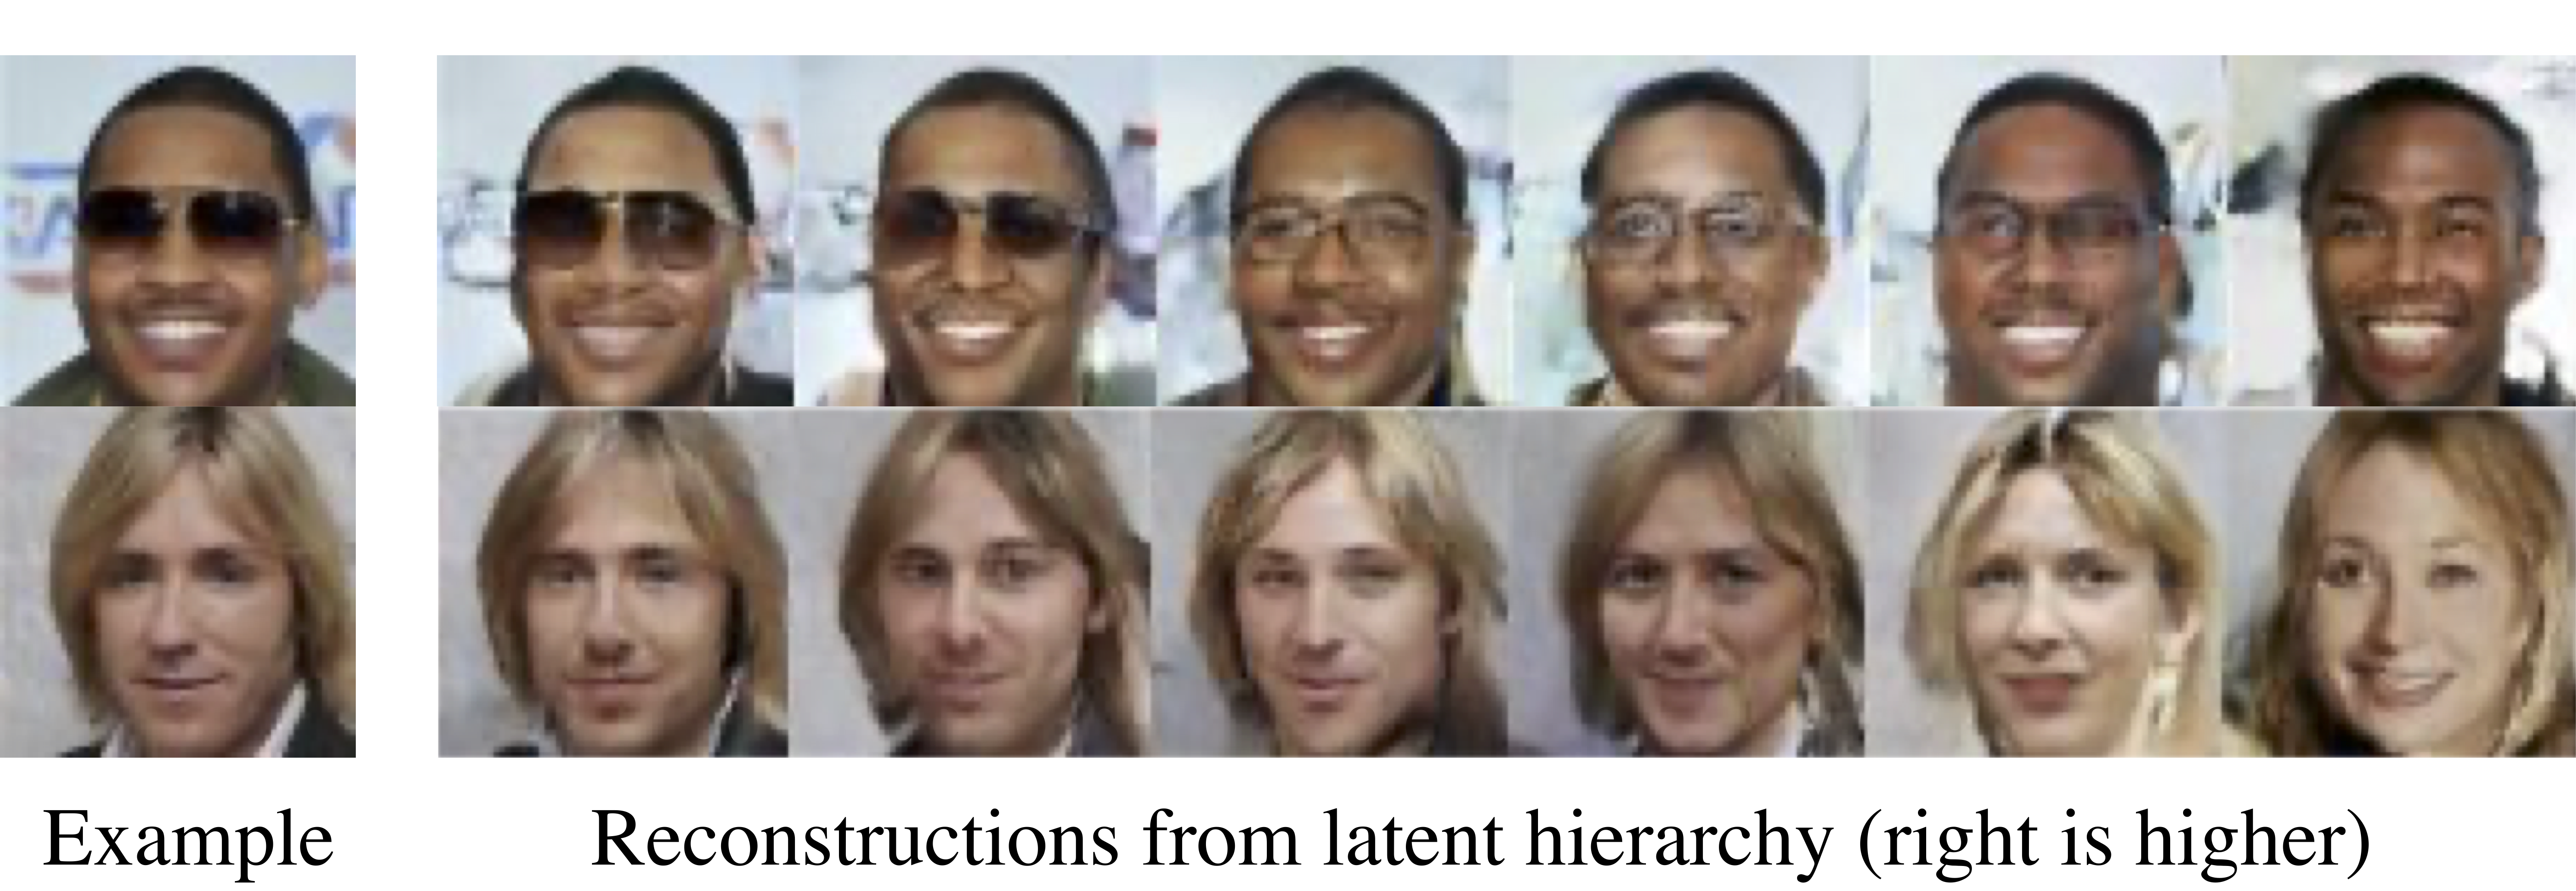
\includegraphics[width=1\columnwidth]{paper_hierarchical/biva_reconstructions.pdf}
    % https://docs.google.com/drawings/d/1UXdA3c18Oek9_env1vEB9mqOAHZ-tu0ijWmvqmapWCk/edit?usp=sharing
    \vspace{0mm}
    \caption[Reconstructions of in-distribution data (CelebA) of the BIVA model using higher latent variables.]{Reconstructions of in-distribution data (CelebA) of the BIVA model using higher latent variables  \parencite{maaloe_biva_2019}.
    The higher the latent variable, the more the reconstructions fall into the mode of the learned distribution.
    It is more common to wear regular glasses than sunglasses but most common not to wear glasses at all.
    A man with long hair collapses into the mode of the more common long-haired woman.}
    \vspace{0mm}
    \label{fig_hierarchical:biva-reconstructions-celeba}
\end{figure}
Finally, we look at reconstructions of out-of-distribution data.
\cref{fig_hierarchical:reconstructions-fashionmnist} illustrates that MNIST data is surprisingly well reconstructed by a hierarchical VAE trained on FashionMNIST.
Similar results have been found elsewhere \parencite{xiao_likelihood_2020}.
We repeat the previous experiment and replace inference distributions by their corresponding conditional prior, and now observe that reconstructions from higher latent layers become increasingly similar to the data on which the model was trained.
The reliance on conditional priors seems to prevent accurate reconstruction of out-of-distribution data.
Some details are lost on in-distribution data too, but the distinction between that and out-of-distribution data becomes more clear.

\textbf{These observations lead to our main hypothesis.}
The lowest latent variables in a hierarchical VAE learn generic features that can describe a wide range of data.
This enables the model to achieve high rates of compression and high likelihoods, even on out-of-distribution data as long as the learned low-level features are appropriate.
We further suggest that OOD data are in-distribution with respect to these low-level features, but not with respect to semantic ones.

\vspace{0cm}
\section{Background and related work}

\subsection{Variational autoencoders}
The variational autoencoder (VAE) \parencite{kingma_autoencoding_2014, rezende_stochastic_2014} is a framework for constructing deep generative models defined by an observed variable $\mathbf{x}$ and a stochastic latent variable $\mathbf{z}$.
Typically, a neural network with parameters $\thetab$ is chosen to parameterize the generative distribution $p_\thetab(\xb,\zb)=p_\thetab(\xb|\zb)p(\zb)$, where the prior $p(\zb)$ is commonly a standard Gaussian $\mathcal{N}(\0, \Ib)$.
The true posterior $p(\zb|\xb)$ is generally not analytically tractable and is approximated by a variational distribution $q_\phib(\zb|\xb)$ parameterized via another neural network with parameters $\phib$. The approximate posterior $q_\phib(\zb|\xb)$ is most often  a diagonal covariance Gaussian.
The model parameters $\thetab$ and variational parameters $\phib$ are jointly optimized by maximizing the \textit{evidence lower bound} (ELBO),
\begin{equation}\label{eq_hierarchical:elbo}
    \log p_\thetab(\xb) \geq \mathbb{E}_{q_\phib(\zb|\xb)} \left[ \log \frac{p_\thetab(\xb,\zb)}{q_\phib(\zb|\xb)} \right] \equiv \mathcal{L}(\xb; \thetab, \phib)\ .
\end{equation}
For brevity, we will denote $\mathcal{L}(\xb; \thetab, \phib)$ as $\mathcal{L}(\xb)$ or $\mathcal{L}$. The reparameterization trick is used to backpropagate gradients through the stochastic latent variables with low variance.

The VAE is defined with a single latent variable which limits the ability to learn a high likelihood representation of complex input distributions, e.g.\ natural images.
There exists a few complementary approaches to make the VAE more flexible: (i) model a more expressive variational distribution $q_\phib(\zb|\xb)$ or prior distribution $p_\thetab(\zb)$ \parencite{rezende_variational_2015, kingma_improved_2016}, (ii) model a more expressive posterior distribution $p_\thetab(\xb|\zb)$ e.g. with an autoregressive decoder \parencite{oord_conditional_2016} and (iii) learn a deeper hierarchy of latent variables \parencite{burda_importance_2016, sonderby_ladder_2016}.
Here, we focus on the latter.


\subsection{Hierarchical variational autoencoders}\label{sec_paper_hierarchical:background-hie-VAE}
Hierarchical VAEs are a family of probabilistic latent variable models which extends the basic VAE by introducing a hierarchy of $L$ latent variables $\zb=\zb_1, \dots, \zb_L$.
The most common generative model is defined from the top down as $p_\thetab(\xb|\zb)=p(\xb|\zb_1)p_\thetab(\zb_1|\zb_2)\cdots p_\thetab(\zb_{L-1}|\zb_L)$.
The inference model can then be defined in two ways respectively referred to as \textit{bottom-up} \parencite{burda_importance_2016}
\begin{equation}
    %q_\phib(\zb|\xb)=q_\phib(\zb_1|\xb)q_\phib(\zb_2|\zb_1)\cdots q_\phib(\zb_L|\zb_{L-1})
    q_\phib(\zb|\xb) = q_\phib(\zb_1|\xb)\textstyle\prod_{i=2}^{L} q_\phib(\zb_i|\zb_{i-1})
\end{equation}
and \textit{top-down} \parencite{sonderby_ladder_2016}
\begin{equation}
    % q_\phib(\zb|\xb)=q_\phib(\zb_{L}|\xb)q_\phib(\zb_{L-1}|\zb_L)\cdots q_\phib(\zb_2|\zb_1),
    q_\phib(\zb|\xb) = q_\phib(\zb_L|\xb)\textstyle\prod_{i=L-1}^{1} q_\phib(\zb_{i}|\zb_{i+1}) \ .
\end{equation}
Regardless of the choice of inference model, a hierarchical VAE is still trained using the ELBO \cref{eq_hierarchical:elbo}.

Until recently, hierarchical VAEs gave inferior likelihoods compared to state-of-the-art autoregressive \parencite{ho_flow_2019} and flow-based models \parencite{salimans_pixelcnn_2017}.
This was changed by \textcite{maaloe_biva_2019}, \textcite{vahdat_nvae_2020}, and \textcite{child_very_2021}, which introduced complementary methods to extend the number of latent variables to a very deep hierarchy resulting in state-of-the-art likelihood performance.

In this paper we employ a simple hierarchical VAE with bottom-up inference paths and the more powerful BIVA variant with a bidirectional (top-down and bottom-up) inference model \parencite{maaloe_biva_2019}. We employ skip connections between latent variables but omit them for brevity.


\subsection{Out-of-distribution detection}\label{sec_paper_hierarchical:background-ood-detection}
% Intro to alternative scores
So far, no reliable direct likelihood-based method has been found for fully unsupervised deep generative model OOD detection.
A major line of work considers developing new scores that are more reliable than the likelihood.
This includes the \textit{typicality} test presented by \textcite{nalisnick_detecting_2019} which is an OOD detection test based on the typicality of a batch of potentially OOD examples.
This approach however requires a batch of examples from the same class (OOD or not) which limits its practical applicability.
In \textcite{ren_likelihood_2019}, the \textit{likelihood ratio} between a primary model and a background model was shown to be an effective score for OOD detection.
However, to train the background model, the in-distribution data is perturbed via a data augmentation technique that is designed with knowledge about the confounding factors between the in-distribution data and the OOD data. Furthermore, it is tuned towards high performance on a known OOD dataset.
\textcite{serra_input_2020} take a similar approach and attribute the failure to detect OOD data to the high influence of the input complexity on the likelihood and choose a generic lossless compression algorithm as the background model.
Although this method gives good results, no single best choice of compression algorithm exists for all types of OOD data, and any particular choice encodes prior knowledge about the data into the detection method.
Both these methods can be seen as correcting for low-level features of the OOD data being assigned high model likelihood by using a second model focused exclusively on these features.

Similar to these methods, the majority of the approaches to OOD detection make assumptions about the nature of the OOD data.
The assumptions encompass using labels on the in-distribution data \parencite{hendrycks_baseline_2017, liang_enhancing_2018, alemi_uncertainty_2018, lee_simple_2018, lakshminarayanan_simple_2017}, examples of OOD data \parencite{hendrycks_deep_2019}, augmenting in-distribution data to mimic it \parencite{ren_likelihood_2019}, or assuming a certain data type \parencite{serra_input_2020}.
Any of these assumptions encode implicit biases into the model about the attributes of OOD data which, in turn, might impair performance on truly unknown data examples (unknown unknowns).

% Introduce the contrast to results with VAEs
While some of these methods achieve very good results on OOD detection with autoregressive models \parencite{oord_pixel_2016, salimans_pixelcnn_2017} and invertible flow-based models \parencite{kingma_glow_2018}, it was recently shown that they can be much less effective for VAEs \parencite{xiao_likelihood_2020} highlighting the need for a more reliable OOD score for VAEs.
Although VAEs have the same failure cases as autoregressive and flow-based models, the caveat is that the difference in the likelihood is generally not as big and reconstructions of OOD can be surprisingly good \parencite{xiao_likelihood_2020}.
\textcite{xiao_likelihood_2020} alleviate this by refitting the inference network, as previously proposed by \textcite{cremer_inference_2018, mattei_refit_2018}, to a potentially OOD example and measuring the so-called \textit{likelihood regret}.
However, refitting the inference network can be computationally expensive, especially for the large hierarchical VAEs that are used to model complex data \parencite{maaloe_biva_2019, vahdat_nvae_2020, child_very_2021}. Furthermore, this scales poorly to large amounts of potentially OOD examples as the optimization is done per example.

A few methods have approached OOD detection in a completely unsupervised fashion \parencite{maaloe_biva_2019, choi_waic_2019, xiao_likelihood_2020}.
The work of \textcite{maaloe_biva_2019} is the most related to ours. They introduce BIVA, a deep hierarchy of stochastic latent variables with a top-down and bottom-up inference model and achieve state-of-the-art likelihood scores. 
They also provide early results indicative that a looser likelihood bound may have value in OOD detection.
In this paper, we provide an explanation of those results, and significantly improve upon them.


\section{OOD detection with hierarchical VAEs}
\subsection{A bound for semantic OOD detection}
If the lowest latent variable in the VAE hierarchy codes for a large part of the low-level features required to reconstruct the input with high accuracy, as exemplified in \crefrange{fig_hierarchical:reconstructions-fashionmnist}{fig_hierarchical:biva-reconstructions-celeba}, then $p_\thetab(\xb|\zb_1)$ will be high for both in- and out-of-distribution data.
Hence, any OOD detection capabilities based on the ELBO $\mathcal{L} = \mathbb{E}_{q_\phib(\zb|\xb)}[\log p_\thetab(\xb|\zb_1)] - D_{\mathrm{KL}}( q_\phib(\zb|\xb) \parallel  p(\zb))$ from \cref{eq_hierarchical:elbo} relies on the KL-term for OOD detection. For a bottom-up hierarchical VAE, the KL-term $D_{\mathrm{KL}}( q_\phib(\zb|\xb) \parallel p(\zb))$ can be expressed by a hierarchical sum,% over the hierarchy
% \begin{multline}
%     \mathcal{L}(\xb) =  \mathbb{E}_{q_\phib(\zb|\xb)} \Big[ \log p_\thetab(\xb|\zb_1) \\
%                      + \textstyle\sum_{i=1}^{L-1} \log \frac{p_\thetab(\zb_i|\zb_{i+1})}{q_\phib(\zb_i|\zb_{i-1})} 
%                      + \log \frac{p_\thetab(\zb_L)}{q_\phib(\zb_L|\zb_{L-1})} \Big] .
% \end{multline}
% \begin{multline}
%     D_{\mathrm{KL}}( q(\zb|\xb) \parallel p(\zb)) = \\
%     \mathbb{E}_{q_\phib(\zb|\xb)} \Big[ \textstyle\sum_{i=1}^{L-1} \log \frac{p_\thetab(\zb_i|\zb_{i+1})}{q_\phib(\zb_i|\zb_{i-1})} + \log \frac{p_\thetab(\zb_L)}{q_\phib(\zb_L|\zb_{L-1})} \Big] .
% \end{multline}
\begin{equation}
    \mathbb{E}_{q_\phib(\zb|\xb)} \Big[ \textstyle\sum_{i=1}^{L-1} \log \frac{p_\thetab(\zb_i|\zb_{i+1})}{q_\phib(\zb_i|\zb_{i-1})} + \log \frac{p_\thetab(\zb_L)}{q_\phib(\zb_L|\zb_{L-1})} \Big] \ .
\end{equation}
In general, the absolute log-ratios grow with $\mathrm{dim}(\zb_i)$ as the individual log probability terms are computed by summing over the dimensionality of $\zb_i$.
This means that the value of the KL-term is dominated by terms where $\zb_i$ is high-dimensional. We refer to \cref{sec_hierarchical:analysis} for a more detailed argument.
Since hierarchical VAEs are generally constructed with a bottleneck type structure, the terms corresponding to latent variables towards the top of the hierarchy will have a vanishing influence on the value of the KL-term.
However, as the semantic information most relevant for OOD detection has a tendency to be represented in the top-most latent variables, this makes OOD detection using the regular ELBO difficult, even for state-of-the-art models.
This behavior has also been reported by \textcite{xiao_likelihood_2020}.

To shift the ELBO from primarily being based on the approximate posterior of the lowest latent variables to instead focus on the conditional prior, \textcite{maaloe_biva_2019} introduced slightly different likelihood lower bound defined as
\begin{equation}\label{eq_hierarchical:biva->k}
    \mathcal{L}^{>k} = \mathbb{E}_{p_\thetab(\zb_{\leq k}|\zb_{>k}) q_\phib(\zb_{>k}|\xb)} \left[ \log \frac{p_\thetab(\xb|\zb)p_\thetab(\zb_{>k})}{q_\phib(\zb_{>k}|\xb)} \right]
\end{equation}
where $k\in\{0,1,\dots,L\}$ (see \cref{sec_hierarchical:derivation_L_geq_k} for the derivation).
We note that $\mathcal{L}^{>0}$ is the regular ELBO (\cref{eq_hierarchical:elbo}) and that empirically we always observe that $\mathcal{L}\geq\mathcal{L}^{>k} \, \forall \, k$ although this need not hold in general.
The core idea behind this variation on the ELBO is to sample the $k$ lowest latent variables from the conditional prior $\zb_1,\dots,\zb_l \sim p_\thetab(\zb_{\leq k}|\zb_{>k})$ and only the $L-k$ highest from the approximate posterior $\zb_{k+1},\dots,\zb_L \sim q_\phib(\zb_{>k}|\xb)$.
Importantly, this has the effect that the data likelihood $p(\xb|\zb)$ is dependent on the approximate posterior through a latent variable $\zb_{k+1}$ different from $\zb_1$ for all $k \geq 1$.
Thereby, the likelihood can be evaluated with a reconstruction from each of the latent variables $\zb_k$ of the hierarchical VAE.
Hence, we can now test how well the input $\xb$ is reconstructed from each latent variable.
The notation $\mathcal{L}^{>k}$ highlights that for latent variables $\zb_{>k}$, the bound is the regular ELBO while for the latent variables $\zb_{\leq k}$, the bound is evaluated using the (conditional) prior rather than the approximate posterior as the proposal distribution.


\subsection{A likelihood-ratio score for all feature levels}
While the $\mathcal{L}^{>k}$ bound provides a score for performing semantic OOD detection, it still relies on the data space likelihood function (see equation \cref{eq_hierarchical:likelihoods-as-exact} below), which is known to be problematic for OOD detection (\cref{sec_paper_hierarchical:background-ood-detection}). To alleviate this, we phrase OOD detection as a likelihood ratio test of being \emph{semantically} in-distribution.
A standard likelihood ratio test \parencite{buse_likelihood_1982} suggests considering the ratio between the associated likelihoods, which we can approximate on a log-scale by the corresponding lower bounds $\mathcal{L}$ and $\mathcal{L}^{>k}$,
\begin{equation}\label{eq_hierarchical:llr-as-difference-in-likelihoods}
    % LLR = - 2 log(L0 / L1)
    % where L0 < L1 so log(L0 / L1) < 0 and LLR > 0
    % LLR = 2 log(L1 / L0)
    %     = 2 (log(L1) - log(L0))
    %     = 2 (ELBO - L^{>k})  % LLR^{>a,>b} where a=0
    % L1 = ELBO
    % L0 = L^{>k}
    LLR^{>k}(\xb) = \mathcal{L}(\xb) - \mathcal{L}^{>k}(\xb) \ .
\end{equation}
%This likelihood ratio contrasts the ELBO with $\mathcal{L}^{>k}$ for a variable choice of $k$.
Since, empirically, $\mathcal{L}\geq\mathcal{L}^{>k}$, the ratio is always positive as is standard for likelihood ratio tests.
A low value of $LLR^{>k}(\xb)$ means that the ELBO and $\mathcal{L}^{>k}$ are almost equally tight for the data.
On the contrary, a high value indicates that $\mathcal{L}^{>k}$ is looser on the data than the ELBO; hence, the data may be OOD.


We can gather further insights about this score if we write the regular ELBO and the $\mathcal{L}^{>k}$ bounds in the exact form that includes the intractable KL-divergence between the approximate and true posteriors,
\begin{align}
    \mathcal{L}      &= \log p_\thetab(\xb) - D_{\mathrm{KL}}\left( q_\phib(\zb|\xb) \parallel p_\thetab(\zb|\xb)\right), \label{eq_hierarchical:likelihoods-as-exact} \\ 
    \mathcal{L}^{>k} &= \log p_\thetab(\xb) - D_{\mathrm{KL}}\left( p_\thetab(\zb_{\leq k }|\zb_{>k}) q_\phib(\zb_{>k}|\xb) \parallel p_\thetab(\zb|\xb)\right) \nonumber \ .
\end{align}
Subtracting these cancel out the two data likelihood terms $\log p_\thetab(\xb)$ and only the KL-divergences from the approximate to the true posterior remain,
\begin{align}
    LLR^{>k}(\xb) &= - D_{\mathrm{KL}}\left( q_\phib(\zb|\xb) \parallel p_\thetab(\zb|\xb)\right) \\
                 &\quad + D_{\mathrm{KL}}\left( p_\thetab(\zb_{\leq k}|\zb_{>k}) q_\phib(\zb_{>k}|\xb) \parallel p_\thetab(\zb|\xb)\right) \ . \notag
\end{align}\label{eq_hierarchical:llr-as-kls}

Hence, it is clear that compared to the likelihood bound $\mathcal{L}^{>k}$, this likelihood-ratio measures divergence exclusively in the latent space whereas $\mathcal{L}^{>k}$ includes the $\log p_\thetab(\xb)$ term similar to the ELBO.
Therefore, the $LLR^{>k}$ score should be an improved method for semantic OOD detection compared to $\mathcal{L}^{>k}$.
Now, it can be noted that if we replace the regular ELBO, $\mathcal{L}$, in \cref{eq_hierarchical:likelihoods-as-exact} with the strictly tighter importance weighted bound \parencite{burda_importance_2016},
\begin{equation}
    \mathcal{L}_{S} = \mathbb{E}_{q(\zb|\xb)}\left[ \log \frac{1}{N} \sum_{s=1}^{S} \frac{p(\xb, \zb^{(s)})}{q(\zb^{(s)}|\xb)} \right] \ , \label{eq_hierarchical:iw-bound}
\end{equation}
then, in the limit $S\rightarrow\infty$, we have $\mathcal{L}_{S} \rightarrow \log p_\thetab(\xb)$ and the likelihood ratio reduces to
\begin{equation}
    LLR^{>k}_{S}(\xb) \rightarrow D_{\mathrm{KL}}( p(\zb_{\leq k}|\zb_{>k}) q(\zb_{>k}|\xb) \parallel p(\zb|\xb))
\end{equation}\label{eq_hierarchical:llr-as-kls-iwae-reduced}
which, in practice, is well-approximated for a finite $S$. We expect this importance weighted likelihood ratio to monotonically improve upon the one in \cref{eq_hierarchical:llr-as-kls} as $S$ increases and the KL-divergence in the regular ELBO that contains terms for which $\zb_i$ is high-dimensional goes to zero.


Since the scores in \cref{eq_hierarchical:llr-as-kls,eq_hierarchical:llr-as-kls-iwae-reduced} are estimated by sampling their estimators are stochastic objects with nonzero variance.
We note that $\text{Var}(\widehat{LLR}^{>k}) = \text{Var}(\hat{\mathcal{L}}) + \text{Var}(\hat{\mathcal{L}}^{>k}) - 2\, \text{Cov}(\hat{\mathcal{L}}, \hat{\mathcal{L}}^{>k})$.
Since $\log p_\thetab(\xb)$ and part of the KL-divergence are identical in the expressions of $\mathcal{L}$ and $\mathcal{L}^{>k}$ we expect $\text{Cov}(\hat{\mathcal{L}}, \hat{\mathcal{L}}^{>k})$ to be positive which reduces the total variance. 
Empirical results indeed show that $\text{Var}(\widehat{LLR}^{>k})$ is larger than $\text{Var}(\hat{\mathcal{L}})$ but smaller than $\text{Var}(\hat{\mathcal{L}}^{>k})$.
%Whether this decreases the variance to below the variance of any of the two bounds, we do not know, and we believe it to be difficult to verify mathematically.
Nevertheless, the variance of the estimators is guaranteed to go to zero as the number of samples is increased.

The OOD scores considered in this research all assume that what discriminates an out-of-distribution from an in-distribution data point are semantic, high-level features. Clearly, if this is not the case and the difference instead lies in low-level statistics, the scores would likely fail. We hypothesize that a complementary bound to \cref{eq_hierarchical:biva->k}, $\mathcal{L}^{<l}$ described in \cref{sec_hierarchical:complementary-bound}, might be useful in these cases, but leave further examination to future work.


\section{Experimental setup}

\paragraph{Tasks} We follow existing literature \parencite{nalisnick_deep_2019, hendrycks_deep_2019} and evaluate our method by setting up OOD detection tasks from FashionMNIST \parencite{xiao_fashionmnist_2017} to MNIST \parencite{lecun_gradientbased_1998} and from CIFAR10 \parencite{krizhevsky_learning_2009} to SVHN \parencite{netzer_reading_2011}.
For each experiment we train our model on the train split of the former dataset and test its ability to recognize the test split of the latter dataset as OOD from the test split of the former dataset.
We use the standard train/test splits for the datasets.
More details on the datasets can be found in the \cref{sec_hierarchical:datasets}.


% Our model
%\begin{wrapfigure}{R}{0.5\columnwidth}
% \begin{SCfigure}[50][t!]
\begin{figure}
    %\begin{figure}
    \centering
    \resizebox{0.25\textwidth}{!}{
    \tikz{
        % inference
        % nodes
        \node[obs] (x_inf) {$\xb$};
        \node[latent,above=.75cm of x_inf](z1_inf){$\zb_1$};
        \node[latent,above=.75cm of z1_inf](z2_inf){$\zb_2$};
        % \node[latent,above=.75cm of z2_inf](z3_inf){$\zb_3$};
        \node[above=of z2_inf, yshift=-1.cm] (phi) {$q_\phib(\zb|\xb)$};
        
        % edges
        \edge[]{x_inf}{z1_inf}; %
        \edge[]{z1_inf}{z2_inf}; %
        % \edge[]{z2_inf}{z3_inf}; %
        \edge[dashed, bend left]{x_inf}{z2_inf}; %
        % \edge[dashed, bend left]{x_inf}{z3_inf}; %
        
        % generative
        % nodes$
        \node[obs,right=0.75cm of x_inf] (x_gen) {$\xb$};
        \node[latent,above=.75cm of x_gen](z1_gen){$\zb_1$};
        \node[latent,above=.75cm of z1_gen](z2_gen){$\zb_2$};
        % \node[latent,above=.75cm of z2_gen](z3_gen){$\zb_3$};
        \node[above=of z2_gen, yshift=-1.cm] (theta) {$p_\thetab(\xb,\zb)$};
        
        % edges
        % \edge[]{z3_gen}{z2_gen}; %
        \edge[]{z2_gen}{z1_gen}; %
        \edge[]{z1_gen}{x_gen}; %
        \edge[dashed, bend left]{z2_gen}{x_gen}; %
        % \edge[dashed, bend left]{z3_gen}{x_gen}; %
    }
    }
    \caption[Inference and generative models for a bottom-up hierarchical VAEs.]{ The inference and generative models, $q_\phib$ and $p_\thetab$, for an $L=2$ layered bottom-up hierarchical VAE as the one used in our experiments.
    Dashed lines indicate deterministic skip connections which are employed in both networks. Skip connections are found to be useful for optimizing latent variable models \parencite{dieng_avoiding_2019, maaloe_biva_2019}.}
    \label{fig_hierarchical:hvae-graphical-model}
    % \end{figure}
%\end{wrapfigure}
% \end{SCfigure}
\end{figure}


\paragraph{Models} For each OOD task, we train a simple bottom-up hierarchical VAE with $L$ stochastic layers which we will refer to as ``HVAE''.
To alleviate posterior collapse we include skip-connections that connect $\zb_i$ to $\zb_{i+2}$ for $i\in\{0, L-2\}$ and $\zb_0\equiv\xb$ in both the inference and generative models \parencite{dieng_avoiding_2019} and employ the \textit{free bits} scheme with $\lambda=2$ \parencite{kingma_improved_2016}.
We use weight-normalization \parencite{salimans_weight_2016} on all weights and residual networks in the deterministic paths. 
A graphical representation of this model can be seen in \cref{fig_hierarchical:hvae-graphical-model}.
We use a Bernoulli output distribution for FashionMNIST/MNIST and a discretized mixture of logistics output distribution \parencite{salimans_pixelcnn_2017} for CIFAR10/SVHN.
We use $L=3$ for grayscale images and $L=4$ for natural images.
% For CIFAR/SVHN, we also train a BIVA model \parencite{maaloe_biva_2019} with $L=10$ and similar configuration as used by the original paper\footnote{Code available at \url{github.com/larsmaaloee/BIVA} and \url{github.com/vlievin/biva-pytorch}}.
Full model details are in the \cref{sec_hierarchical:model-details}.


% Baselines
\paragraph{Baselines} We group baselines into those that use prior knowledge about OOD data, ones that use labels associated with the in-distribution data and purely unsupervised approaches that do not make such assumptions.
Our method falls into the latter category.
For more information on each baseline, we refer to the original literature.


% Metrics and Evaluation
\paragraph{Evaluation} Following previous work \parencite{hendrycks_baseline_2017, hendrycks_deep_2019, alemi_uncertainty_2018, ren_likelihood_2019, choi_waic_2019} we use the threshold-independent evaluation metrics of Area Under the Receiver Operator Characteristic (AUROC$\uparrow$), Area Under the Precision Recall Curve (AUPRC$\uparrow$) and False Positive Rate at 80\% true positive rate (FPR80$\downarrow$) where the arrow indicates the direction of improvement.
Note that these metrics are only computable given examples of OOD data but faced with truly OOD data (unknown unknowns), there are many ways to select thresholds to use in practice e.g.\ as the one that yields a specific tolerable false positive rate on the in-distribution test data.
To compute the metrics, we use an equal number of samples from the in-distribution and OOD datasets by including all examples in the smallest of the two sets and randomly sampling equally many from the larger. We compute the $LLR^{>k}$ score with one and $S$ importance samples denoted by $LLR^{>k}_S$.

% The value of k
\paragraph{Selection of $k$} To determine whether an example is OOD in practice, the value of $LLR^{>k}$ is computed on the in-distribution test set for all $k$ and the resulting empirical distribution is used as reference.
If for any value of $k$, the $LLR^{>k}$ score of a new input differs significantly from the empirical distribution, it is regarded OOD.
If it differs for multiple values of $k$, the value for which it differs the most is selected.
In our experiments, we consider an entire dataset at a time and report the results of $LLR^{>k}$ with the value of $k$ that yielded the highest AUROC$\uparrow$ for that dataset in a threshold-free manner.
In practice, slightly better performance may be achieved by choosing $k$ per example.
This would not exclude the use of batching in our method, since $LLR^{>k}$ is computed after the forward pass.


\section{Results}

The likelihoods for our trained models are in \cref{tab_hierarchical:bits-per-dim-ood} alongside baseline results for in-distribution and OOD data.
The main results of the paper on the OOD tasks can be seen along with comparisons to the baseline methods in \cref{tab_hierarchical:rocauc-ood}.
We note that for all our results, the value of the score ($\mathcal{L}^{>k}$ and $LLR^{>k}$) for the training and test splits of the in-distribution data was observed to have the same empirical distribution to within sampling error hence yielding an AUROC score of $\approx0.5$ as expected.
Results on additional commonly used datasets are found in \cref{sec_hierarchical:additional-results}.


\begin{table}
    \caption[Average bits per dimension of different datasets for generative models trained on FashionMNIST and CIFAR10.]{ Average bits per dimension of different datasets for models trained on FashionMNIST and CIFAR10.
    For the hierarchical models we include the $\mathcal{L}^{>k}$ bounds.
    The likelihoods of training and test splits of the in-distribution data are all cases close.
    Since we train on dynamically binarized FashionMNIST, our bits/dim are smaller than for Glow.
    As $k$ is increased for the $L^{>k}$ bound, the bound gets looser, but the model eventually assigns higher likelihood to the in distribution data than to the OOD data.
    Glow refers to \textcite{kingma_glow_2018, nalisnick_deep_2019}.
    BIVA refers to our implementation of \textcite{maaloe_biva_2019}.}
    \centering
    \resizebox{0.8\columnwidth}{!}{%
    \begin{tabular}{lrrrrr}
        \toprule
         Method & Dataset & \multicolumn{4}{c}{Avg. bits/dim}\\
        %   & & $\log p(x)$ & $\mathcal{L}^{>k_1}$ & $\mathcal{L}^{>k_2}$ & $\mathcal{L}^{>k_3}$\\
          & & $\log p(x)$ & $\mathcal{L}^{>1}$ & $\mathcal{L}^{>2}$ & $\mathcal{L}^{>3}$\\
         \midrule
         \multicolumn{6}{c}{\textbf{Trained on FashionMNIST}} \\
         \midrule
         \multirow{2}{*}{Glow}
            & FashionMNIST & 2.96 & - & - & \\
            & MNIST & 1.83 & - & - & \\
         \multirow{2}{*}{HVAE (Ours)}
            & FashionMNIST & 0.420 & 0.476 & 0.579 & - \\
            & MNIST & 0.317 & 0.601 & 0.881 & - \\
         \midrule
         \multicolumn{6}{c}{\textbf{Trained on CIFAR10}} \\
         \midrule
         \multirow{2}{*}{Glow}
          & CIFAR10 & 3.46 & - & - & \\
          & SVHN & 2.39 & - & - & \\
         \multirow{2}{*}{HVAE (Ours)}
            & CIFAR10 & 3.74 & 17.8 & 54.3 & 75.7 \\  % log p(x) = 8010.03
            & SVHN & 2.62 & 10.2 & 64.0 & 93.9 \\
         \multirow{2}{*}{BIVA (Ours)}
          & CIFAR10 & 3.46 & 8.74 & 19.7 & 37.3 \\
          & SVHN & 2.35 & 6.62 & 25.1 & 59.0 \\
         \bottomrule
    \end{tabular}
    }
    \label{tab_hierarchical:bits-per-dim-ood}
    \vspace{0mm}
\end{table}


\todo[inline]{Check out if we can make underbrace like curly brackets to the left of tab_hierarchical:rocauc-ood to decrease height and fit page better.}
\begin{table}
    \caption[AUROC, AUPRC, and FPR80 of generative models for OOD detection (MNIST/FashionMNIST and SVHN/CIFAR10).]{%
        AUROC$\uparrow$, AUPRC$\uparrow$ and FPR80$\downarrow$ for OOD detection for a FashionMNIST model using scores on the FashionMNIST test set as reference. We bold the best results within the "No OOD-specific assumptions" group since we only compare directly to those.
        HVAE (ours) refers to our hierarchical bottom-up VAE.
        BIVA (ours) refers to our implementation of the hierarchical BIVA model.
    }
    \centering
    \resizebox*{!}{0.83\textheight}{%
    \begin{tabular}{lrrr}
        \toprule
         Method & AUROC$\uparrow$ & AUPRC$\uparrow$ & FPR80$\downarrow$ \\
         \midrule
         \multicolumn{4}{c}{\textbf{FashionMNIST (in) / MNIST (out)}} \\
         \midrule
         \multicolumn{4}{l}{\textbf{Use prior knowledge of OOD}} \\
Backgr. contrast. LR (PixelCNN) {\parencite{ren_likelihood_2019}}               & $0.994$ & $0.993$ & $0.001$ \\
Backgr. contrast. LR (VAE) {\parencite{choi_waic_2019}}                    & $0.924$ & - & - \\
Binary classifier {\parencite{ren_likelihood_2019}}                              & $0.455$ & $0.505$ & $0.886$ \\ % 6
$p(\hat{y} | \xb)$ with OOD as noise class {\parencite{ren_likelihood_2019}}     & $0.877$ & $0.871$ & $0.195$ \\ % 7
$p(\hat{y} | \xb)$ with calibration on OOD {\parencite{ren_likelihood_2019}}     & $0.904$ & $0.895$ & $0.139$ \\ % 8
Input complexity ($S$, Glow) \parencite{hendrycks_deep_2019}                    & $0.998$ & - & - \\
Input complexity ($S$, PixelCNN++) \parencite{hendrycks_deep_2019}              & $0.967$ & - & - \\
         \multicolumn{4}{l}{\textbf{Use in-distribution data labels $y$}} \\
$p(\hat{y} | \xb)$ {\parencite{ren_likelihood_2019, hendrycks_baseline_2017}}                        & $0.734$ & $0.702$ & $0.506$ \\
Entropy of $p(y | \xb)$ {\parencite{ren_likelihood_2019}}                        & $0.746$ & $0.726$ & $0.448$ \\
ODIN {\parencite{ren_likelihood_2019, liang_enhancing_2018}}                                       & $0.752$ & $0.763$ & $0.432$ \\
VIB \parencite{alemi_uncertainty_2018, choi_waic_2019}                                          & $0.941$ & - & - \\
Mahalanobis distance, CNN {\parencite{ren_likelihood_2019}}                     & $0.942$ & $0.928$ & $0.088$ \\
Mahalanobis distance, DenseNet {\parencite{lee_simple_2018}}                & $0.986$ & - & - \\
Ensemble, 20 classifiers {\parencite{ren_likelihood_2019, lakshminarayanan_simple_2017}}                  & $0.857$ & $0.849$ & $0.240$ \\
         \multicolumn{4}{l}{\textbf{No OOD-specific assumptions}} \\
         \multicolumn{4}{l}{\textit{- Ensembles}} \\
WAIC, 5 models, VAE {\parencite{choi_waic_2019}}                          & $0.766$ & - & - \\
WAIC, 5 models, PixelCNN {\parencite{ren_likelihood_2019}}                      & $0.221$ & $0.401$ & $0.911$ \\
        \multicolumn{4}{l}{\textit{- Not ensembles}} \\
Likelihood regret \parencite{xiao_likelihood_2020}                               & $\mathbf{0.988}$ & - & - \\
$\mathcal{L}^{>0}$ + HVAE (ours)                    & $0.268$ & $0.363$ & $0.882$ \\
$\mathcal{L}^{>1}$ + HVAE (ours)                    & $0.593$ & $0.591$ & $0.658$ \\
$\mathcal{L}^{>2}$ + HVAE (ours)                    & $0.712$ & $0.750$ & $0.548$ \\
$LLR^{>1}$ + HVAE (ours)                            & $0.964$ & $0.961$ & $0.036$ \\
$LLR^{>1}_{250}$ + HVAE (ours)                      & $0.984$ & $\mathbf{0.984}$ & $\mathbf{0.013}$ \\
         \midrule
         \multicolumn{4}{c}{\textbf{CIFAR10 (in) / SVHN (out)}} \\
         \midrule
         \multicolumn{4}{l}{\textbf{Use prior knowledge of OOD}} \\
Backgr. contrast. LR (PixelCNN) {\parencite{ren_likelihood_2019}}               & $0.930$ & $0.881$ & $0.066$ \\
Backgr. contrast. LR (VAE) {\parencite{xiao_likelihood_2020}}                    & $0.265$ & - & - \\
Outlier exposure {\parencite{hendrycks_deep_2019}}                              & $0.984$ & - & - \\
Input complexity ($S$, Glow) \parencite{serra_input_2020}                   & $0.950$ & - & - \\
Input complexity ($S$, PixelCNN++) \parencite{serra_input_2020}             & $0.929$ & - & - \\
Input complexity ($S$, HVAE) (Ours) \parencite{serra_input_2020}\textsuperscript{\ref{footnote:serra_hierarchical_likelihood}} & $0.833$ & $0.855$ & $0.344$ \\
% Input complexity ($S$, HVAE) (Ours) \parencite{serra_input_2020}\% \footnote{\textcite{serra_input_2020} performs the best when high likelihoods are assigned to OOD data such that the overlap with in-distribution data is low. Performance is worse when the overlap is high, cf. \textcite[Table 1]{serra_input_2020}, as seen with complex images.} & $0.833$ & $0.855$ & $0.344$ \\
\multicolumn{4}{l}{\textbf{Use in-distribution data labels $y$}} \\
Mahalanobis distance {\parencite{lee_simple_2018}}                          & $0.991$ & - & -  \\
         \multicolumn{4}{l}{\textbf{No OOD-specific assumptions}} \\
         \multicolumn{4}{l}{\textit{- Ensembles}} \\
WAIC, 5 models, Glow {\parencite{choi_waic_2019}}                          & $1.000$ & - & - \\
WAIC, 5 models, PixelCNN {\parencite{ren_likelihood_2019}}                      & $0.628$ & $0.616$ & $0.657$ \\
         \multicolumn{4}{l}{\textit{- Not ensembles}} \\
Likelihood regret \parencite{xiao_likelihood_2020}                               & $0.875$ & - & - \\
$LLR^{>2}$ + HVAE (ours)                            & $0.811$ & $0.837$ & $0.394$ \\
$LLR^{>2}$ + BIVA (ours)                            & $\mathbf{0.891}$ & $\mathbf{0.875}$ & $\mathbf{0.172}$ \\
         \bottomrule
    \end{tabular}%
    }
    \label{tab_hierarchical:rocauc-ood}
\end{table}

\addtocounter{footnote}{1}
\footnotetext{
    \textcite{serra_input_2020} performs the best when high likelihoods are assigned to OOD data such that the overlap with in-distribution data is low.
    Performance is worse when the overlap is high, cf. \textcite[Table 1]{serra_input_2020}, as seen with complex images.
    \label{footnote:serra_hierarchical_likelihood}
}



\subsection{Likelihood-based OOD detection}
% \begin{sidewaysfigure}
\begin{figure}
    %\captionstyle{centerlast}
    \centering
    \begin{subfigure}[l]{0.48\columnwidth}
        \centering
        \includegraphics[width=1\columnwidth]{paper_hierarchical/densities-FashionMNIST-test-MNIST-test-bpp-k-0_sohau.pdf}
        \caption{}
        \label{fig_hierarchical:FMNIST-elbo-k0}
    \end{subfigure}
    % \hfill
    \begin{subfigure}[c]{0.48\columnwidth}
        \centering
        \includegraphics[width=1\columnwidth]{paper_hierarchical/densities-FashionMNIST-test-MNIST-test-bpp-k-2_sohau.pdf}
        \caption{}
        \label{fig_hierarchical:FMNIST-elbo-k2}
    \end{subfigure}
    % \hfill
    \begin{subfigure}[r]{0.48\columnwidth}
        \centering
        \includegraphics[width=1\columnwidth]{paper_hierarchical/densities-FashionMNIST-test-MNIST-test-LLR-0-1_sohau.pdf}
        \caption{}
        \label{fig_hierarchical:FMNIST-llr}
    \end{subfigure}
    \caption[Empirical densities of FashionMNIST (in-distribution) and MNIST (OOD) using the raw likelihood and $\mathcal{L}^{>2}$ bound.]{%
    Empirical densities of FashionMNIST (in-distribution) and MNIST (OOD) using the raw likelihood \subref{fig_hierarchical:FMNIST-elbo-k0}, the $\mathcal{L}^{>2}$ bound \subref{fig_hierarchical:FMNIST-elbo-k2} and the $LLR^{>1}$ score \subref{fig_hierarchical:FMNIST-llr}. All densities are computed using the HVAE model.
    For the regular likelihood MNIST is very clearly more likely on average than the FashionMNIST test data while with the $\mathcal{L}^{>2}$ bound separation is better but significant overlap remains.
    The $LLR^{>1}$ provides a high degree of separation. Likelihoods are reported in units of the natural log of the number of bits per dimension.
    }
    \label{fig_hierarchical:FMNIST-ood-densities}
\end{figure}
% \end{sidewaysfigure}

We first report the results of the different variations of the $\mathcal{L}^{>k}$ bound for OOD detection. 
We reconfirm the results of \textcite{nalisnick_deep_2019} by observing that our hierarchical latent variable models also assign higher $\mathcal{L}^{>0}$ to the OOD dataset in the FashionMNIST/MNIST and CIFAR10/SVHN cases resulting in an AUROC$\uparrow$ inferior to random (\cref{tab_hierarchical:rocauc-ood}).
Switching the in-distribution data for the OOD data in both cases result in correctly detecting the OOD data; an asymmetry also reported by \textcite{nalisnick_deep_2019}.
\cref{fig_hierarchical:FMNIST-elbo-k0} shows the density of $\mathcal{L}^{>0}$ in bits per dimension \parencite{theis_note_2016} by the model trained on FashionMNIST when evaluated on the FashionMNIST and MNIST test sets.
We observe a high degree of overlap, with less separation of the OOD data compared to similar results of autoregressive and flow-based models, like \textcite{xiao_likelihood_2020}.


We then evaluate the looser $\mathcal{L}^{>k}$ \cref{eq_hierarchical:biva->k} for $k\in\{1,L\}$.
\cref{fig_hierarchical:FMNIST-elbo-k2} shows the result for $\mathcal{L}^{>2}$, which yielded the highest AUCROC$\uparrow$, only slightly better than random.
Like \textcite{maaloe_biva_2019}, we see that increasing the value of $k$ generally leads to improved OOD detection.
However, we also observe that the two empirical distributions never cease to overlap.
Importantly, depending on the OOD dataset, the amount of remaining overlap can be high which limits the discriminatory power of the likelihood-based $\mathcal{L}^{>k}$ bound.
This is in-line with the pathological behavior of the raw likelihood of latent variable models when used for OOD detection \parencite{xiao_likelihood_2020}.
Since a high degree of overlap also seems present in \textcite{maaloe_biva_2019}, and we see the same problem for our BIVA model trained on CIFAR10, we do not expect this to be due to the less expressive HVAE.


\subsection{Likelihood-ratio-based OOD detection}

We now move to the likelihood ratio-based score.
We find that $LLR^{>k}$ separates the OOD MNIST data from in-distribution FashionMNIST to a higher degree than the likelihood estimates as can be seen by the empirical densities of the score in \cref{fig_hierarchical:FMNIST-llr}.
We note that the likelihood ratio between the ELBO and the $\mathcal{L}^{>k}$ bound provides the highest degree of separation of MNIST and FashionMNIST as measured by the AUROC$\uparrow$ for $k=1$ smaller than $L$.
This is not surprising since the value of $k$ that provides the maximal separation to the reference in-distribution dataset need not be the one for which $\mathcal{LLR}^{>k}$ is overall maximal for the OOD dataset.
We also visualize the ROC curves resulting from using the $LLR^{>k}$ score for OOD detection on both FashionMNIST/MNIST and CIFAR10/SVHN and compare it to the ROC curves resulting from the different $\mathcal{L}^{>k}$ bounds in \cref{fig_hierarchical:FMNIST-roc-llr and CIFAR10-roc-llr}, respectively.
On both datasets we see significantly better discriminatory performance when using the $LLR^{>k}$ score.

\cref{tab_hierarchical:rocauc-ood} shows that BIVA improves upon the HVAE model for OOD detection on CIFAR while \cref{tab_hierarchical:bits-per-dim-ood} shows that the BIVA model also improves upon the HVAE in terms of likelihood.
We hypothesize that models larger than our implementation of BIVA, with better likelihood scores may perform even better \parencite{maaloe_biva_2019, vahdat_nvae_2020, child_very_2021}.

\begin{figure}
    \centering
    \begin{subfigure}[l]{0.495\columnwidth}
        \includegraphics[width=1\columnwidth]{paper_hierarchical/roc-FashionMNIST-test-MNIST-test-ll-and-llr-IW250_sohau.pdf}
        % \caption{}
        % \caption{ROC curves with AUROC score for detecting MNIST as OOD with the HVAE model trained on FashionMNIST.
        % A ROC curve is plotted for each of the $\mathcal{L}^{>k}$ bounds including the ELBO along with one for the best-performing log likelihood-ratio $LLR^{>1}$.}
        % \label{fig_hierarchical:FMNIST-roc-llr}
    \end{subfigure}
    \hfill
    \begin{subfigure}[r]{0.495\columnwidth}
        \includegraphics[width=1\columnwidth]{paper_hierarchical/roc-biva-CIFAR10-SVHN-ll-and-llr_sohau.pdf}
        % \caption{}
        % \caption{ROC curves with AUROC score for detecting SVHN as OOD with the BIVA model trained on CIFAR10.
        % A ROC curve is plotted for each of the $\mathcal{L}^{>k}$ bounds including the ELBO along with one for the best-performing log likelihood-ratio $LLR^{>2}$.}
        % \label{fig_hierarchical:CIFAR10-roc-llr}
    \end{subfigure}
    \caption[ROC curves for out of distribution detection (MNIST/FashionMNIST and SVHN/CIFAR10).]{%
        ROC curves with AUROC score for detecting MNIST as OOD with the HVAE model trained on FashionMNIST (left) and SVHN as OOD with the BIVA model trained on CIFAR10 (right). 
        A ROC curve is plotted for each of the $\mathcal{L}^{>k}$ bounds including the ELBO along with one for the best-performing log likelihood-ratio $LLR^{>1}$.
    }
    \label{fig_hierarchical:FMNIST-roc-llr and CIFAR10-roc-llr}
\end{figure}


\subsection{Comparison to baselines}
\paragraph{Performance} \cref{tab_hierarchical:rocauc-ood} summarize our results compared to baselines based on the commonly used AUROC$\uparrow$, AUPRC$\uparrow$ and FPR80$\downarrow$ metrics.
Our method outperforms other generative model-based methods such as WAIC \parencite{choi_waic_2019} with Glow model and performs similarly to the likelihood regret method of \parencite{xiao_likelihood_2020}.
Furthermore, our method performs similarly to the background contrastive likelihood ratio method of \textcite{ren_likelihood_2019} on FashionMNIST/MNIST but contrary to the failure of that method on CIFAR10/SVHN reported by \parencite{xiao_likelihood_2020}, our method performs very well on this task too.
Our approach outperforms all supervised approaches that use in-distribution labels or synthetic examples of OOD data derived from the in-distribution data including ODIN \parencite{liang_enhancing_2018} and the predictive distribution of a classifier $p(\hat{y}|\xb)$ trained and evaluated in various ways (see \textcite{ren_likelihood_2019}).

\paragraph{Runtime} For a full evaluation of a single example across all feature levels of a model with $L$ stochastic layers, our method requires $L-1$ forward passes through the inference and generative networks as well as computing the likelihood ratio, of which the forward passes are dominant.
For a typical forward pass that is linear in the input dimensionality, $D$, and the number of stochastic layers, $L$, this amounts to computation of $\mathcal{O}(DL)$.
Compared to some related work that either requires an $M>1$ sized batch of inputs of which either all or none are OOD \parencite{nalisnick_detecting_2019} or cannot be applied to batches due to the required per-example optimization \parencite{xiao_likelihood_2020}, our method additionally is applicable to batches of any size that may consist of both OOD and in-distribution examples which provides drastic speed-ups via vectorization and parallelization.
Furthermore, the method of \textcite{xiao_fashionmnist_2017} requires refitting the inference network of a VAE which can be computationally demanding.
Compared to the likelihood ratio proposed in \textcite{ren_likelihood_2019}, our method requires training only a single model on a single dataset.


\section{Discussion}
Deep generative models are state-of-the-art density estimators, but the OOD failures reported in recent years have raised concerns about the limitations of such density estimates. Recent work on improving OOD detection has largely sidestepped this concern by relying on additional assumptions that strictly should not be needed for models with explicit likelihoods.
While the engineering challenge of building reliable OOD detection schemes is important, it is of more fundamental importance to understand \emph{why} the naive likelihood test fails.
We have provided evidence that low-level features of the neural nets dominate the likelihood, which gives a \emph{cause} to the \emph{why}.
The fact that a simple score for measuring the importance of semantic features yield state-of-the-art results on OOD detection without access to additional information gives validity to our hypothesis.

The findings from, amongst others, \textcite{nalisnick_deep_2019, serra_input_2020} have a clear relation to information theory and compression. 
Semantically complex in-distribution data yields models with diverse low-level feature sets that enable generalization across datasets.
Simpler datasets can only yield models with less diverse low-level feature sets compared to complex training data.
Hence, there can be an asymmetry where the likelihoods of simple OOD data can be high for a model trained on complex data, but not the other way around.
Loosely put, the minimal number of bits required to losslessly compress data sampled from some distribution is the entropy of the generating process \parencite{shannon_mathematical_1948, mackay_information_2003}.
\textcite{townsend_practical_2019} recently showed that VAEs can be used for lossless compression at rates superior to more generic algorithms.

We also note that since the hierarchical VAE is a probabilistic graphical latent variable model, it lends itself very naturally to manipulation at the feature level \parencite{kingma_semi"=supervised_2014, maaloe_auxiliary_2016, maaloe_semi"=supervised_2017}.
This property sets it apart from other generative models that do not explicitly define such a hierarchy of features.
This in turn enables reliable OOD detection with our methodology while making no explicit assumptions about the nature of OOD data and only using a single model. This has not been achieved with autoregressive or flow-based models.

\section{Conclusion}
In this paper we study unsupervised out-of-distribution detection using hierarchical variational autoencoders.
We provide evidence that highly generalizable low-level features contribute greatly to estimated likelihoods resulting in poor OOD detection performance.
We proceed to develop a likelihood-ratio based score for OOD detection and define it to explicitly ensure that data must be in-distribution across all feature levels to be regarded in-distribution.
This ratio is mathematically shown to perform OOD detection in the latent space of the model, removing the reliance on the troublesome input-space likelihood.
We point out that contrary to much recent literature on OOD detection, our approach is fully unsupervised and does not make assumptions about the nature of OOD data.
Finally, we demonstrate state-of-the-art performance on a wide range of OOD failure cases.


\section*{Acknowledgements}
This research was partially funded by the Innovation Fund Denmark via the Industrial PhD Programme (grant no.\@ 0153-00167B). JF and SH were funded in part by the Novo Nordisk Foundation (grant no.\@ NNF20OC0062606) via the Center for Basic Machine Learning Research in Life Science (MLLS, \hyperlink{https://www.mlls.dk}{https://www.mlls.dk}). JF was further funded by the Novo Nordisk Foundation (grant no.\@ NNF20OC0065611) and the Independent Research Fund Denmark (grant no.\@ 9131-00082B). SH was further funded by VILLUM FONDEN (15334) and the European Research Council (ERC) under the European Union's Horizon 2020 research and innovation programme (grant agreement no. 757360).

}

\part[supervised learning]{supervised learning}
\part[discussion and conclusions]{discussion and conclusions}
%!TEX root = ../thesis.tex
\chapter[discussion]{Discussion}\label{chp:discussion}


\section{}

%!TEX root = ../thesis.tex

\chapter[conclusions and outlook]{Conclusions and outlook}\label{chp:conclusion}
% ~3 pages

\textbf{\Cref{chp:introduction}} introduced the motivational cases of automated medical coding and stroke recognition and used them to exemplify the importance of out"=of"=distribution detection, and, by extension, representation learning. In the context of these cases, we discussed possible machine learning system designs for decision support and considered potential sources of uncertainty and ideal model behavior. 
The cases form a reference point for the thesis as a whole, connecting its contributions within out"=of"=distribution detection and representation learning back to practical applications. 
In this conclusion, we will review the studies presented in previous chapters in the context of the discussion of \cref{chp:discussion} and the recent progress in the field, and point to interesting directions of future research. 
As \textbf{\cref{chp:main-contributions}} already details the contributions made by this thesis, we will not reiterate them in detail in this conclusion. 

% \textbf{\cref{chp:introduction}} laid out how progress-driving technological development has always come with new challenges and risks of error - whether via misuse, misunderstanding or inherent limitations. We emphasized that machine learning comes with these same types of risk, in some cases amplifying their impacts, and argued that uncertainty estimation is a key component in ensuring that systems are safe and reliable in practice. 

% The chapter also provided some background for the research project by introducing the health tech company Corti, with which with project has been defined and carried out, and the motivational cases of recognition of stroke cases in emergency calls (\cref{subsec:motivation-stroke-recognition}) and automated medical coding (\cref{subsec:motivation-medical-coding}). Using these cases, we exemplified how uncertainty might arise in practice and how quantifying it might improve the usefulness of machine learning systems built for the tasks.
% Finally, we drew connections between machine learning reliability (\cref{sec:machine-learning-reliability}) and model calibration (\cref{subsec:model-calibration}) and defined the aleatoric, epistemic, and predictive types of uncertainty (\cref{subsec:understanding-uncertainty}). 

% Along with the technical background provided in
% This introduction formed the basis of 


\vspace{1em}
\textbf{\Cref{chp:technical-background}} provided in-depth technical background that could only be covered briefly by the individual studies. 
We first introduced uncertainty as a concept in the context of information and probability theory (\cref{sec:uncertainty-information-theory}). We then defined the task of out-of-distribution detection and reviewed existing work on the problem (\cref{sec:out-of-distribution-detection}). Finally, we provided technical background for variational autoencoders (\cref{sec:variational-autoencoders}).

\vspace{1em}
\textbf{\Cref{chp:paper-hierarchical}} showed how hierarchical variational autoencoders can fail at likelihood"-based OOD detection due to an overemphasis on low-level features that generalize between different data distributions. 
In other words, the latent representations of high-dimensional data from different distributions overlap, especially for latent variables low in the hierarchy.
By exploiting that VAEs tend to learn more abstract features at latent variables high in the hierarchy, we were able to define a likelihood-ratio score that focused more on features unlikely to be shared between datasets and performed much better for OOD detection. 
In line with our discussion in \cref{sec_discussion:representation-learning-with-vaes}, these findings show that VAEs can indeed learn useful latent representations, although good performance, at least for OOD detection, might require selecting an appropriate subset of latent representations to use. 
Similar variations among features learned at different layers have also been identified for self"=supervised models and speech representations \parencite{pasad_layerwise_2021}. 
To obtain good downstream task performance, this suggests that, besides seeking to improve representations overall, future research effort should also be directed towards finding good methods for selecting relevant subsets of latent variables in a given hierarchical VAE for a certain task.
% - VAEs can learn useful representations, but it can be hard to impose the appropriate constraints that enable this.
% - VAEs can learn representations that are useful for OOD detection, but good performance might require selecting an appropriate subset of feature dimensions to use for discriminating.
% Our work shows that a promising direction of future research is into how to select which dimensions are the most discriminatory.

% In this work we hypothesize that the likelihood estimate of variational autoencoders is a poor score for out-of-distribution due to an overemphasis on low-level features that generalize between distributions. 
% We further hypothesize that a well-formed hierarchy of latent variables provides a tool that can be used to select which features to emphasize for out-of-distribution detection and, hence, a way to improve the performance of variational autoencoders on this task. 
% We proceed to provide empirical and theoretical evidence that low-level features do indeed dominate the likelihood score and propose a new method for out-of-distribution detection using hierarchical variational autoencoders based on a likelihood-ratio score that requires data to be in-distribution across all feature-levels. 
% The proposed method is computationally efficient, fully unsupervised, and performs well on several out-of-distribution detection benchmarks. 

\vspace{1em}
\textbf{\Cref{chp:paper-modelagnostic}} took a different approach to OOD detection than \cref{chp:paper-hierarchical} and focused on developing a model-agnostic method. 
We showed that by phrasing OOD detection as a statistical testing problem and combining different tests, orthogonal properties of the individual tests could be leveraged to improve the OOD detection performance over any single test.
%
The formulation of OOD detection as a statistical test also allows for better guarantees for such systems in practice. For instance, as also discussed in \cref{chp:paper-modelagnostic}, the statistical framework enables false positive rate control which is a valuable property in many practical applications especially if they involve high-risk actions such as in medical decision support. 


% In this follow-up work to \cref{chp:paper-hierarchical}, we note that the set of methods proposed for out-of-distribution detection using generative models is quite large and that many are tailored for specific model types, which suggests that it is possible to develop a model-agnostic approach. We hypothesize that by phrasing the task as a statistical testing problem and combining different tests, the method's efficacy can be improved and weaknesses inherent to any particular test can be alleviated. 
% From this hypothesis, we combine a classical parametric test with the recently introduced typicality test to develop a method applicable to any differentiable  generative model with explicit likelihood, and show that this leads to a more accurate out-of-distribution test. 
% Finally, we discuss the benefits of casting out-of-distribution detection as a statistical testing problem, for instance enabling false positive rate control. This property is valuable in many practical applications, especially in high-risk settings such as medical decision-making.



\vspace{1em}
\textbf{\Cref{chp:paper-brief}} provided an overview of unsupervised neural speech representation learning. Such approaches have recently matched supervised methods on many tasks and represent a significant advance in low-resource settings, such as speech recognition for minority languages. 
We found that for the purpose of learning good representations in an unsupervised manner, self-supervised learning seems to have better inductive biases, or at least pose a more forgiving learning problem, than do VAEs. As discussed in \cref{chp:paper-brief,sec_discussion:representation-learning-with-vaes}, this likely relates more to inductive biases imposed by implicit constraints in the optimization problem and architecture than to the underlying formalism. 
For instance, in discussion about the weaknesses of VAE-based approaches (\cref{sec_discussion:representation-learning-with-vaes}) we concluded that their challenges could not be directly attributed to the maximum marginal likelihood objective. Indeed, the masked pre-training objective widely used for successful self"=supervised methods has also been identified to correspond to a maximum marginal likelihood objective \parencite{moreno-munoz_masked_2023}. 

This also leaves potential for future work to improve the ability of VAEs to learn useful representations. As discussed in \cref{chp:paper-brief,sec_discussion:representation-learning-with-vaes}, promising approaches include adopting masked objectives for VAE training, improving architectural designs to impose better inductive biases, and incorporating advances in gradient estimators more widely \parencite{rainforth_tighter_2019,roeder_sticking_2017,tucker_doubly_2019,bauer_generalized_2021}, especially works on large VAE models \parencite{maaloe_biva_2019,vahdat_nvae_2020,child_very_2021}. 

% As we discussed in \cref{chp:discussion}, there are many interesting avenues of future research for improving the ability of VAEs to learn useful representations, including better gradient estimates and masked objectives.

% In this chapter, we present a comprehensive overview of unsupervised neural representation learning for speech. Previous research is categorized into self"-supervised methods and probabilistic latent variable models and described in a common notation. This description assists in developing a model taxonomy that shapes a discussion of the models' representational power, the associated learning strategies, and the methods used to evaluate them. The discussion points to interesting avenues of future research. 

% Chapter 6 presented an overview of unsupervised neural speech representation learning. As emphasized in the overview, the wav2vec 2.0 framework [13], and masked pre-training in general, represent a breakthrough in low-resource speech recognition. The challenge associated with obtaining training data for conversational speech recognition, as discussed in section 1.2.1, has become much smaller. Even when no labeled in-domain data is available, this framework offers a viable solution [112].

% The general idea for masked pre-training may seem simple; reconstruct masked parts of the input or another representation, given context. However, this methodology aligns very well with the general definition of semantics presented in section 1.4: "semantic properties of a lexical item are fully reflected in appropriate aspects of the relations it contracts with actual and potential contexts" ([63], p. 1). Thus, from a philosophical point-of-view, it may be difficult to see how the field should move on from here. Of course, context is more than just the neighboring words in a speech segment. The next wave of representation learning for speech incorporates multiple modalities, such as video [244, 245] or text [18]. Furthermore, how to construct targets for pre-training these models and how that affects the learned features is an avenue that warrants more research. This is of particular interest in the speech domain, where the input codes for speaker identity and emotional state, as well as the semantic content of the utterance.

\vspace{1em}
\textbf{\Cref{chp:paper-benchmarking}} conducted a comprehensive evaluation of stochastic and deterministic generative models, focusing on their model likelihood. 
The chapter also introduced a novel hierarchical VAE type model for speech, by drawing inspiration from the Clockwork VAE \parencite{saxena_clockwork_2021}. 
Despite the limitations of VAEs for representation learning as compared to self"=supervised methods (\cref{chp:discussion}), for sequence data, hierarchical VAE models that operate on multiple temporal scales provide a natural framework for encoding distinct feature categories. 
For instance, pronunciation features might be learned at lower layers, speaker identity at upper layers, and semantic features in intermediate layers. Despite successful attempts at isolating speaker identity from content in some existing work \parencite{hsu_unsupervised_2017}, developing VAE models with the capacity to learn a deep hierarchy of features for speech persists. The model presented in \cref{chp:paper-benchmarking} is an attempt at this challenge.
% Despite the current limitations, VAEs possess a unique ability to learn a distribution over the training data, requiring them to encode diverse aspects of the dataset. This inclusivity, while potentially redundant for certain tasks, proves advantageous for others that benefit from a wide array of features. 

\vspace{1em}
\textbf{\Cref{chp:paper-automated}} examined existing works on automated medical coding and found that in many cases training was suboptimal and evaluation standards were biased. We performed a revised comparison of the selected models and provided updated conclusions on the relative performance of models, and the impact of rare codes and long discharge note documents. 

The practical impact of the work of \cref{chp:paper-automated}, and the work in the field of medical coding in general, depend on a number of factors. 
Much of the field has focused on the MIMIC datasets which originate from the emergency department and ICU of a single hospital. These datasets have enabled much of the progress in the field, but their singular data source also reduces the generality of the derived results and risks biasing the directions of research deemed most impactful \parencite{tengReviewDeepNeural2022, venkateshAutomatingOverburdenedClinical2023,johnsonMIMICIIIFreelyAccessible2016,johnsonMIMICIVFreelyAccessible2023}. 
Furthermore, the complexity and multi-label nature of medical coding has lead to a high prevalence of label errors in MIMIC-III \parencite{searleExperimentalEvaluationDevelopment2020}. While difficult to remove entirely, having multiple diverse datasets would also alleviate the risk that the biases of such errors lead to misguided conclusions. Besides gathering more data, improved evaluation methods, such as human-in-the-loop, could be useful to increase the reliability of results. 

A common weakness of medical coding models is that performance varies widely between classes. The long-tailed distribution of code-frequency is particularly challenging and leads to underperformance on rare codes. Practical applications could still benefit from such models though. By limiting model predictions to a subset of codes for which they perform well, practitioners could focus on harder to code cases. This selection of cases in practical applications of medical coding could also benefit from research into selective prediction \parencite{geifman_selective_2017}. 
Although pre"=training is an obvious approach to improve performance when little data is available, compared to the effect of pre"=training in other domains \parencite{mohamed_selfsupervised_2022, linPretrainedTransformersText2021,baevski_wav2vec_2020,devlin_bert_2018,dosovitskiy_image_2021}, the improvements observed by using pre"=trained models for medical coding have been limited \parencite{jiDoesMagicBERT2021,gaoLimitationsTransformersClinical2021,michalopoulosICDBigBirdContextualEmbedding2022,pascualBERTbasedAutomaticICD2021,zhangBERTXMLLargeScale2020}. This suggests an untapped potential for future research into more targeted pre"=training for medical coding. 

While our work in \cref{chp:paper-automated} focused on unimodal medical coding models, it is highly likely that future state-of-the-art models will augment discharge summaries with multi-modal inputs such as medical code descriptions, synonyms, and hierarchies \parencite{kimReadAttendCode2021, mullenbachExplainablePredictionMedical2018, vuLabelAttentionModel2020, caoHyperCoreHyperbolicCograph2020, baoMedicalCodePrediction2021, yuanCodeSynonymsMatter2022,caoHyperCoreHyperbolicCograph2020, xieEHRCodingMultiscale2019}. 
This is particularly useful since coding standards are updated regularly. 
The ICD standard for instance sees revisions and new codes added yearly, with local adoption following national guidelines \parencite{centerfordiseasecontrolandpreventioncdc_international_2023}. 
Leveraging such modalities will enable adapting models to updated coding standards without having to gather large amounts of new data. 


% The use of supportive systems for medical coding in practice relies on 

% - Errors in the gold-standard data: \textcite{searleExperimentalEvaluationDevelopment2020} investigated the quality of the human annotations in MIMIC-III and concluded that 35\% of the common codes were under-coded. Such errors and subjectivity in manual medical coding make model training and evaluation challenging and suggests that additional evaluation methods using, e.g., a human-in-the-loop, could be useful to increase the reliability of results. 

% Future directions
% - Avoiding predicting several mutually exclusive classes, which is a general problem for multi-label classification.

% - research should focus on improving performance on rare codes while, in the shorter term, developing methods to detect codes that are too challenging for automated coding and, therefore, should be coded manually

% - Fully leveraging pre"=training (while PLM-ICD outperforms the other models in this paper, the improvements are limited compared to the effect of pre"=training in other domains \parencite{mohamed_selfsupervised_2022, linPretrainedTransformersText2021,baevski_wav2vec_2020,devlin_bert_2018,dosovitskiy_image_2021}) 
% Notably, there have been several unsuccessful attempts at using pre"=trained transformers for medical coding \parencite{jiDoesMagicBERT2021,gaoLimitationsTransformersClinical2021,michalopoulosICDBigBirdContextualEmbedding2022,pascualBERTbasedAutomaticICD2021,zhangBERTXMLLargeScale2020}

% - Generalization to other hospitals. discharge summaries from outpatient care are often easier to code than summaries from inpatient care as they are shorter with fewer codes per document \parencite{zhangBERTXMLLargeScale2020, liuEffectiveConvolutionalAttention2021, tsengAdministrativeCostsAssociated2018}





\vspace{1em}
\textbf{\Cref{chp:paper-retrospective}} studied how machine learning might be used to improve decision-making at emergency services in relation to stroke detection. 
We saw that a model was able to improve significantly on the stroke recognition ability of call-takers alone and that the features it used were sensible and related to symptoms and descriptions of stroke. 

In \cref{sec: discussion-stroke-recognition-uncertainty}, we discussed how calibrating the predictive uncertainty of the stroke model is likely to be necessary to ensure sustained use of such a model in practice. In \cref{fig_discussion:retrospective-paper-f1-performance-vs-predicted-probability}, we noted that, as expected, model performance measured by F1-score increased with increasing model certainty which underlines the likely usefulness of uncertainty estimates in better matching practitioner expectations of the predictive performance. 
Nonetheless, basic metrics of model performance might still be obstacles for its practical usefulness. Specifically, the rarity of stroke cases lead to relatively high false positive rate and low precision, likely to induce alarm fatigue among its users. Similar effects are likely to have influenced the practical impact of a similar system for cardiac arrest detection which also showed significant improvements in a retrospective study \parencite{cite14}. Although the model later matched the retrospective results in a prospective study, it did not ultimately result in improved call-taker performance \parencite{cite15}. 

Nevertheless, the strong retrospective performance of the stroke recognition model indicates that there is significant potential for augmenting the medical interview to allow better recognizing stroke cases. 
Possible improvements to the system could include using the audio signal to detect speech-related symptoms such mumbling or slurring, or integrating with electronic health-records to cross-reference with patient history. 
Even so, directly predicting the diagnosis from the conversation is not the only path towards practical impact. By suggesting informative questions to the medical professional, a system could also help guide the course of conversation to avoid missing important details and keep an overview, and to in turn improve the performance of the model. 
Ultimately, machine learning has proven capable of contributing meaningfully to medical conversations aiming to improve patient outcomes. Future work seems poised to make a significant positive impact on the healthcare industry over the years to come. 


% Explore the utilization of audio data 
% in conjunction with EHR information to gain a comprehensive understanding of the patient's condition.


% Suggesting Questions:

% Integrate the ML system into the interview framework to dynamically suggest relevant questions based on the ongoing conversation. This approach leverages the model's retrospective success, guiding clinicians to inquire about specific symptoms or risk factors that may contribute to more accurate stroke identification.

% Fact/Sanity-Checking with Electronic Health Record (EHR):

% Establish a seamless connection between the ML model and the patient's EHR to perform real-time fact-checking during the interview. This ensures the accuracy of the information provided by the patient, enhancing the reliability of the diagnostic process.

% Improved Understanding of the Patient Using Audio and EHR:

% Explore the utilization of audio data in conjunction with EHR information to gain a comprehensive understanding of the patient's condition. By analyzing speech patterns, tone, and content, the ML model can contribute valuable insights to the diagnostic process. Additionally, cross-referencing this audio data with EHR details enhances the model's ability to discern subtle indicators of stroke risk or occurrence.


% - Suggesting questions
% - Fact/sanity-checking with electronic health-record
% - For improved understanding of the patient: Using audio directly, using electronic health-record, 



% easily see its retrospective performance transferred to practical impact, but its 

% Directly predicting the diagnosis from the conversation may not be the best path 

% There are many promising paths forward. 








% \include{chapters/dummy_chapters/dummy_introduction}
% %!TEX root = ../thesis.tex
%\chapter{Long chapter title with $\pi$ $π$ or π}
%\chapter{Long chapter title with \texorpdfstring{$\pi$ $π$ or π}{π π or π}}
\chapter{Long chapter \texorpdfstring{$\phi \land \sigma$}{phi and sigma} title with π, very long title, and also \texorpdfstring{$math = \sigma$}{math = sigma}}

Sans serif testing:
\begin{itemize}
    \item \textsf{$\pi$}
    \item \textsf{$π$}
    \item \textsf{π}
    \item \textsf{\emph{italic}}
    \item \textsf{\textbf{\emph{bold italic}}}
    \item \textsf{\textbf{bold}}
    \item \textsf{\texttt{teletype}}
    \item $\mathsf{Math\ Sans\ Serif}$
    \item \textsf{Text Sans Serif}
\end{itemize}


% \chapter{Font tests}

\noindent\textbf{Serif testingÆ}
\begin{itemize}
    \item Serif
    \item \emph{italic}
    \item \textbf{bold}
    \item \textbf{\emph{bold italic}}
    \item \texttt{teletype}
    \item $Math\ serif$
\end{itemize}


\noindent\textbf{Sans serif testing:}
\begin{itemize}
    \item \textsf{Sans serif}
    \item \textsf{\emph{italic}}
    \item \textsf{\textbf{bold}}
    \item \textsf{\textbf{\emph{bold italic}}}
    \item \textsf{\texttt{teletype}}
    \item $\mathsf{Math\ sans\ serif}$
\end{itemize}


\noindent\textbf{Small caps testing:}
\begin{itemize}
    \item \textsc{Small caps}
    \item \textsc{\emph{italic}}
    \item \textsc{\textbf{bold}}
    \item \textsc{\textbf{\emph{bold italic}}}
    \item \textsc{\texttt{Small caps teletype}}
    \item $\textsc{Math\ small\ caps}$
\end{itemize}


\textbf{Teletype:}
\begin{itemize}
    \item \texttt{Teletype}
    \item \texttt{\emph{italic}}
    \item \texttt{\textbf{bold}}
    \item \texttt{\textbf{\emph{bold italic}}}
    \item $\mathtt{Math\ teletype}$
\end{itemize}

% \chapter{Layouts}

\begin{figure}
\listdiagram
\caption{The \LaTeX{} parameters which define typesetting and layout of lists.} 
\label{fig:layout-list}
\end{figure}


% \begin{figure}
% \oddpagelayoutfalse
% \pagediagram
% \caption{Left-hand page layout parameters}
% \label{fig:layout-left-page}
% \end{figure}

% \begin{figure}
% \oddpagelayouttrue
% \pagediagram
% \caption{Right-hand page layout parameters}
% \label{fig:layout-right-page}
% \end{figure}


\begin{figure}
\oddpagelayoutfalse
\twocolumnlayoutfalse
\stockdiagram
\caption{Left-hand page major layout parameters for \file{memoir} class}
\label{fig:layout-left-memoir}
\end{figure}

\begin{figure}
\oddpagelayouttrue
\twocolumnlayoutfalse
\stockdiagram
\caption{Right-hand page major layout parameters for \file{memoir} class}
\label{fig:layout-right-memoir}
\end{figure}

\part[Appendices]{Appendices}
\appendix
\include{appendices/appendix}

\backmatter
\printbibliography

\end{document}
